\documentclass[spanish,GINF]{TFGEPSUIB}

\usepackage{amsmath,amssymb,mathtools} 

\usepackage[printonlyused]{acronym}

\usepackage{siunitx}

\usepackage{url}

\usepackage{wrapfig}

\usepackage{listings}

\usepackage{multirow}

\usepackage{array}
\newcolumntype{P}[1]{>{\centering\arraybackslash}p{#1}}

\usepackage{graphicx}
\usepackage{subcaption}

\usepackage{titlesec}

\setcounter{secnumdepth}{4}

\titleformat{\paragraph}
{\normalfont\normalsize\bfseries}{\theparagraph}{1em}{}
\titlespacing*{\paragraph}
{0pt}{3.25ex plus 1ex minus .2ex}{1.5ex plus .2ex}

\usepackage[draft=false, backref, hyperindex, plainpages=false, breaklinks=true, bookmarksnumbered=true]{hyperref}

\usepackage{todonotes}

\usepackage[utf8]{inputenc}
\usepackage[spanish]{babel}
\usepackage{csquotes}

\usepackage{caption}

\usepackage[linesnumbered, ruled,vlined]{algorithm2e}

\estudis{\MakeUppercase{Grado en Ingeniería Informática}}

\title{Resolución de un problema de búsqueda mediante la aplicación del aprendizaje por refuerzo}

\author{\MakeUppercase{Miruna Andreea Gheata}}

\tutor{Isaac Lera Castro \and Gabriel Moyà Alcover}

\begin{document}

\portada

% No toqueu la línia següent 
\frontmatter


\maketitle

\cleartorecto \thispagestyle{empty}
\begin{agraiments}
Això és una dedicatòria %Posau aquí tot el que vulgueu
\end{agraiments}

% A continuació el Sumari
\cleartorecto \tableofcontents

% Si voleu que apareguin una llista de figures
% i taules, activau les línies corresponents
\cleartorecto \listoffigures
\cleartorecto \listoftables 

% Si apareixen molts acrònims a la documentació
% convindrà fer-ne una llista. Podeu veure com
% crear-la consultant el fitxer 'Acronims.tex',
% que és el que s'inclou aquí.
%\chapter{Acrònims} %Respectau títol del capítol.
%
% Per utilitzar els acrònims es recomana fer un poc 
% de recerca bibliogràfica per entendre com 
% funcionen. Concretament podeu llegir el manual
% que teniu dins el vostre sistema.
% La comanda `texdoc acronym` hauria de mostrar-lo.
%
\begin{acronym}

\acro{AMC}[AMC]{Adaptive Modulation and Coding}

\acro{EPS}[EPS]{Escola Politècnica Superior}

\acro{IP}[IP]{Internet Protocol}

\acro{LTE}[LTE]{Long Term Evolution}

\acro{MIMO}[MIMO]{Multiple-Input Multiple-Output}

\acro{OFDM}[OFDM]{Orthogonal Frequency Division Multiplexing}

\acro{OFDMA}[OFDMA]{Orthogonal Frequency Division Multiple Access}

\acro{RDI}[R+D+I]{Recerca, Desenvolupament i Innovació}

\acro{TCP}[TCP]{Transport Control Protocol}

\acro{TDMA}[TDMA]{Time Division Multiple Access}

\acro{TFG}[TFG]{Treball Final de Grau}


\end{acronym}
 
% Si no usau acrònims, comentau la línia anterior

% En l'arxiu Resum.tex es posarà el resum
% del treball.
%!TeX root=MemoriaTFG.tex

\chapter{Abstracto}

 

% No toqueu la línia següent 
\mainmatter\pagestyle{ruled}

%!TeX root=MemoriaTFG.tex

\chapter{Introducción}\label{introduccion}
% \todo{Esto es una prueba. Isaac}


\section{Contenido de la memoria}

\section{Organización de la memória}

Esta es una breve introducción a los distintos capítulos que componen esta memoria. \\

En el capítulo 2 \textbf{se explicarán brevemente los conceptos más importantes} que se deben conocer para poder tener una base inicial antes de profundizar con el tema del trabajo. En concreto, se introducirá el concepto de inteligencia artificial, los tipos que existen, los enfoques abordados en su diseño, las redes neuronales artificiales y los distintos tipos de aprendizaje utilizados para su entreno. \\

En el capítulo 3 \textbf{se expondrá la definición del proyecto} desarrollado. \\

En el capítulo 4 \textbf{se realiza un análisis técnico del proyecto} en el que se incluyen los objetivos, las restricciones, los reqisitos funcionales y no funcionales y un diagrama temporal del desarrollo del proyecto. \\

En el capítulo 5 \textbf{se explicarán los conceptos técnicos} que se emplearán en la memoria. \\

En el capítulo 6 \textbf{se profundiza en la implementación del proyecto}. \\

%!TeX root=MemoriaTFG.tex

\chapter{Contextualización}\label{contextualizacion}
% \todo{Esto es una prueba. Isaac}

Con el fin de tener una visión inicial antes de profundizar con el tema del trabajo, se explicarán brevemente los distintos conceptos que se han ido desarrollando a lo largo de la historia de la inteligencia artificial, entre ellos: definición de la inteligencia artificial, tipos de inteligencia artificial, enfoques adaptados en su desarrollo e introducción a los conceptos de las redes neuronales. ~\cite{copeland2020ai}  

\section{El mundo de la inteligencia artificial}

El concepto de \textbf{\textit{ente inteligente}} es un concepto que se lleva definiendo y redefiniendo desde hace siglos. Para los filósofos, serviría para definir la naturaleza del ser humano. Para los científicos, sería un medio por el cual se podrían llevar a cabo demostraciones lógicas impenetrables y cálculos extremadamente complejos para la resolución humana. Para los escritores, un ser fantástico y poderoso capaz de realizar cosas inimaginables, a menudo despertando el miedo en los lectores. \\

Sin embargo, en su esencia, es una \textit{expansión de las capacidades humanas}, una mejora, un mecanismo de resolución de tareas y problemas que facilitaría la vida en todos sus aspectos.~\cite{buchanan2005very}

\subsection{¿Qué es la inteligencia artificial?}

La inteligencia artificial se define como la \textbf{capacidad de una máquina de simular el comportamiento y el razonamiento humano}, de tal manera que frente a cualquier situación razone y/o actúe de la misma manera que una persona haría. \\

La inteligencia humana está compuesta de tres tipos de ingeligencia distintas, algo de lo que Santiago Sánchez-Migallón, profesor de filosofía y colaborador en Xataka, explicaba en un interesante repaso de $"$\textit{qué hace al ser humano inteligente}$"$: \cite{pastor2008inteligencia}

\begin{enumerate}
    \item \textbf{Inteligencia componencial}, nuestra capacidad de análisis: dirección consciente de nuestros procesos mentales para analizar y evaluar ideas, resolver problemas y tomar decisiones.
    \item \textbf{Inteligencia experiencial}, nuestra creatividad: capacidad de afrontar tareas novedosas, formular nuevas ideas y combinar experiencias.
    \item \textbf{Inteligencia práctica o contextual}, capacidad de adaptación al medio: adaptación, selección o modificación del ambiente individual. Realmente, esta es la inteligencia más importante (si bien depende de las otras dos), ya que tu éxito o fracaso  dependerá de ella. 
\end{enumerate}


Para que una máquina sea inteligente, esta debe: 

\begin{enumerate}
    \item Tener la habilidad de \textbf{\textit{razonar}}. El razonamiento puede ser \textbf{inductivo} o \textbf{deductivo}:
        \begin{enumerate}
            \item En el razonamiento deductivo la veracidad de las premisas \textit{garantiza} la veracidad de la conclusión
            \item En el razonamiento inductivo las premisas verdaderas \textit{apoyan} la veracidad de la conclusión pero sin asegurarla
        \end{enumerate}
    \item Poder \textbf{\textit{analizar}} el entorno, \textbf{\textit{entender las percepciones}} recibidas y, a partir de éstas, \textbf{\textit{determinar cómo debe actuar o comportarse a continuación}}
    \item \textbf{\textit{Aprender de experiencias}} anteriores, de tal manera que tenga memoria de todas las interacciones que ha llevado a cabo 
    \item A partir de la experiencia, ser capaz de \textbf{\textit{generalizar conceptos}}; es decir, ser capaz de realizar conexiones de causa y consecuencia, reglas internas que expliquen el por qué de las percepciones que recibe y ser capaz de reconocer las percepciones que son iguales
\end{enumerate}

\subsection{Tipos de inteligencia artificial}

Según Stuart Russell y Peter Norvig, autores del aclamado libro \textit{Inteligencia Artificial: Un enfoque moderno}, hay 4 tipos distintos de inteligencia artificial:
\begin{enumerate}
    \item Sistemas que \textbf{\textit{piensan} como humanos} - estos sistemas tratan de reproducir el pensamiento humano. A esta categoría pertenecen las redes neuronales artificiales. Entre las actividades que se pueden llevar a cabo con estos sistemas son la toma de decisiones, la resolución de problemas y el aprendizaje.
    \item Sistemas que \textbf{\textit{actúan} como humanos} - estos sistemas tratan de imitar el comportamiento humano. Un ejemplo de sistemas de este tipo es la robótica.
    \item Sistemas que \textbf{\textit{piensan} racionalmente} - estos sistemas tratan de imitar o emular el pensamiento lógico racional del ser humano. Un ejemplo de estos sistemas son los sistemas expertos (como MYCIN).
    \item Sistemas que \textbf{\textit{actúan} racionalmente} - tratan de emular de forma racional el comportamiento humano. A esta última categoría pertenecen los agentes inteligentes, y es el tipo de inteligencia artificial que se ha estado desarrollando para el TFG.
\end{enumerate}

\subsection{Enfoques de la inteligencia artificial}

Existen dos tipos de enfoques que se siguen cuando se desea implementar un sistema inteligente:
\begin{enumerate}
    \item Simbólico, o \textit{\textbf{descendente}}: se quiere replicar la inteligencia mediante premisas definidas. Según la hipótesis formulada por Newell y Simon (\textit{physical symbol system hypothesis}) \cite{nilsson2007physical}, \textit{$"$el procesamiento de estructuras de símbolos es suficiente, teóricamente, para producir inteligencia artificial en un ordenador digital y que, además, la inteligencia humana es el resultado del mismo tipo de manipulación simbólica.$"$}
    \item Conexionista, o \textit{\textbf{ascendente}}: se pretende emular las capacidades y el comportamiento del cerebro humano mediante procesos que emergen de redes formadas por unidades sencillas interconectadas (como las neuronas). Las redes neuronales artificiales han sido creadas para que repliquen las conexiones del cerebro humano, de ahí el término \textit{conexionista}. En la siguiente sección se explicará más detenidamente este enfoque. 
\end{enumerate}

El enfoque descendente ofrece buenos resultados en ámbitos poco complejos pero suelen estancarse cuando se les presenta situaciones reales; esto se debe a que es imposible recoger todas las combinaciones de las percepciones y sus correspondientes respuestas. \\

Por otro lado, el enfoque ascendente tiene problemas en replicar el sistema nervioso de incluso seres vivos simples. El cerebro es y continuará siendo una incógnita hasta que se consiga replicar artificialmente y, de esta manera, estudiar todos los procesos que se llevan a cabo al realizar acciones como pensar, recordar, aprender, etc. 

\section{Conexionismo}

El conexionismo, o la \textit{computación neuronal}, se ha desarrollado como un intento de entender cómo funciona el cerebro humano a nivel neuronal y, más concretamente, cómo las personas \textit{aprenden} y son capaces de \textit{recordar}. \\

En 1943, el neurólogo Warren McCulloch y el matemático Walter Pitts publicaron un trabajo sobre las redes neuronales en el cual se exponía que una neurona del cerebro \textbf{es como un procesor digital}, y que el cúmulo de éstas componen \textbf{una máquina computacional}; al fin y al cabo, el cerebro es un sistema que \textit{calcula} acciones que el humano debe tomar. As McCulloch put it subsequently, “What we thought we were doing (and I think we succeeded fairly well) was treating the brain as a Turing machine.”

\subsection{Creación de una red neuronal}

La primera red neuronal fue creada años después, en 1954 (Belmont Farley y Wesley Clark). Contaba con un \textbf{total de 128 neuronas y era capaz de reconocer patrones sencillos}. Además, se descubrió que aunque se eliminen menos del 10\% del total de neuronas de la red entrenada, su eficacia y rendimiento no se verían afectados; este hecho recuerda a cómo el cerebro puede sufir daños leves tras sufrir una operación, un accidente o una enfermedad y mantener sus capacidades. \\

\begin{figure*}[h]
    \centering
    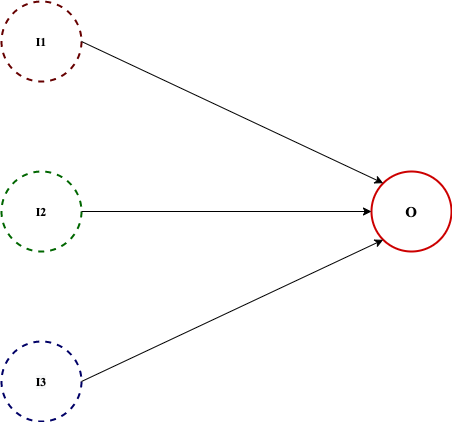
\includegraphics[scale=0.35]{cap2_contextualizacion/images/red_neuronal.png}
    \caption{Red neuronal simple}
    \label{fig:red_neuronal_simple}
\end{figure*}

En la figura \ref{fig:red_neuronal_simple} se muestra una simple red neuronal que consta de 4 neuronas - las neuronas \textbf{\textit{I1}}, \textbf{\textit{I2}} e \textbf{\textit{I3}} corresponden a las neuronas de entrada (\textit{input}) y todas se conectan a la neurona \textbf{\textit{O}}, la neurona de salida (\textit{output}). \\

El funcionamiento de una red neuronal es sencillo - la información se va transfiriendo por las neuronas por medio de \textit{estímulos} que van activando o desactivando las neuronas que componen la red. Para que una neurona \textbf{se active} (también se hace el símil de que la neurona se \textit{dispara}), debe recibir unos estímulos de las neuronas a las que ya están conectadas. La neurona por su lado interpreta este estímulo y, a su vez:

\begin{enumerate}
    \item Se activa (1) y estimula a las siguientes neuronas a las que está conectada
    \item Permanece desactivada (0) y se acaba la interacción 
\end{enumerate}

Un estímulo de una neurona se calcula \textbf{teniendo en cuenta todas las neuronas} activas que están conectadas a la neurona de salida (es decir, la que se desea activar a continuación). Cada conexión entre las neuronas de entrada y salida tiene un peso $\omega$, y la suma ponderada de los pesos es el estímulo total. Para que una neurona se active este estímulo debe ser mayor o igual al umbral de activación $\theta$ de la neurona. \\

Para poder poner un ejemplo se considerará que:

\begin{enumerate}
    \item La neurona O tendrá un umbral de activación de \textbf{4}
    \item La conexión entre la neurona \textit{I1} y la \textit{O} tiene un peso de \textbf{1}
    \item El peso entre la \textit{I2} y \textit{O} es \textbf{2.75}
    \item El peso entre \textit{I3} y \textit{O} es \textbf{0.25}
\end{enumerate} 

En la figura [\ref{fig:red_neuronal_activacion}] se plantean 2 casos distintos: 

\begin{enumerate}
    \item Las neuronas \textit{I1} e \textit{I2} están activas pero la \textit{I3} está inactiva. La suma ponderada de los pesos está por debajo del umbral de activación de la neurona \textit{O}, por lo que no se activará. [\ref{fig:red_neuronal_inactiva}]
    \item Todas las neuronas están activas y la suma ponderada de los pesos es igual al umbral de activación de \textit{O}, por lo que ésta se activará. [\ref{fig:red_neuronal_activa}]
\end{enumerate}

\begin{figure}[h]
    \centering
    \begin{subfigure}{.45\textwidth}
        \centering
        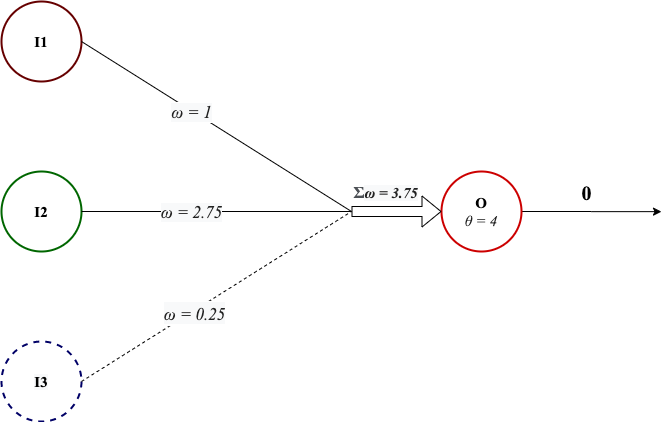
\includegraphics[scale=0.22]{cap2_contextualizacion/images/red_neuronal_inactive.png}
        \caption{I3 inactivo, suma ponderada por debajo del umbral de activación de O}
        \label{fig:red_neuronal_inactiva}
    \end{subfigure}      
    \begin{subfigure}{.45\textwidth}
        \centering
        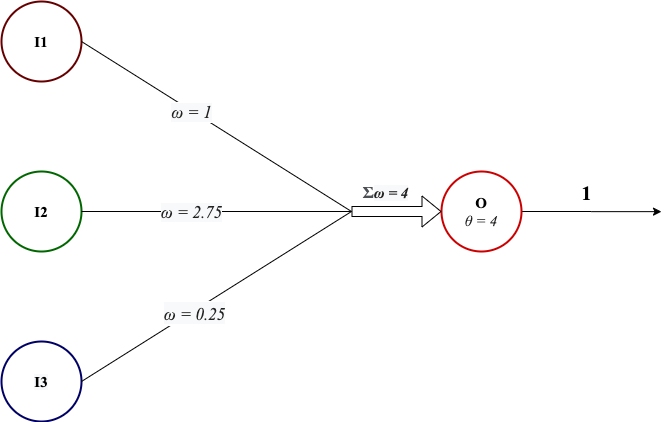
\includegraphics[scale=0.22]{cap2_contextualizacion/images/red_neuronal_active.png}
        \caption{I1, I2, I3 activas, suma ponderada igual al umbral de activación de O}
        \label{fig:red_neuronal_activa}
    \end{subfigure}
    \caption{Activación de la neurona O según las neuronas activas de entrada}
    \label{fig:red_neuronal_activacion}
\end{figure}

\subsection{Entreno de una red neuronal}

Las redes neuronales son ampliamente usadas en las tareas de predicción y de clasificación. Sin embargo, como paso previo a estas tareas es necesario \textit{\textbf{entrenar}} la red. El proceso de entreno sirve para que la red \textit{adquiera experiencia} con los datos, de modo que será capaz de reconocer, clasificar y/o predecir el resultado adecuado con cada dato que se le presenta. \\

En el entreno es necesario disponer de un \textit{conjunto de datos de entrenamiento}. Este \textit{dataset} estará compuesto por distintas muestras - parejas de datos de entrada y de salida con las que la red aprenderá cuáles son las interpretaciones correctas. \\

En cuanto al proceso, el entreno consiste en los siguientes pasos: 
\begin{enumerate}
    \item El agente externo presenta un ejemplo de patrón a la red y observa el comportamiento de \textit{O}
    \item El agente ajusta los pesos de las conexiones en función de estas dos normas:
        \begin{enumerate}
        \item Si el resultado es 0 pero se deseaba una salida de 1, se \textbf{incrementa} el peso de todas las conexiones de las neuronas \textit{activas} que conducen a O (y así se incrementa las probabilidades de que O se active cuando se presenten las mismas condiciones)
        \item Si el resultado es 1 pero se deseaba una salida de 0, se \textbf{decrementa} el peso de todas las conexiones de las neuronas \textit{activas} que conducen a O (y así se incrementa las probabilidades de que O se active cuando se presenten las mismas condiciones)
    \end{enumerate}
\end{enumerate}

Este proceso se realiza varias iteraciones, en cada iteración aplicando este proceso de dos paso a cada muestra del \textit{dataset}. De esta manera se obtiene un \textit{patrón de pesos} de conexiones que permite que la red responda con la salida correcta para todos los ejemplos ofrecidos. \\

\section{Machine Learning. El aprendizaje en inteligencia artificial}


\textbf{\textit{Machine Learning}} o \textit{Aprendizaje automático} hace referencia a la capacidad de una máquina, software u aplicación de aprender mediante la aplicación de algoritmos específicos a cierta entrada de datos de su sistema de manera independiente. \cite{apd2019ml}

\subsubsection{¿Qué es Machine Learning?}
El \textbf{Aprendizaje Automático} consiste en una disciplina de las ciencias informáticas, relacionada con el desarrollo de la Inteligencia Artificial, y que sirve, como ya se ha dicho, para crear sistemas que pueden aprender por sí solos. \\

Es una tecnología que permite hacer automáticas una serie de operaciones con el fin de reducir la necesidad de que intervengan los seres humanos. Como estas acciones se realizan de manera autónoma por el sistema, se dice que el aprendizaje es \textit{automático}.\\

El aprendizaje es la capacidad del sistema para identificar una gran serie de patrones complejos determinados por una extensa cantidad de parámetros. Para que aprenda, el algoritmo interno del sistema se modifica con la constante entrada de datos en la interfaz, y puede, de ese modo, predecir escenarios futuros o tomar acciones de manera automática según ciertas condiciones.

\subsubsection{¿Cómo funciona el Machine Learning?}
En los inicios de la informática el único modo de conseguir que un sistema hiciera algo era escribiendo un algoritmo que definiera el contexto y detalles de cada acción, por lo que el proceo estaba completamente supervisado y controlado por un ser humano. \\

En cambio, los algoritmos que se usan en el desarrollo del \textit{Machine Learning} realizan buena parte de estas acciones por su cuenta. Obtienen sus propios cálculos según los datos que se recopilan en el sistema, y cuantos más datos obtienen, mejores y más precisas serán las acciones resultantes. \\

El éxito de un buen sistema de aprendizaje automático se encuentra en la construcción y adaptación de los árboles de decisiones en base a los datos previamente conocidos por el sistema. Sin embargo, también influye la \textbf{aplicación de fórmulas heurísticas} en los nodos que forman el árbol mediante las que elabora un sistema de inferencias. \\

El sistema de Machine Learning \textbf{necesita contar con un volumen de datos de relevancia para poder suministrar respuestas realmente válidas}. Es decir, cuantos más datos tiene para entrenar y con los que aprender, mejores predicciones, clasificaciones, análisis, etc. será capaz de realizar. Al igual que en la estadística clásica, cuantos más muestras se tenga de la población más se podrá generalizar y crear un sistema que sea capaz de reconocer el mayor número de casos posibles. 

\subsection{Tipos de aprendizaje}

Un sistema de aprendizaje automático utiliza sus experiencias y las evidencias de su entorno como datos para identificar y analizar por sí mismo patrones, comportamientos, relaciones del entorno, etc. De esta manera, adquiere una capacidad de elaborar predicciones de escenarios o iniciar operaciones que son la solución para una tarea específica. \\

A partir de un gran número de ejemplos de un mismo escenario \textbf{se puede elaborar un modelo que deduzca y generalice el comportamiento observado}. \textbf{Una vez construido el modelo se podrán realizar predicciones para casos totalmente nuevos}. \\

En la sección anterior se ha explicado brevemente cómo se prepara y entrena una red que sigue un \textit{aprendizaje supervisado}. El entreno al fin y al cabo es la forma que tiene la red de \textbf{aprender}, de convertirse en \textit{inteligente}. El aprendizaje en inteligencia artificial es uno de los pilares más importantes, y existen tres categorías distintas: el \textbf{aprendizaje supervisado}, el \textbf{aprendizaje no supervisado}, y el \textbf{aprendizaje por refuerzo}. En la figura \ref{fig:ml_tipos_aprendizaje} se muestran todas las aplicaciones de cada uno de los aprendizajes. 
 
\begin{figure*}[h]
    \centering
    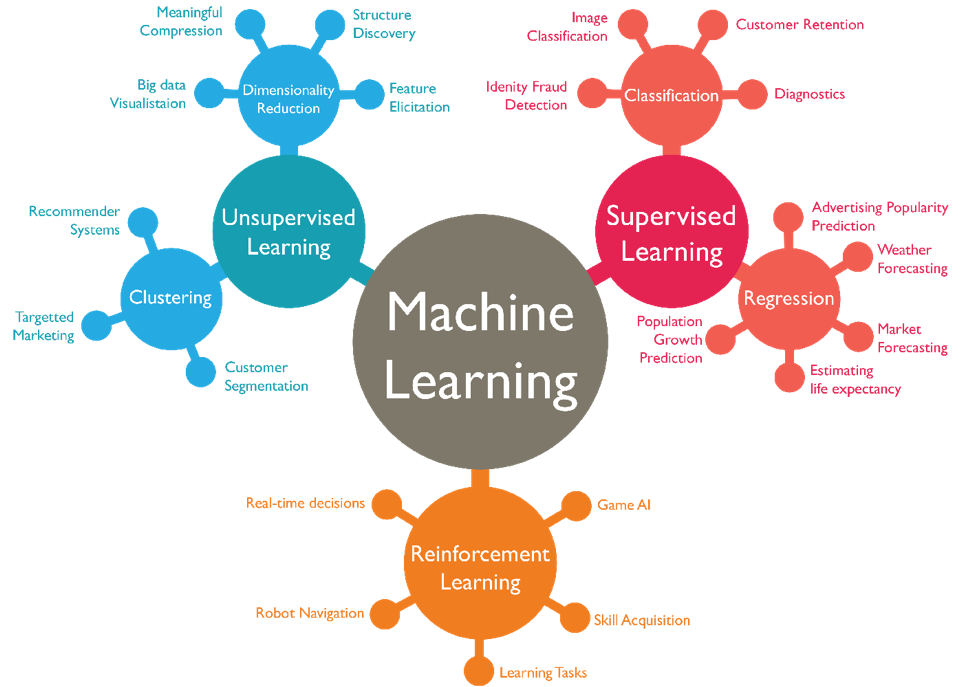
\includegraphics[scale=0.5]{cap2_contextualizacion/images/ml_learning.png}
    \caption{Tipos de aprendizaje en Machine Learning \cite{chugh2008mltypes}}
    \label{fig:ml_tipos_aprendizaje}
\end{figure*}


\subsubsection{Aprendizaje supervisado}

El \textit{aprendizaje supervisado} se basa en la existencia de \textbf{\textit{muestras etiquetadas}} con las que el modelo \textbf{aprende a identificar} los distintos ejemplos que se los proporciona \textbf{por sus etiquetas}: aprende a \textit{clasificarlos}. Para hacer un símil con la naturaleza humana, es como estar enseñándole un objeto a un niño  y diciéndole qué es para que lo pueda reconocer en un futuro. \\

Una vez que se le ha proporcionado la suficiente cantidad de dichos datos, podrán introducirse nuevos datos sin necesidad de etiquetas, en base a patrones distintos que ha venido registrando durante el entrenamiento. Este sistema se conoce como \textbf{\textit{clasificación}}. \\

Otro método de desarrollo del Aprendizaje Automático consiste en predecir un valor continuo, utilizando parámetros distintos que, combinados en la introducción de nuevos datos, permite predecir un resultado determinado. Este método se conoce como \textbf{\textit{regresión}}. \\

Lo que distingue al Aprendizaje Supervisado es que se utilizan distintos ejemplos a partir de los que generalizar para nuevos casos. \\

\subsubsection{Aprendizaje no supervisado}

En cambio, en el \textit{aprendizaje no supervisado} se entrena con datos sin etiquetas - el modelo analiza los datos y se crea él sus propias etiquetas, sus propios grupos, según distintos estrategias de análisis (por distancia, generalmente). \\

Estos sistemas tienen como finalidad la comprensión y abstracción de patrones de información de manera directa, concepto que se conoce como \textbf{\textit{clustering}}.

Este tipo de aprendizaje es más complejo que el anterior, pero es capaz de encontrar relaciones y patrones en los datos que los humanos no serían capaces de reconocer. \\

Un ejemplo de aplicación de este aprendizaje es la clasificación de los compradores en base a sus intereses y a su historial de compras. Este análisis podría mostrar una relación entre la información demográfica de una persona y sus tendencias de compras. \\

\begin{figure*}[h]
    \centering
    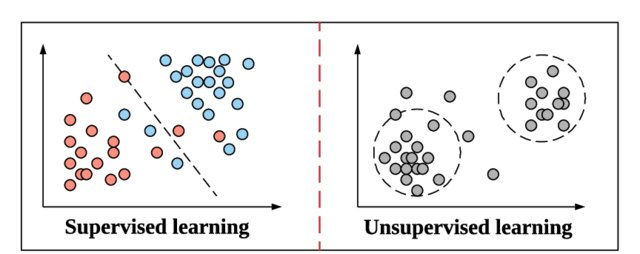
\includegraphics[scale=1]{cap2_contextualizacion/images/diff_sup_unsu.jpg}
    \caption{Aprendizaje supervisado vs. no supervisado}
    \label{fig:diff_sup_unsu}
\end{figure*}

\subsubsection{Aprendizaje por refuerzo}

En la técnica de \textit{aprendizaje por refuerzo} el aprendizaje se realiza por medio de la \textbf{\textbf{prueba y error}}, por lo que los sistemas aprenden completamente a partir de la experiencia - sin intervenciones humanas ni datos con etiquetas. Mediante el uso de funciones de premio que optimizan su comportamiento, el sistema se consigue ser \textbf{\textit{totalmente autónomo}}. \\

A modo de resumen, en la figura \ref{fig:ml_ceralytics} se puede observar un ejemplo de cómo sería entrenar un robot:

\begin{itemize}
    \item En el aprendizaje supervisado se le dice al robot que el objeto es un cubo y éste lo memoriza.
    \item En el aprendizaje no supervisado al robot se le dan dos tipos de piezas y los divide en grupos según su forma.
    \item En el aprendizaje por refuerzo el robot no tiene ninguna información externa pero mediante las percepciones (las formas del hueco y de la figura) y las interacciones (intentar introducir la figura en ambos huecos y ver si entra o no) con su entorno llegará, con el tiempo, a reconocer en qué hueco debe ir la pieza.
\end{itemize}
\begin{figure*}[h]
    \centering
    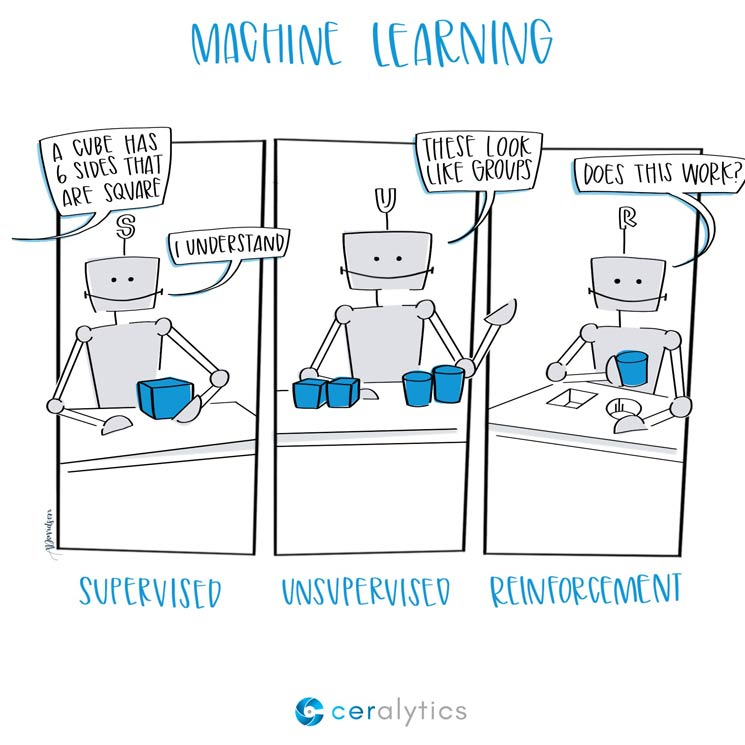
\includegraphics[width=0.45\textwidth]{cap2_contextualizacion/images/machine-learning_ceralytics.jpg}
    \caption{Cómo se diferencian los distintos tipos de aprendizaje en Machine Learning \cite{ceralyticsMLtypes}}
    \label{fig:ml_ceralytics}
\end{figure*}
\subsection{Reinforcement Learning}

El trabajo realizado se basa en el tercer tipo de aprendizaje: \textbf{el aprendizaje por refuerzo}. En este tipo de aprendizaje, la información con la que se entrena al modelo se adquiere mediante las distintas interacciones que el sistema tiene con el entorno del problema dado. \\

Las interacciones vienen definidas, de tal manera que se conoce para cada una de ellas qué efecto tendrá en el entorno, pero no está definido su significado. La manera de discriminar y de enseñarle al sistema que se ha realizado la interacción adecuada para alcanzar su objetivo se hace mediante refuerzos, o como también se les conoce, las \textbf{recompensas}. 

%!TeX root=MemoriaTFG.tex

\chapter{Análisis del proyecto} \label{analisis_proyecto}


Este capítulo recoge toda la información sobre la metodología de desarrollo empleada para el desarrollo del trabajo, los requerimientos  funcionales del proyecto, las restricciones y los objetivos cuantificables que se esperan alcanzar al final del trabajo.

\section{Metodología de desarrollo del proyecto}

Durante la realización de un proyecto es necesario seguir una serie de pautas que permitan la organización, la estructuración y el control del trabajo realizado para procurar seguir una correcta fluidez de desarrollo. Dichas pautas se recogen dentro de los llamados \textbf{\textit{modelos de desarrollo de software}}. Existen distintos tipos de modelos, como por ejemplo el modelo en cascada, el modelo iterativo y el modelo incremental. \\ 

El trabajo realizado para este proyecto ha sido basado en el llamado \textit{modelo de prototipado}, ya que se ha ido implementado, probando y modificando el código y los experimentos a lo largo del desarrollo hasta alcanzar un sistema estable. 

\subsection{El modelo de prototipado}

El \textbf{modelo de prototipado}, también denominado como \textbf{\textit{modelo de desarrollo evolutivo}} o \textbf{\textit{modelo de prototipado incremental}}, se basa en la creación de un (o varios) prototipo del producto final antes de empezar con la implementación del producto. De esta manera es muy sencillo entender cómo será el aspecto y qué características y funcionalidades tendrá el producto final. \\

Tal como aparecen en \cite{modeloPrototipos2}, las características del prototipo son: 

\begin{enumerate}
    \item Es una \textbf{aplicación que funciona}: contiene las funcionalidades desarrolladas a $"$bajo nivel$"$ para que el usuario pueda utilizarlo como si se tratase del producto final y, de esta manera, generar opiniones sobre su funcionamiento.
    \item Se \textbf{crea con rapidez}: debido a que no se tienen que desarrollar las funcionalidades teniendo en cuenta la seguridad, la fiabilidad, la eficacia, u otros aspectos importantes en la implementación, la creación de los prototipos es muy rápida. 
    \item \textbf{Evoluciona} a través de un proceso iterativo:  Con cada prototipo realizado los usuarios lo utilizan y ofrecen una retroalimentación con su experiencia. Cada \textit{feedback} recibido sirve para ajustar las características del prototipo, por lo que cuanto más rápido se reciba dicha respuesta, más rápido se creará el prototipo perfecto con el que se realizará el producto final. 
    \item Tiene un \textbf{coste bajo de desarrollo}: no se deben incorporar servicios costosos ni tener un gran equipo de desarrollo puesto que no se trata del producto final. 
\end{enumerate}

Como bien se menciona en \cite{calameoModeloPrototipado}, \textit{el éxito del uso del prototipo depende de la rapidez y de la frecuencia con la que se reciba el \textbf{feedback} del usuario para hacer cambios y adecuarlos a las necesidades actuales}. Aplicado al proyecto en cuestión, y el usuario final siendo la persona que ha realizado el TFG, 

\begin{itemize}
    \item La \textit{rapidez} es prácticamente inmediata ya que el usuario final y el desarrollador son el mismo.
    \item La \textit{frecuencia} es después de cada experimentación realizada; se valora el prototipo y se aplican las modificaciones necesarias para generar uno nuevo y volver al proceso de experimentación.
\end{itemize}

\subsection{Etapas del modelo de prototipado}

La implementación del software cuando se trata de este tipo de modelo es \textbf{\textit{iterativa}}, ya que se debe diseñar el prototipo, implementarlo y testearlo con usuarios final varias veces hasta tener un prototipo satisfactorio. \\

\begin{figure}[h]
    \centering
    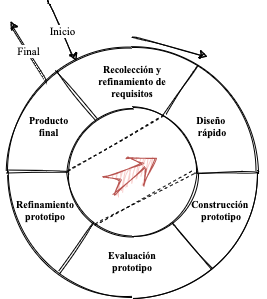
\includegraphics[width=0.3\textwidth]{cap3_analisis_tecnico/images/modelo_prototipado.png}
    \caption{Fases del modelo de prototipado}.
    \label{fig:modelo_prototipado}
\end{figure}

De acuerdo con la definición de \cite{modeloPrototipos1} se ha desarrollado la Fig. ~ \ref{fig:modelo_prototipado} y, cómo se puede apreciar, existen 6 fases en este modelo:

\begin{enumerate}
    \item \textbf{Recolección y refinamiento de requerimientos }: se plantean las características que se desea que tenga el producto final: aspecto, funcionalidad, restricciones, etc. 
    \item \textbf{Diseño rápido}: se diseña el prototipo a partir de las especificaciones ofrecidas.
    \item \textbf{Construcción prototipo}: se implementa el prototipo.
    \item \textbf{Evaluación prototipo}: se evalúa con los usuarios finales.
    \item \textbf{Refinamiento prototipo}: se analiza el \textit{feedback} y si es necesario se hacen cambios en el prototipo. En caso de que esto ocurra, se vuelve a la etapa 2 de diseño.
    \item \textbf{Producto final}: el prototipo ya está listo y se pasa a implementar el producto final. En el caso de este proyecto el producto final es el \textbf{último prototipo} desarrollado que se obtiene al cabo de todo el proceso; es suficiente ya que se trata de una investigación y que, además, dicho prototipo permite conseguir toda la información necesaria para obtener conclusiones válidas del estudio. 
\end{enumerate}



\subsection{Ventajas del modelo de prototipado}
Las ventajas de este modelo son las siguientes \cite{modeloPrototipos1, modeloPrototipos2, ventajasDesventajasPrototipos}: 

\begin{itemize}
    \item \textbf{Útil cuando se conocen los objetivos generales} para el software pero \textbf{no se identifican los requerimientos  detallados} de entrada, procesamiento o salida. Permiten el desarrollo de un sistema a partir de requerimientos  poco claros o cambiantes.
    \item \textbf{No modifica el flujo del ciclo de vida} ya que hasta que se desarrolle un prototipo final no se sale de la etapa de diseño.
    \item \textbf{Aumentan las probabilidades de éxito debido al constante \textit{feedback} que hay sobre el sistema}; esto hace que sea improbable que el producto final no sea el esperado.
    \item \textbf{Reduce el riesgo de construir productos que no satisfagan las necesidades de los usuarios} porque estos están constantemente probándolo y aportando ideas de mejora de usabilidad.
    \item  \textbf{Son más fáciles de abordar con los usuarios finales.} Su uso redunda en una mayor satisfacción del usuario con el producto final, ya que él o ella han participado activamente de su diseño. \textbf{Curva menor de aprendizaje} al comenzar a usar el sistema final. 
    \item \textbf{Permite a todos los involucrados entender bien y mejor el problema antes de la implementación final.}
    \item Se \textbf{reduce el riesgo} o la \textbf{incertidumbre sobre la implementación del software} ya que antes de empezar con el producto final, el prototipo ya estará muy bien estudiado por lo que se conocerán cuáles son las necesidades de implementación.
    \item Como información complementaria a los requerimientos  constituyen un \textbf{gran apoyo a las estimaciones de esfuerzo de todas las áreas}, incluyendo proveedores.
\end{itemize}

\subsection{Desventajas del modelo de prototipado}
Las desventajas de este modelo son las siguientes \cite{modeloPrototipos1, modeloPrototipos2, ventajasDesventajasPrototipos}: 

\begin{itemize}
    \item En la implementación \textbf{el prototipo puede ser modificado y/o ampliado por sus desarrolladores sin consultar} con el cliente, rompiendo así el compromiso de calidad y mantenimiento que tiene con éste.
    \item \textbf{Adoptarlo como el sistema final:} los usuarios y profesionales de sistemas pueden considerar al prototipo como el sistema final cuando aún es incompleto e inadecuado.
    \item \textbf{Los usuarios suelen enfocarse en aspectos “superficiales” del prototipo cuando lo prueban y centrarse menos en su funcionalidad global.} También es posible que se pierda mucho tiempo, innecesariamente, tratando de hacer entender al usuario la finalidad real de los prototipos.
    \item Requiere \textbf{participación activa del usuario} puesto que sus opiniones acerca del prototipo son las que se utilizan para determinar si el prototipo necesita más refinamiento. 
    \end{itemize}

\section{Objetivos}

El objetivo principal de este proyecto es estudiar la capacidad de un agente de aprender a llegar a una casilla en concreto dentro de una matriz después de presentarle con distintas situaciones en las que ha interactuado con el entorno. \\

En cuanto a objetivos más concretos, se quiere:

\begin{enumerate}
    \item Crear un entorno estático y un entorno dinámico para poder presentarle al agente la aleatoriedad de los elementos que percibe y así pueda entrenar bajo condiciones variadas. Por ejemplo, cambio de la meta o del origen, deshabilitación de casillas, etc. 
    
    \item Crear varios modelos para el agente y analizar los datos que genera: media de pasos dados para llegar a la meta, desviación típica de los pasos, error total realizado con los pasos, etc. 
    
    \item Encontrar una conFig. ~ción de ANN
    \begin{enumerate}
        \item Con un mínimo de 10 capas ya que es más probable que el algoritmo converja en una solución. 
        \item Que permita alcanzar una solución con una desviación típica \textit{menor a 3}, porque de lo contrario significaría que el agente no ha llegado a aprender correctamente, es decir, no se ha llegado a una solución.  
    \end{enumerate}
\end{enumerate}


\section{Requerimientos funcionales}

Este proyecto no consta de requerimientos funcionales ya que el sistema no se espera que tenga unos resultados en concreto ni ofrezca un servicio en particular, sino que se trata de una \textbf{experimentación} con la que se llegará a unas conclusiones al cabo de su realización; por lo que, a priori, no es sencillo predecir qué resultados se obtendrán. 
\section{Requerimientos no funcionales}

En cuanto a los requerimientos  funcionales, se tiene: 

\begin{enumerate} \label{requerimientos}
    \item \textbf{RF01}: El proyecto debe hacer uso del \textbf{aprendizaje por refuerzo} para el desarrollo del agente inteligente.
    \item \textbf{RF02}: El proyecto debe implementar el entorno del problema mediante la librería \textit{Gym} de OpenAI \cite{gymDocumentation}.
    \item \textbf{RF03}: El proyecto debe tener el modelo del agente implementado con una \textbf{red neuronal} (\textbf{ANN}).
\end{enumerate}

\section{Herramientas utilizadas para el desarrollo}

En este apartado se detallarán los medios utilizados para la implementación de este proyecto: el lenguaje empleado, las tecnologías, las herramientas y las librerías. 
\subsection{Lenguaje de programación} 

En la actualidad hay un total de 16 lenguajes distintos para el desarrollo de programas de inteligencia artificial \cite{wikiAILanguages}. Para poder elegir un lenguaje es necesario analizar las características y las ventajas de cada uno de ellos y, junto con los requerimientos del proyecto, decidir qué lenguaje es el que mejor se adapta al problema. \\

Debido al elevado número de opciones, se han ido descartando hasta quedar con los más empleados en los últimos años: \textbf{\textit{R}} y \textbf{\textit{Python}}. \\

\textbf{R} es altamente enfocado a la estadística, trato de datos, análisis numéricos y, por supuesto, el Aprendizaje Máquina. \\

\textbf{Python}, por otro lado, se usa en una multitud de ámbitos y consta de una gran comunidad y un gran nombre de librerías. \\

Para la implementación del proyecto se ha elegido el lenguaje \textbf{Python} ya que:

\begin{itemize}
    \item Es \textbf{\textit{fácil de utilizar}} y el código resultante es \textbf{\textit{muy comprensible}}.
    \item \textbf{\textit{Gran número de librerías}} que implementan partes de código necesarios y que, además, supondría una carga añadida si fuese necesario programarlo. En la siguiente sección se concretarán las librerías empleadas. El uso de una librería en concreto, la de Tensorflow, es el motivo principal por el que se ha elegido emplear Python ya que se proporciona una API específica; con R, las bibliotecas son de terceros. 
    \item \textbf{\textit{Comunidad extensa}} y muy implicada, por lo que muchas dudas que puedan surgir a la hora de la implementación es probable que ya esté resuelta si se busca.
\end{itemize}

\subsection{Librerías} 

En el desarrollo de los distintos elementos que componen el proyecto se han utilizado librerías específicas que contienen funciones que facilitan su implementación. A continuación se enumeran las librerías empleadas para cada uno de estos elementos: el \textit{entorno}, el \textit{agente} y los \textit{resultados gráficos}. 

\subsubsection{Librerías para el entorno}

Uno de los requerimientos  de este proyecto era emplear \textit{\textbf{Gym}} \cite{gymDocumentation}, una librería desarrollada por OpenAI que proporciona herramientas para la creación de los entornos empleados en el aprendizaje por refuerzo. \\

Las herramientas de las que dispone \textit{Gym} son empleadas para

\begin{enumerate}
    \item Definir el entorno en el que se encuentra el problema.
    \item Obtener las observaciones y las recompensas obtenidas de una interacción entre agente-entorno \ref{fig:gym_ML}; éstas serán las que determinarán el aprendizaje del agente ya que son indicadores de su comportamiento. Un ejemplo de observación sería: \textit{el agente está a 3 pasos de la meta}. 
\end{enumerate}

Dentro de la librería existen diferentes entornos ya desarrollados y clasificados por el \textit{tipo de problema que se desea resolver}:  \textbf{classic control/toy text}, \textbf{algorithmic}, \textbf{atari}, y  \textbf{2D \& 3D robots} \cite{gymDocumentation}. En el caso de este proyecto, no se ha utilizado ninguna de estas plantillas de entornos, sino que se ha implementado usando como base la clase principal de \texttt{Env} que se encuentra en \textit{Gym}.  \\

Se ha utilizado la última versión \textbf{0.17.1}.

\subsubsection{Librerías para el agente}

Por otro lado, para poder implementar la red neurona, es decir, el agente inteligente, se han utilizado las librerías:

\begin{enumerate}
    \item \textbf{\textit{Tensorflow}} (v. 2.0.0): es una biblioteca de código abierto para \textit{aprendizaje automático}; a través de ésta se pueden desarrollar sistemas capaces de construir y entrenar redes neuronales para detectar y descifrar patrones y correlaciones \cite{tensorflowWikipedia}. Los elementos mediantes los cuales se construyen los sistemas son los llamados \textit{\textbf{tensors}}, estructuras multidimensionales de datos. 
    \item \textbf{\textit{Keras}} (v. 2.3.1): \textit{framework} enfocado al \textit{aprendizaje profundo} (es un tipo de aprendizaje en el que se utilizan redes neuronales de un tamaño considerable, como sería por ejemplo una red de 50 capas con 100 neuronas cada una). Se trata de una API a alto nivel (es decir, es sencilla de emplear y de entender) para las funciones de \textit{Tensorflow}. Los elementos básicos que se tratan en esta biblioteca son las \textbf{capas} (el término en inglés \textit{layers}, son agrupaciones de \textit{tensors}) y los \textbf{modelos}. Los modelos se corresponden, en definitiva, a la red neuronal que se construye, y las operaciones que ofrece dicha librería sirven para realizar el entreno de la red y las posteriores predicciones. 
\end{enumerate}

\subsubsection{Librerías para los resultados gráficos}

Para la representación de los datos y la creación de los gráficos se ha empleado la librería \textbf{\textit{matplotlib}}. Mediante dicha librería es posible 

\begin{itemize}
    \item \textbf{Crear visualizaciones estáticas}; existen muchísimas opciones para producir representaciones \cite{matplotlibGallery}, entre ellas: 
    \begin{itemize}
        \item Líneas, barras y marcadores
        \item Imágenes, contornos y campos
        \item Ejes y Fig. ~s
        \item Elementos estadísticos
        \item Diagramas de tarta y polares
    \end{itemize}
    \item \textbf{Crear visualizaciones dinámicas}, ya que trabaja con distintos \textit{toolkits} de interfaz de usuario (wxpython, tkinter, qt4, gtk, y macosx) \cite{matplotlibUserEvents}; esto posibilitan las interacciones por teclado y ratón, por ejemplo para poder ampliar Fig. ~s. 
\end{itemize}

Se ha utilizado la última versión \textbf{3.1.1}.

\subsubsection{Librerías comunes}

Por último, se ha utilizado las librerías de \textbf{\textit{NumPy}} y \textbf{\textit{Pandas}} para el trato de los datos. 

\begin{itemize}
    \item \textbf{Numpy}: Librería fundamental en la computación científica dentro de Python \cite{numpyDoc}. \\

    Proporciona estructuras del \textbf{tipo multidimensional} (\textit{arrays} y elementos derivados tales como las matrices) y un conjunto de rutinas para operaciones rápidas sobre los arrays, entre las cuales se encuentran las \textbf{matemáticas}, las \textbf{lógicas}, la \textbf{manipulación de las estructuras}, la \textbf{ordenación} y \textbf{selección} de los elementos, la \textbf{entrada/salida} de los elementos, aplicaciones de \textbf{álgebra lineal} y operaciones \textbf{estadísticas} básicas sobre los elementos, y muchas más. \\

    Se ha utilizado la versión \textbf{1.17.4}.
    \item \textbf{Pandas}: Librería que proporciona \textbf{estructuras de datos} (\textit{sencillas} y de \textit{alto rendimiento}) y herramientas para el análisis de datos dentro de Python \cite{pandasDoc}. \\

    Las estructuras de datos son \textbf{rápidas}, \textbf{flexibles} y \textbf{expresivas} y han sido diseñadas con el fin de facilitar el trabajo con datos de tipo \textit{relacional} y \textit{con etiquetas}. Entre las fortalezas de esta librería destacan: 

    \begin{itemize}
    \item \textbf{Facilidad de tratar y adaptar} las estructuras con datos que faltan (NaN), tanto los datos de punto flotante como los que no lo son. 
    \item \textbf{Manipulación sencilla de las dimensiones de los datos} (agregación y eliminación de columnas).
    \item \textbf{Alineamiento de datos automáticos o explícitos}. Los objetos se pueden alinear explícitamente por una serie de etiquetas, o el usuario puede omitir las etiquetas y dejar que las propias estructuras alineen los datos. 
    \item \textbf{Fácil conversión de estructuras de \textit{Python} y \textit{NumPy} a estructuras \textit{pandas}.}
    \item \textbf{Conjunto de operaciones flexibles para aplicar las técnicas de \textit{split-apply-combine}} a los conjuntos de datos; \textit{split} se refiere a la separación de los datos siguiendo un criterio en concreto, \textit{apply} a la aplicación de una función de manera independiente a grupos de datos, y \textit{combine} a la agrupación de los resultados en una única estructura de datos \cite{pandasSplitApplyCombine}.
    \item \textbf{Herramientas de entrada/salida} para el trato de ficheros CSV, Excel, bases de datos, y guardado en formato HDF5. 
\end{itemize}

    Se ha utilizado la última versión \textbf{1.1.2}.

\end{itemize}

\subsection{Software y otros elementos} 

En cuanto a los programas utilizados, se ha empleado el programa \textbf{PyCharm} de JetBrains ya que es en IDE intuitivo, fácil de usar, con integración de GIT, visualización de gráficos, visualización de bases de datos, sencillo proceso para debuggear el código, etc. \\

También se ha empleado la herramienta \textbf{Git} para el control de versiones del proyecto. \\


En este capítulo se ha descrito \textit{la metodología} abordada para el desarrollo del proyecto, se han enumerado los distintos \textit{requerimientos } y \textit{objetivos} planteados y se han explicado las diferentes \textit{herramientas} empleadas en la implementación, desde el lenguaje elegido hasta las distintas librerías empleadas. 

%!TeX root=MemoriaTFG.tex

\chapter{Diseño e implementación del proyecto} \label{diseño_implementacion}

En este capítulo se recogen las características de diseño del proyecto, así como también su posterior implementación. A continuación se detallarán cómo son el programa principal, el agente y el entorno del problema, cómo se relacionan, y finalmente, cómo están implementados. 

\section{Diseño del proyecto}

Para poder realizar la implementación del proyecto, es necesario diseñar los elementos principales que lo conforman: el programa principal que controla la ejecución, la definición de los elementos empleados en el programa y las distintas funcionalidades que se desea que tengan.  

\subsection{Diseño del programa}

El programa principal es el elemento de control de la ejecución. Se ha diseñado de tal forma que el usuario tiene control casi al completo de todas las características de la ejecución de un experimento a partir de sus especificaciones concretas. Además, el usuario también podrá elegir de la lista de experimentos previamente realizados y podrá ver las gráficas con los resultados obtenidos. \\

Las especificaciones del usuario sobre el experimento son:
\begin{enumerate}
    \item Las \textbf{iteraciones} y los \textbf{episodios} totales del experimento.
    \item Las \textbf{dimensiones} del entorno.
    \item El \textbf{tipo de ejecución} de desea realizar, si bien un nuevo experimento o la visualización de  resultados de experimentos anteriores. 
    \item El \textbf{tipo de modelo} que se debe emplear. Los distintos tipos se explicarán en el apartado \ref{tiposModelos}.
    \item El \textbf{tipo de experimento} que se quiere llevar a cabo. Los experimentos que se pueden realizar se explicarán en el apartado \ref{tiposExperimentos}.
\end{enumerate}

El experimento puede contener varias iteraciones, con cada iteración un total de episodios concreto. Los episodios hacen referencia a la veces que el agente busca su camino hacia el objetivo. Con cada episodio, el entorno se reinicia a su estado inicial y se comienza de nuevo. Los episodios pueden llegar a una solución o no. \\

El objetivo de tener distintas iteraciones, además de entrenar la red, es para\textit{ modificar las condiciones del entorno} y \textit{observar la adaptación del agente}. Las condiciones que se modifican son las \textbf{posiciones del agente} y del \textbf{objetivo}. 

\subsubsection{Tipos de modelos} \label{tiposModelos}

Los modelos hacen referencia al modelo interno del agente que compone la red neuronal. El modelo puede ser
\begin{itemize}
    \item Un \textbf{modelo nuevo}, es decir, una red neuronal inicializada con sus pesos aleatoriamente y sin entreno previo. 
    \item Un \textbf{modelo existente}; dicho modelo ya habrá sido sometido a uno o varios experimentos, por lo que tendrá los pesos ya ajustados con unos valores determinados. 
\end{itemize}

Una vez realizado un experimento se puede guardar el modelo resultante y los resultados de dicho experimento. 


\begin{figure}[ht!]
    \centering
    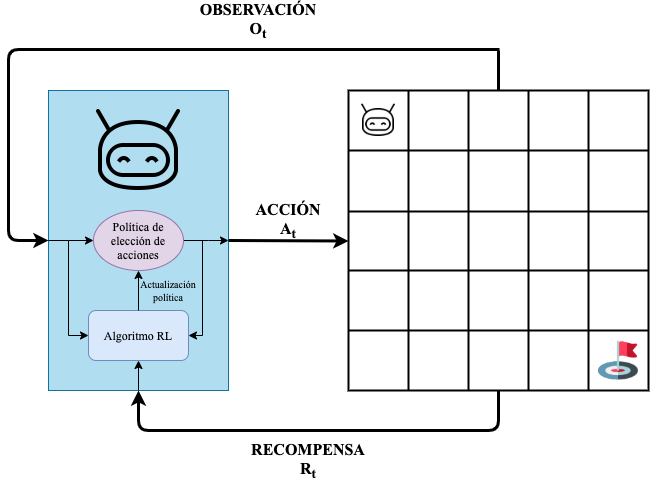
\includegraphics[scale=0.5]{cap4_diseño_implementacion/images/diagrama_RL.png}
    \caption{Ecosistema del proyecto compuesto por el entorno y el agente.}
    \label{fig:red_neuronal_simple}
\end{figure}

El problema propuesto, como bien se ha mencionado anteriormente en el capítulo \ref{introduccion}, tiene un ecosistema formado por: 
\begin{enumerate}
    \item Un \textbf{entorno} que contiene toda la información del problema: la \textbf{estructura} del espacio en el que se desarrollan las acciones, las \textbf{dimensiones} del espacio, las \textbf{acciones} que se pueden realizar, las \textbf{percepciones} observables que describen cómo va cambiando el entorno con cada acción realizada y, por último, las \textbf{recompensas} que se reciben con cada acción dependiendo del estado en el que se encuentra el entorno. 
    \item Un \textbf{agente inteligente} que debe interaccionar con el entorno con el fin de cumplir un objetivo definido. Las interacciones que puede tener con el entorno van definidas por una serie de acciones concretas. 
\end{enumerate}

En la Fig.~\ref{fig:red_neuronal_simple} se puede observar dicho ecosistema con los elementos y las interacciones posibles entre ellos. \\

A continuación se detallará el diseño de ambos elementos a alto nivel. 

\subsection{Diseño del entorno}

Para el diseño del entorno se deben tener en cuenta su \textit{estructura}, las \textit{acciones que se pueden realizar}, las \textit{percepciones} y las \textit{recompensas} que se ofrecen al agente. 

\subsubsection{Modelización del entorno} 

El entorno del problema tiene una \textbf{estructura matricial} y se muestra en la Fig.~\ref{fig:estructura_entorno}. Las dimensiones del entorno son \textbf{\textit{dinámicas}} - no hay un tamaño fijo definido sino que se permite minimizar o ampliar las dimensiones. 

\begin{figure}
    \centering
    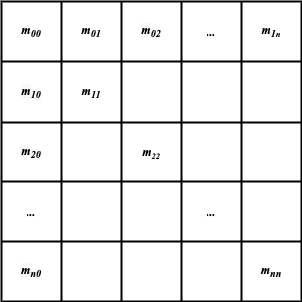
\includegraphics[scale=0.4]{cap4_diseño_implementacion/images/entorno.png}
    \caption{Estructura del entorno.}
    \label{fig:estructura_entorno}
\end{figure}

\subsubsection{Acciones permitidas}

Sea $n$ la dimensión de la matriz, $x$ el índice de las filas e $y$ el índice de las columnas de la matriz del entorno. El rango de los valores se encuentra entre de $x$ e $y$ entre $0 - (n - 1)$. Las acciones permitidas para el desplazamiento dentro de este entorno son: 
\begin{enumerate}
    \item \textbf{\textit{Arriba}}: desplazamiento de una casilla $m_{xy}$ a una casilla $m_{xy-1}$.
    \item \textbf{\textit{Abajo}}: desplazamiento de una casilla $m_{xy}$ a una casilla $m_{xy+1}$.
    \item \textbf{\textit{Derecha}}: desplazamiento de una casilla $m_{xy}$ a una casilla $m_{x+1y}$.
    \item \textbf{\textit{Izquierda}}: desplazamiento de una casilla $m{xy}$ a una casilla $m_{x-1y}$. 
\end{enumerate}
Dichas acciones se representan en la Figura \ref{fig:acciones_entorno}. \\
\begin{figure}
    \centering
    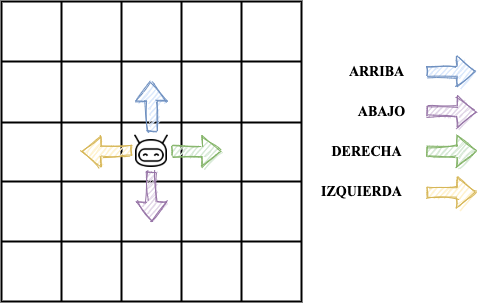
\includegraphics[scale=0.5]{cap4_diseño_implementacion/images/acciones.png}
    \caption{Acciones del entorno.}
    \label{fig:acciones_entorno}
\end{figure}

En la nomenclatura de la librería \textit{Gym}, el número total de acciones que se realizar hacer se denomina $action\_space$, es decir, espacio de acciones.

\subsubsection{Percepciones del entorno} En el entorno se conoce en cada \textbf{\textit{estado}} cuál es la \textbf{posición exacta del agente}; los estados, por lo tanto, codifican una posición de la matriz. Los estados no contemplan si se ha llegado al objetivo, sino que se comprueba con cada movimiento realizado si el nuevo estado en el que se encuentra el entorno se corresponde con la \textbf{posición del objetivo} que se debe alcanzar. \\

\begin{figure}[!h]
    \centering
    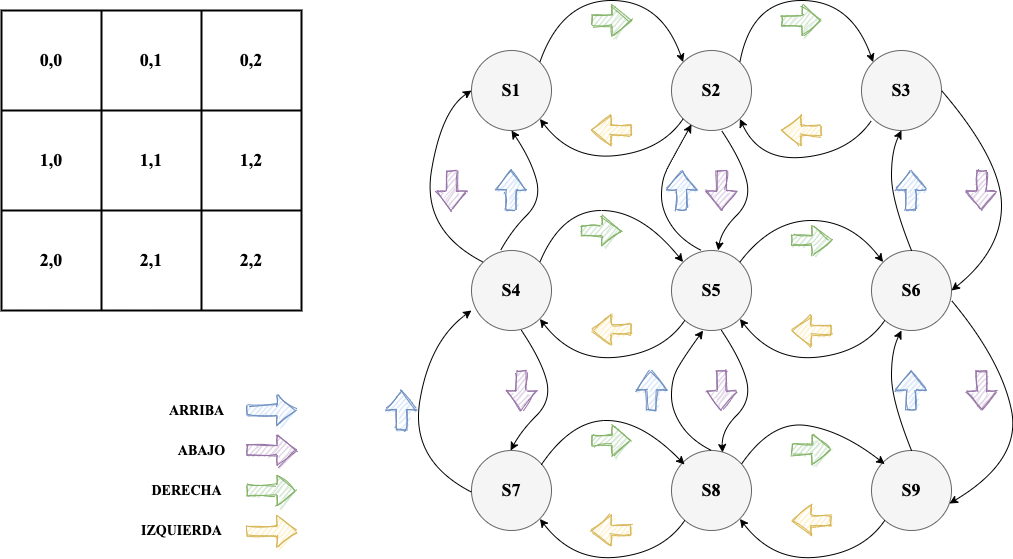
\includegraphics[scale=0.4]{cap4_diseño_implementacion/images/estados_3x3.png}
    \caption{Ejemplo de diagrama de estados de un entorno con una dimensión de 3x3.}
    \label{fig:estados_3x3}
\end{figure}

Los \textbf{estados totales} que puede tener el entorno viene determinado por sus dimensiones, y se calcula como $n^2$. Como se puede observar en la Fig.~\ref{fig:estados_3x3}, un entorno con unas dimensiones de $3x3$ tendría un \textbf{total de 9 estados diferentes}. \\

En la nomenclatura de la librería \textit{Gym}, el número total de estados en el que se puede encontrar el entorno se denomina $observation\_space$, es decir, espacio de observaciones (percepciones).

\subsubsection{Recompensas} 

Una recompensa es aquella percepción del entrono que muestra si la acción realizada anteriormente ha supuesto un avance hacia el objetivo del agente. Las recompensas son aquellas que el agente valorará para determinar si su comportamiento es eficiente y si le permite acercarse cada vez más al objetivo. \\

Existen 2 tipos de recompensas: 

\begin{enumerate}
    \item El agente deberá recibir \textbf{una recompensa positiva} siempre que haga \textbf{una acción lógica dentro del entorno} que le perimta estar más cerca del objetivo propuesto. 
    \item El agente deberá recibir \textbf{una recompensa negativa} cuando realice \textbf{una acción que le suponga estar más lejos de su objetivo}, o bien cuando realiza una acción que implique salir del rango permitido del entorno. 
\end{enumerate}


\begin{figure}
    \centering
    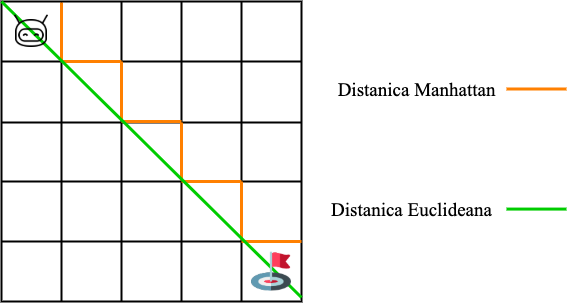
\includegraphics[scale=0.4]{cap4_diseño_implementacion/images/recompensa_distancia.png}
    \caption{Distancia de Manhattan y Euclideana en una matriz de dimensiones 5x5.}
    \label{fig:recompensa_distancia}
\end{figure}

\begin{figure}
    \centering
    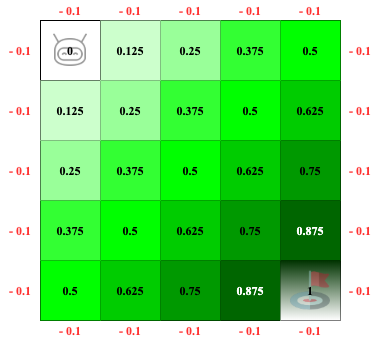
\includegraphics[scale=0.55]{cap4_diseño_implementacion/images/rewards_5x5.png}
    \caption{Recompensas del entorno de 5x5 según la distancia al objetivo. Se considera que el objetivo está en la posición (4, 4).}
    \label{fig:rewards_5x5}
\end{figure}

En el caso de las recompensas positivas, éstas se calculan teniendo en cuenta la \textbf{distancia de Manhattan} entre la posición del agente y la posición del objetivo. Se ha elegido este tipo de distancia debido a la naturaleza de la estructura del entorno (matricial) y a las acciones que se pueden realizar. \\

La recompensa se ha normalizado para tener valores entre 0 y 1, y se calcula de la siguiente forma: 

$$ d_{normalizada} = 1 - \frac{d_{Manhattan}} {d_{maxima}}$$


Cuanto más cerca esté el agente del objetivo, la recompensa recibida será mayor. Se puede observar la evolución de la recompensa en la Fig.~\ref{fig:rewards_5x5}.


\subsection{Diseño del agente} \label{diseñoAgente}

Uno de los requisitos del proyecto (véase Req.~\ref{requerimientos}) era \textbf{la necesidad de utilizar una red neuronal} para el agente. \\

En la figura \ref{fig:NN4_25_25_4} se muestra la red implementada para este problema. La dimensión y las capas de la red neuronal utilizada para la experimentación surgió tras la realización de diversas pruebas. Se optó por mantener este modelo constante a lo largo de las diferentes pruebas con el objetivo de simplificar la interpretación de los resultados.\\

El algoritmo de aprendizaje empleado para la red neuronal es el \textbf{DQN}, explicado anteriormente en el apartado \ref{dqn-learning}. 

\begin{figure}
    \centering
    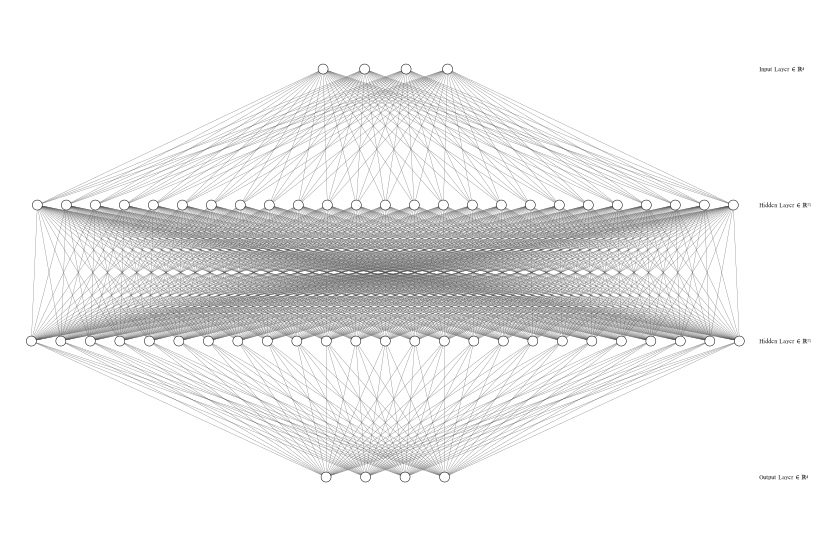
\includegraphics[scale=0.45]{cap4_diseño_implementacion/images/NN4_25_25_4.png}
    \caption{Red neuronal de 4 capas con 4, 25, 25, 4 neuronas, respectivamente.}
    \label{fig:NN4_25_25_4}
\end{figure}

\section{Implementación del proyecto}

Los detalles más significantes de la implementación se detallan a continuación. La Fig.~\ref{fig:diagrama_RL_funciones} sintetiza aquellas funciones implementadas dentro del modelo del entorno y del agente. De derecha a izquierda, tenemos:

\begin{enumerate}
    \item La implementación del entorno, en la que se muestra la estructura que lo compone y un ejemplo de transición entre estados mediante la realización de una acción por parte del agente. El entorno, una vez realizada la acción, devuelve una serie de percepciones al agente. 
    \item La implementación del agente, en la que se muestran los componentes que permiten el aprendizaje y las distintas interacciones que tiene con el entorno. Los componentes de aprendizaje son la política de acciones $\pi$, la función \texttt{replay}, la memoria de repetición $\mathbbb{D}$.
\end{enumerate}

\begin{figure}
    \centering
    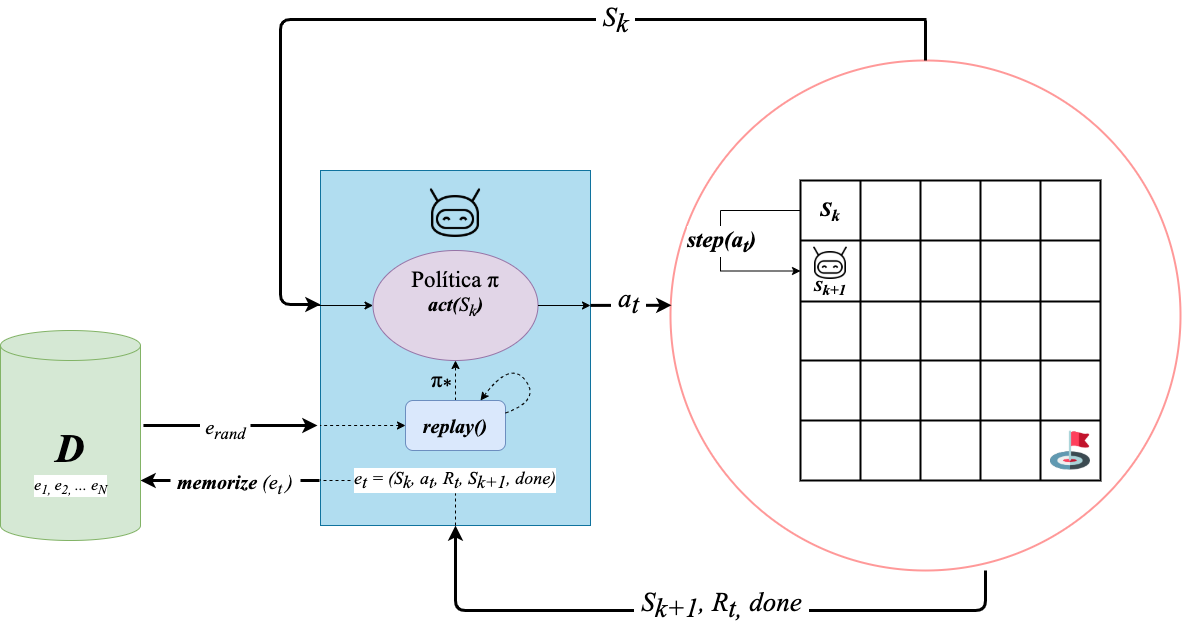
\includegraphics[scale=0.39]{cap4_diseño_implementacion/images/diagrama_RL_funciones.png}
    \caption{Implementación del ecosistema del problema.}
    \label{fig:diagrama_RL_funciones}
\end{figure}
A continuación se explicará el programa principal que se encarga de controlar la ejecución del proyecto. 

%TODO ISAAC-WAIT-SECCION
\subsection{Implementación del programa}

La implementación del programa principal se encarga de encajar todas las piezas (el agente y el entorno y sus características) y de realizar la ejecución siguiendo las especificaciones del usuario. Recordemos que el usuario puede especificar: 
\begin{enumerate}
    \item El total de iteraciones y de episodios que tendrá el experimento. 
    \item Las dimensiones del entorno.
    \item El tipo de ejecución de desea realizar.
    \item El tipo de modelo que se debe emplear. 
    \item El tipo de experimento que se quiere llevar a cabo. 
\end{enumerate}

Los métodos más importantes del programa son: 

\begin{enumerate}
    \item \texttt{run\_experiment}: Controla las iteraciones del experimento y recoge todos los resultados de cada una. Además, si es necesario, modifica las posiciones del agente o del objetivo. 
    \item \texttt{compute\_iteration}: Como el propio nombre indica, realiza una iteración con todos sus episodios. \\
    
    En cada episodio $ep$ se resetea el entorno a su estado inicial $S_0$ y se lanza el agente para que encuentre la combinación de movimientos que lleve al objetivo. Si se llega al objetivo, se actualiza el target con los Q-values actuales (tal como está explicado en el apartado \ref{dqn-learning-replay}). Cuando la memoria de repetición $D$ haya sobrepasado una cierta cantidad de experiencias $MAX\_MEMORY$ se lanzará la función de \texttt{replay} para aprender de la experiencia. \\

\subsubsection{Función \texttt{compute\_iteration}}

La función que controla la ejecución y las distinta interacciones entre el entorno y el agente es la función \texttt{compute\_iteration}, y se muestra en el Alg. ~\ref{compute_iteration}. \\

Este método se ejecuta tantas veces como iteraciones haya definido el usuario. Para cada episodio que hay en una iteración (línea ~\ref{lst:line:computeIterationLine1}), se resetea el estado del entorno a su estado inicial $S_0$ (línea ~\ref{lst:line:computeIterationLine2}). A continuación se realiza la búsqueda de la secuencia de acciones que lleven al objetivo. El número máximo de acciones que puede realizar el agente viene definido por la variable $steps$. Las acciones se calculan teniendo en cuenta el estado actual del entorno (línea~\ref{lst:line:computeIterationLine4}); una vez elegida la acción el agente se mueve dentro del entorno (línea ~\ref{lst:line:computeIterationLine5}) y guarda la experiencia resultante en la memoria de repetición (línea ~\ref{lst:line:computeIterationLine6}). El estado del entorno se actualiza y, en caso de que se haya alcanzado el objetivo, se guarda el modelo actual como el óptimo (línea ~\ref{lst:line:computeIterationLine9}) y se termina la ejecución del episodio. Si el tamaño de la memoria de repetición ha superado la cantidad $MAX\_MEMORY$, se realiza el aprendizaje empleando la función \texttt{replay} (línea ~\ref{lst:line:computeIterationLine12}), explicado en el Alg. ~\ref{replayAlgorithm}. \\
\begin{algorithm}[H]
\SetAlgoLined
\SetKwInOut{Input}{input}
\SetKwInOut{Output}{output}
\SetKw{KwIn}{in}
\SetKw{KwBreak}{break}
\SetKw{KwNot}{not}
\SetKwData{Episodes}{$episodes$}
\SetKwData{Episode}{$ep$}
\SetKwData{Actions}{$actions$}
\SetKwData{Step}{$t$}
\SetKwData{Steps}{$steps$}
\SetKwData{BatchSize}{$batch\_size$}
\SetKwData{Done}{$done$}
\SetKwData{Action}{$a_t$}
\SetKwData{MaxMem}{$MAX\_MEMORY$}
\SetKwData{State}{$S_k$}
\SetKwData{InitialState}{$S_0$}
\SetKwData{NextState}{$S_{k+1}$}
\SetKwData{Env}{$env$}
\SetKwData{Agent}{$agent$}
\SetKwData{Reward}{$R_t$}
\SetKwData{Memory}{$D$}
\SetKwData{IterationResults}{$iteration\_results$}
\SetKwData{EpsSolved}{$episodes\_solved$}
\SetKwData{StepsTaken}{$steps\_taken$}
\SetKwData{EpisodeRewards}{$episode\_rewards$}
\SetKwData{EpisodeReward}{$episode\_reward$}
\SetKwFunction{Append}{append}
\SetKwFunction{ComputeIteration}{$compute\_iteration$}
\SetKwFunction{Act}{act}
\SetKwFunction{StepAction}{step}
\SetKwFunction{Memorize}{memorize}
\SetKwFunction{Len}{len}
\SetKwFunction{UpdateTargetModel}{$update\_target\_model$}
\SetKwFunction{Replay}{replay}
\Input{$episodes$}
\BlankLine
\For{\Episode \KwIn \Episodes}{\label{lst:line:computeIterationLine1}
    \State $\leftarrow$ \InitialState\;\label{lst:line:computeIterationLine2}
    \For{\Step \KwIn \Steps}{
        \Action $\leftarrow$ \Agent.\Act{\State}\;\label{lst:line:computeIterationLine4}
        \NextState, \Reward, \Done $\leftarrow$ \Env.\StepAction{\Action}\;\label{lst:line:computeIterationLine5}
        \Agent.\Memorize{\State, \Action, \Reward, \NextState, \Done}\;\label{lst:line:computeIterationLine6}
        \State $\leftarrow$ \NextState\;
        \uIf{\Done}{
            \Agent.\UpdateTargetModel{}\;\label{lst:line:computeIterationLine9}
            \KwBreak\;
        }
        \uIf{\Len{\Memory} > \MaxMem}{
            \Agent.\Replay{\BatchSize}\;\label{lst:line:computeIterationLine12}
        }  
    }
}
 \caption{Función \texttt{compute\_iteration}} \label{compute_iteration}
\end{algorithm}
\end{enumerate}

\subsection{Implementación del entorno}

La implementación del entorno se ha realizado mediante la clase básica de la librería \textit{Gym}: \texttt{Env} \cite{gymCore}. Las operaciones que define son:

\begin{enumerate}
    \item \texttt{\textbf{step}}: Aplica una acción $a$ al entorno. Dicha acción provoca un cambio de estado en el entorno, y éste devuelve como resultados de esta función
    \begin{enumerate}
        \item \texttt{\textit{observation}}: El nuevo estado de entorno.
        \item \texttt{\textit{reward}}: La recompensa obtenida a raíz de la realización de la acción $a$.
        \item \texttt{\textit{done}}: Determina si el episodio ha acabado, es decir, si se ha llegado al objetivo. 
        \item \texttt{\textit{info}}: Sirve para imprimir información auxiliar que puede ser útil para \textit{debuggear}. 
    \end{enumerate}
    \item \texttt{\textbf{reset}}: Resetea el entorno a su estado inicial y retorna dicho estado. 
    \item \texttt{\textbf{render}}: Visualiza el entorno. Existen varios modos de visualización: $human$, $rgb\_array$ y $ansi$.
    \item \texttt{\textbf{close}}: Finaliza el programa y limpiar
    la memoria. En caso de que no se implemente, el propio entorno $"$se cierra$"$ cuando el programa se cierra. 
    \item \texttt{\textbf{seed}}: Fija la \textit{semilla} de generación pseudoaleatoria de número que controlan las interacciones con el agente. 
\end{enumerate}

De estos 5 métodos \textbf{se han sobrescrito 2, \textit{\texttt{step}} y \textit{\texttt{reset}}}. \\

\subsubsection{Función \texttt{step}}

La función \texttt{step}, como ya se ha mencionado, corresponde a la realización de la acción ($a_t$) dentro del entorno. Para poder aplicar la acción $a_t$ se debe primero eliminar el agente de la posición $agent\_pos$ en la que estaba antes de realizar la acción (línea ~\ref{lst:line:stepLine1} del Alg. ~\ref{stepAlgorithm}). Una vez hecho esto, se calcula su nueva posición $next\_agent\_pos$ (línea ~\ref{lst:line:stepLine2}) teniendo en cuenta la acción elegida $a_t$ y se actualiza el entorno con la nueva posición (línea ~\ref{lst:line:stepLine3}). Por último, se calcula la recompensa total obtenida $R_t$ (línea ~\ref{lst:line:stepLine5}) tras realizar este movimiento, y se comprueba si el agente ya ha llegado a la posición del objetivo (línea ~\ref{lst:line:stepLine6}). La función GetReward se describe en el Alg. ~\ref{GetReward}. 

\begin{algorithm}[H]
\SetAlgoLined
\SetKwInOut{Input}{input}
\SetKwInOut{Output}{output}
\SetKwData{NextAgentPos}{$next\_agent\_pos$}
\SetKwData{Penalty}{$use\_penalty$}
\SetKwData{Reward}{$R_t$}
\SetKwData{Done}{$done$}
\SetKwData{AgentPos}{$agent\_pos$}
\SetKwData{Action}{$a_t$}
\SetKwData{GoalPosition}{$goal\_position$}
\SetKwData{State}{$S_k$}
\SetKwData{NextState}{$S_{k+1}$}
\SetKwFunction{GetReward}{GetReward}
\SetKwFunction{GetNextPosition}{GetNextPosition}
\Input{$a_t$}
\Output{$S_{k+1}, R_t, done$}
\BlankLine
\State[\AgentPos] $\leftarrow$ $0$\;  \label{lst:line:stepLine1} 
\NextAgentPos, \Penalty $\leftarrow$ \GetNextPosition{\Action,\AgentPos}\;\label{lst:line:stepLine2} 
\State[\NextAgentPos] $\leftarrow$ $1$\; \label{lst:line:stepLine3} 
\NextState $\leftarrow$ \State\;
\Reward $\leftarrow$ \GetReward{\NextAgentPos, \Penalty}\;\label{lst:line:stepLine5} 
\Done $\leftarrow$ \NextAgentPos $\equiv$ \GoalPosition\; \label{lst:line:stepLine6}
return \NextState, \Reward, \Done\;
 \caption{Función \textit{\texttt{step}}} \label{stepAlgorithm}
\end{algorithm} 

\subsubsection{Función \texttt{GetReward}}

La función \texttt{GetReward}, mostrada en el Alg.~\ref{GetReward}, sirve para calcular la recompensa obtenida después de un movimiento realizado. Para calcular la recompensa $R_t$ se necesita la posición actual de agente $agent\_pos$; además, se tiene una variable $use\_penalty$ que indica si el movimiento realizado previamente ha causado que el agente salga del rango del entorno: en caso afirmativo, en lugar de recompensa el agente recibe una penalización con valor de -0.1 (línea ~\ref{lst:line:getRewardLine2}). Si de lo contrario el movimiento era válido, se calcula la distancia Manhattan (línea ~\ref{lst:line:getRewardLine4}) de la posición actual del agente hasta la posición del objetivo. La distancia normalizada (línea ~\ref{lst:line:getRewardLine5}) se corresponde a la recompensa que se devuelve (línea ~\ref{lst:line:getRewardLine7}). \\

\begin{algorithm}[H]
\SetAlgoLined
\SetKwInOut{Input}{input}
\SetKwInOut{Output}{output}
\SetKwData{Reward}{$R_t$}
\SetKwData{Penalty}{$use\_penalty$}
\SetKwData{AgentPos}{$agent\_pos$}
\SetKwData{Distance}{$d_{manhattan}$}
\SetKwData{MaxDistance}{$d_{maxima}$}
\SetKwData{GoalPosition}{$goal\_position$}
\SetKwFunction{Cityblock}{cityblock}
\Input{$agent\_pos$, $use\_penalty$}
\Output{$R_t$}
\BlankLine
\eIf{\Penalty}{
   \Reward $\leftarrow$ $-0.1$ \; \label{lst:line:getRewardLine2}
   }{
\Distance $\leftarrow$ \Cityblock{\AgentPos, \GoalPosition} \;\label{lst:line:getRewardLine4}
\Reward $\leftarrow$ 1 - (\Distance / \MaxDistance) \;\label{lst:line:getRewardLine5}
}
return \Reward \;\label{lst:line:getRewardLine7}
 \caption{Función \textit{\texttt{GetReward}}} \label{GetReward}
\end{algorithm}

\subsection{Implementación del agente}

El agente se ha implementado utilizando el modelo \texttt{Sequential} de la librería \texttt{Keras}. Tal como se explica en la documentación oficial de Keras \cite{kerasSequential}, este modelo \textit{se utiliza para una simple agrupación de capas donde cada capa tiene exactamente un tensor de entrada y un tensor de salida}. \\

La arquitectura de la red neuronal empleada se compone por 4 capas de 4, 25, 25, 4 neuronas respectivamente, y se muestra en la Fig. ~\ref{fig:NN4_25_25_4}. Las distintas capas tienen como función de activación: 

\begin{itemize}
    \item \textbf{linear}: Las primeras 3 capas de la red. La salida de las neuronas se calculan teniendo en cuenta la suma de los valores de las entradas multiplicadas por los pesos de cada una. 
    \item \textbf{softmax}: La última capa, ya que es interesante ver los resultados de la red como un porcentaje para que la interpretación sea más intuitiva. Tal como se explica en \cite{activationFunctionTypes}, esta función trata con múltiples clases y es capaz de normalizar la salida de la red para cada clase para que tengan valores entre 0 y 1. Estos valores, además, representan las probabilidades que tiene cada acción de ser elegida.
\end{itemize}

\begin{figure}
    \centering
    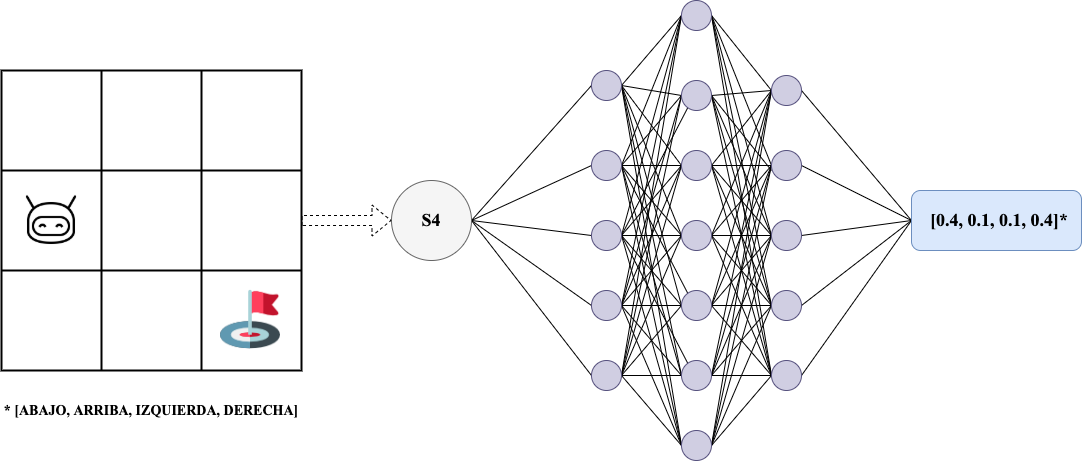
\includegraphics[scale=0.4]{cap4_diseño_implementacion/images/nn_input_output.png}
    \caption{Entrada y salida del agente.}
    \label{fig:nn_input_output}
\end{figure}

En este caso, la entrada del modelo es el \textbf{estado del entorno}, y la salida es una \textbf{lista de predicciones} que se corresponde con las \textbf{probabilidades de cada acción} de realizarse en esas condiciones concretas. \\

Un ejemplo de ello se muestra en la Fig.~\ref{fig:nn_input_output}, donde un agente se encuentra en la posición (1, 0) de la matriz. Dicha posición se corresponde con el estado $S_4$ y a partir de la evaluación de la red neuronal interna del agente se le ha asociado a este estado una probabilidad por cada acción que se puede realizar, en concreto: 0.4 si se mueve hacia abajo, 0.1 si se mueve hacia arriba, 0.1 si se mueve a la izquierda y 0.4 si se mueve a la derecha. \\
   
A continuación se explicarán las funcionalidades del agente implementadas. 

\subsubsection{Función \texttt{act}}

Función que determina \textbf{qué acción $a_t$ es la mejor para tomar a continuación dado un estado $S_k$} en concreto del entorno. Para ello, la red neuronal debe predecir para cada acción la probabilidad $\mathbb{P}_{A}$ de ser elegida; en base a dicha predicción, se escoge la acción con mayor probabilidad de ocurrir y se retorna. \\

\subsubsection{Función \texttt{memorize}}

Función que sirve para \textbf{guardar} en la \textit{memoria de repetición} del agente $D$ \textbf{la experiencia obtenida} $e_t$ compuesta por el estado $S_k$, acción $a_t$, siguiente estado $S_{k+1}$ y si ha llegado al objetivo. Es el proceso de aprendizaje, y mediante este método es como se \textit{construye la experiencia}. 

\subsubsection{Función \texttt{replay}}

Esta función es un tipo de técnica denominada \textbf{\textit{repetición de experiencia}} que se utiliza durante el periodo de entreno de la red. Tal como se explica en \cite{stack2017expreplay, deeplizardReplay}, para cada instante de tiempo $t$ de entreno se guarda una tupla que contiene la experiencia obtenida $e_t = (S_k, a_t, S_{k + 1}, R_t)$. Todas las tuplas de la experiencia del agente se guardan en la \textit{memoria de repetición} $D$, y será de éste conjunto de datos de dónde se tomarán muestras aleatorias para entrenar a la red. \\

En el Alg. ~\ref{replayAlgorithm} se muestra la implementación de la función \texttt{replay}. Inicialmente se comienza seleccionando una cantidad de muestras aleatorias de la memoria de repetición (línea ~\ref{lst:line:replayLine2}) que servirán como muestras de entreno para el agente. Si la red sólo aprendiese de las muestras consecutivas de experiencia que suceden de manera secuencial en el entorno, las muestras estarían altamente correlacionadas y llevaría a un aprendizaje ineficiente. El hecho de seleccionar muestras aleatorias rompe esta correlación. \\

Para cada muestra en concreto se obtiene la recompensa $R_t$ (línea ~\ref{lst:line:replayLine3}) y, en caso de que dicha experiencia no sea una en la que el agente haya alcanzado su objetivo, se recalcula la recompensa (línea ~\ref{lst:line:replayLine5}) aplicándole el descuento $\gamma$ para que refleje que no se ha conseguido alcanzar el objetivo. A continuación, se obtiene la lista de predicciones $target$ para el estado $S_k$ (línea ~\ref{lst:line:replayLine6}) y se le asigna la recompensa calculada $R_t$ al elemento de la lista correspondiente a la acción $a_t$ (línea ~\ref{lst:line:replayLine7}). Finalmente, se entrena la red dados los estados y las listas de predicciones obtenidas previamente (línea ~\ref{lst:line:replayLine11}) y se devuelve el error total obtenido.  \\
\begin{algorithm}[H]
\SetAlgoLined
\SetKwInOut{Input}{input}
\SetKwInOut{Output}{output}
\SetKwData{States}{$states$}
\SetKwData{Targets}{$targets$}
\SetKwData{Reward}{$R_t$}
\SetKwData{History}{$history$}
\SetKwData{ValueReward}{$value\_reward$}
\SetKwData{Memory}{$memory$}
\SetKwData{Random}{$random$}
\SetKwData{Loss}{$loss$}
\SetKwData{Minibatch}{$minibatch$}
\SetKwData{Batchsize}{$batch\_size$}
\SetKwData{Gamma}{$\gamma$}
\SetKwData{Target}{$target$}
\SetKwData{Model}{$model$}
\SetKw{KwIn}{in}
\SetKwData{Done}{$done$}
\SetKwData{Action}{$a_t$}
\SetKwData{State}{$S_k$}
\SetKwData{NextState}{$S_{k+1}$}
\SetKwFunction{Append}{append}
\SetKwFunction{Predict}{predict}
\SetKwFunction{Fit}{fit}
\SetKwFunction{Sample}{sample}
\Input{$batch\_size$}
\Output{$loss$}
\BlankLine
\Minibatch $\leftarrow$ \Random.\Sample{\Memory, \Batchsize}\;\label{lst:line:replayLine2}
\For{\State, \Action, \Reward, \NextState, \Done \KwIn \Minibatch}{\label{lst:line:replayLine2}
    \ValueReward $\leftarrow$ \Reward\;\label{lst:line:replayLine3}
    \uIf {$not$ \Done}{
        \ValueReward $\leftarrow$ (\ValueReward + \Gamma * max(\Model.\Predict{\NextState}))\;\label{lst:line:replayLine5}
    }
    \Target $\leftarrow$ \Model.\Predict{\State}\;\label{lst:line:replayLine6}
    \Target[\Action] = \ValueReward\;\label{lst:line:replayLine7}
    \States.\Append{\State}\;
    \Targets.\Append{\Target}\;
}
\History $\leftarrow$ \Model.\Fit{\States, \Targets}\;\label{lst:line:replayLine11}
\Loss $\leftarrow$ \History[$'loss'$]\;
return \Loss\;
 \caption{Función replay} \label{replayAlgorithm}
\end{algorithm}

\subsubsection{Función \texttt{predict}}

Mediante éste método se invoca al \texttt{predict} correspondiente a la red neuronal (implementado por la clase \texttt{Sequential} de Keras) y se obtienen las predicciones para las acciones posibles. Es necesario conocer el estado actual $S_k$ del entorno para poder realizar la predicción. \\



En este capítulo se ha visto en detalle el diseño y la implementación del proyecto. Se ha visto la estructura del programa principal, así como también el flujo de la interacción entre el entorno y el agente. Para el entorno del problema se han explicado las 2 funciones fundamentales que le permite interactuar con el agente: las funciones \texttt{step} y \texttt{GetReward}. Para el agente se han explicado las funciones que sirven para realizar el aprendizaje, en concreto las funciones \texttt{memorize}, \texttt{replay} y \texttt{predict}, y también la función \texttt{act} que le permite al agente moverse por el entorno. \\

El flujo del programa y de las interacciones entre los elementos es el siguiente: \\
\renewcommand{\labelenumii}{\arabic{enumi}.\arabic{enumii}.}
\renewcommand{\labelenumiii}{\arabic{enumi}.\arabic{enumii}.\arabic{enumiii}.}
\renewcommand{\labelenumiv}{\arabic{enumi}.\arabic{enumii}.\arabic{enumiii}.\arabic{enumiv}.}
\begin{enumerate}
    \item Para \textbf{cada iteración}:
    \begin{enumerate}
        \item Para \textbf{cada episodio} de la iteración: 
        \begin{enumerate}
            \item \textbf{Resetear} el entorno a su estado inicial.
            \item Mientras el número total de acciones realizadas \textbf{no supere} el máximo permitido:
            \begin{enumerate}
                \item \textbf{Encontrar la acción} con más probabilidades de ejecutarse en el estado actual. 
                \item \textbf{Realizar el movimiento} en el entorno. Esto implica: 
                \begin{itemize}
                    \item Eliminar al agente de la posición actual del entorno. 
                    \item \textbf{Calcular la nueva posición} dentro del entorno dado el movimiento realizado.
                    \item \textbf{Actualizar entorno} con la nueva posición del agente. 
                    \item Calcular la \textbf{recompensa} total obtenida. La recompensa se calcula empleando la \textit{distancia de Manhattan} y, además, está normalizada entre los valores 0 y 1. Las recompensas también pueden ser negativas cuando se ha realizado un movimiento no válido, y en este caso tendrá el valor de -0.1.
                    \item Comprobar si \textbf{la nueva posición} del agente es \textbf{la misma que la posición del objetivo}. En caso afirmativo, es que se ha alcanzado el objetivo. 
                \end{itemize}
                \item \textbf{Guardar la experiencia} realizada compuesta por el estado actual, la acción realizada, el siguiente estado tras realizar la acción y la recompensa obtenida a raíz del movimiento en memoria. 
                \item Si se ha alcanzado el objetivo, \textbf{guardar la red} interna del agente como la red óptima y saltar al paso 1.1.1.
                \item Por lo contrario, se comprueba si la memoria ya tiene suficientes experiencias acumuladas y en caso afirmativo \textbf{se entrena la red} empleado muestras de experiencias de la memoria. 
            \end{enumerate}
        \end{enumerate}
    \end{enumerate}
\end{enumerate}
El código completo del proyecto se puede encontrar en este repositorio \cite{git}.\\

%!TeX root=MemoriaTFG.tex

\chapter{Fase de experimentación}

Una vez implementado todo el sistema es necesario realizar una serie de pruebas y experimentos para determinar su capacidad real y comprobar que se cumplen los objetivos planteados. En este capítulo se explica el ámbito de la experimentación, que engloba las condiciones de experimentación, el equipo empleado y los tipos de experimentos realizados, la visualización e interpretación de los resultados obtenidos de los experimentos realizados y, por último, el análisis comparativo de los distintos experimentos.

\section{Ámbito de la experimentación}

El objetivo principal de los experimentos es comprobar si el agente llega a \textbf{converger en una solución}, es decir, llega un momento en el que las recompensas obtenidas se estabilizan debido a que el agente es capaz de alcanzar el objetivo en todos los episodios. 

\subsection{Condiciones de experimentación}

Como bien se ha mencionado en el capítulo anterior, el usuario tiene un papel importante a la hora de la ejecución del programa ya que debe especificar parámetros de la ejecución. Sin embargo, también existen elementos que no se le permite controlar. \\


Dichos elementos son la \textit{posición inicial del agente} y la \textit{posición del objetivo}. Se ha planteado de esta manera para:
\begin{enumerate}
    \item Evitar fallos provocados por el usuario al introducir posiciones no válidas. 
    \item Introducir un elemento de aleatoriedad en los diferentes experimentos, ya que en cada experimento siempre habrá una distancia nueva entre el agente y el objetivo. 
\end{enumerate}

\subsection{Equipo empleado}

El hardware empleado para la realización de los experimentos es un ordenador MacBook Pro con un procesador Quad-Core Intel Core i7 y con una memoria de 16GB. Las especificaciones se muestran en la Fig.~\ref{fig:computer_specs}
\begin{figure}
    \centering
    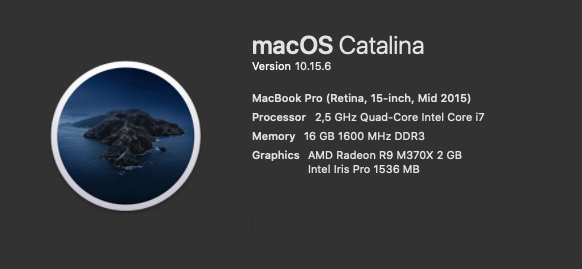
\includegraphics[scale=0.5]{cap5_experimentacion/images/computer_specs.png}
    \caption{Especificaciones del ordenador empleado en la experimentación.}
    \label{fig:computer_specs}
\end{figure}

\subsection{Métricas empleadas y elementos analizados}

El usuario puede guardar resultados obtenidos de los experimentos en estructuras llamadas \textbf{\textit{dataframe}}. \\

Un dataframe es un tipo de estructura que se caracteriza por guardar los datos y organizarlos por columnas y por filas. Cada fila de dicha estructura se corresponde con una iteración del experimento. Los resultados contienen los siguientes campos: 
\begin{enumerate}
    \item \texttt{experimentType}: El tipo de experimento realizado. 
    \item \texttt{modelUsed}: El modelo del agente empleado.
    \item \texttt{episodes}: El total de episodios por iteración.
    \item \texttt{iterations}: El total de iteraciones realizadas. 
    \item \texttt{episode\_results}: Lista de objetos que contiene los resultados de interés de los episodios de cada iteración, en concreto:
    \begin{itemize}
        \item \texttt{episodes}: Número total de episodios por iteración, que se emplea aquí para calcular el error obtenido.
        \item \texttt{steps\_to\_completion}: Lista que contiene el total de pasos realizados en cada episodio para buscar el objetivo. El total de pasos que se pueden realizar pueden estar entre el número óptimo de acciones, que se corresponde a la distancia Manhattan entre el agente y el objetivo, y el número máximo de pasos permitidos para alcanzar el objetivo. Si el número de pasos alcanza el máximo, generalmente significa que no se ha encontrado una solución. 
        \item \texttt{total\_solved}: Número total de episodios en los que se ha encontrado una solución.
        \item \texttt{episode\_reward}: Lista de recompensas para cada episodio.
        \item \texttt{error}: Porcentaje de episodios que han llegado a una solución.
        \item \texttt{distance\_to\_goal}: Distancia entre el agente y el objetivo. 
        \item \texttt{action\_combinations}: Lista que contiene la secuencia de acciones realizadas por episodio para alcanzar el objetivo. Dado que las secuencias se repiten, solamente se guardan aquellas secuencias que han aparecido más de 5 veces en la ejecución. 
    \end{itemize}
    \item \texttt{dimension}: Las dimensiones del entorno. 
    \item \texttt{start\_pos}: La posición inicial del agente.
    \item \texttt{goal\_pos}: La posición del objetivo. 
\end{enumerate}

Las gráficas realizadas con los resultados obtenidos muestra la evolución del total de acciones, de las recompensas recibidas y de la variación de las acciones a lo largo de los episodios realizados. Además, también se muestran las secuencias de acciones más frecuentes que ha aprendido el agente para alcanzar el objetivo, y el número total de veces que dichas secuencias se han aplicado. 

\subsection{Arquitectura de la red neuronal del agente}

A lo largo de la experimentación se ha mantenido estable la arquitectura de la red neuronal del agente. Tal como se ha explicado en el apartado de diseño del agente \ref{diseñoAgente}, la red neuronal consta de 4 capas de 4, 25, 25 y 4 neuronas respectivamente. La red se muestra en la Fig.~\ref{fig:NN4_25_25_4}. \\

No se ha modificado la red en cada experimento porque se ha considerado que si se modifica, la comparación de los resultados no sería válida debido a que no puede determinar qué resultados son mejores si los experimentos no se han llevado a cabo bajo las mismas circunstancias. 

\section{Tipos de experimentos} \label{tiposExperimentos}

Para este trabajo se han implementado 4 tipos de experimentos que puede invocar el usuario:

\begin{enumerate}
    \item \textbf{Estudio de convergencia:} Entorno estático.  Se trata de un experimento estático que \textit{mantiene la misma distancia entre el agente y el objetivo} a lo largo de su ejecución. El objetivo de este experimento es observar si llega un punto en el que el resultado converge en una solución. 
    \item \textbf{Alternando el inicio del agente:} Entorno dinámico. Se realiza el experimento \textit{modificando la posición inicial del agente} con cada iteración de la ejecución. El objetivo de este experimento es observar la adaptación del agente frente al cambio de distancia entre su posición inicial y la del objetivo, y si incluso con un entorno estático consigue encontrar la solución.
    \item \textbf{Alternando la posición del objetivo:} Entorno dinámico. Se realiza el experimento \textit{modificando la posición del objetivo} con cada iteración de la ejecución. El objetivo de este experimento es el mismo que el anterior.
    \item \textbf{Repetir experimento} ya realizando modificando sus condiciones. Entorno dinámico. Este tipo de experimento sólo se puede efectuar con los experimentos de alternación de las posiciones del agente y del objetivo. Dichos experimentos necesariamente deben realizar varias iteraciones ya que se trata de modificar las distancias y ver el comportamiento de la red. Cada iteración, por lo tanto, tiene una distancia concreta. El objetivo de este experimento es ir alternando las distancias de cada iteración y observar si se obtienen resultados distintos al experimento original. 
\end{enumerate}

 
\section{Experimentos realizados}

En todos los episodios, en caso de que no se especifique, se ha empleado un \textit{learning rate} de 0.01, un \textit{exploration rate} de 0.2 y un máximo de pasos que se pueden realizar para alcanzar el objetivo de 60. Se han elegido estos valores tras la realización de varias pruebas iniciales. \\

En la Fig.~\ref{fig:initial} se pueden observar los resultados de un experimento de 1 iteración de 100 episodios y empleando los valores especificados anteriormente. La distancia al objetivo es de 4. Las acciones realizadas (Fig.~\ref{fig:initial_acciones}) se estabilizan en el valor óptimo 4 y no varía mucho su distribución (Fig.~\ref{fig:initial_boxplot}); además, las recompensas con máximas a lo largo de la ejecución (Fig.~\ref{fig:initial_recompensa}) y de los 100 episodios se han resuelto 97 (Fig.~\ref{fig:initial_porcentajeResuelto}). Los resultados obtenidos son muy buenos, por lo que se utilizarán dichos valores en todos los experimentos. \\

\begin{figure}
    \centering
    \begin{subfigure}{.6\textwidth}
        \centering
        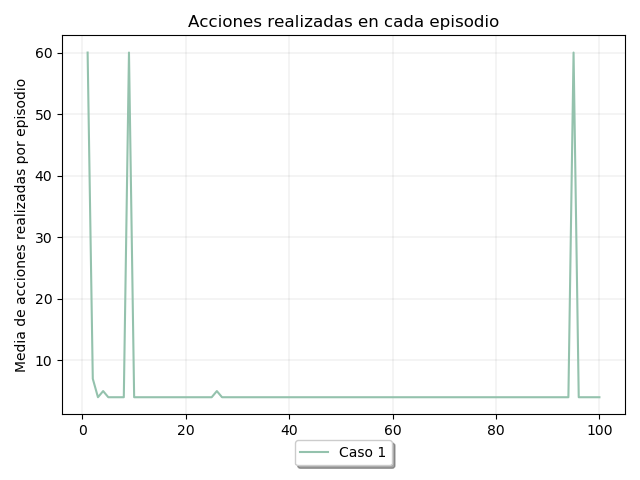
\includegraphics[scale=0.35]{cap5_experimentacion/images/initial_acciones.png}
        \caption{Aplicada 313 veces.}
        \label{fig:initial_acciones}
    \end{subfigure}%      
    \begin{subfigure}{.6\textwidth}
        \centering
        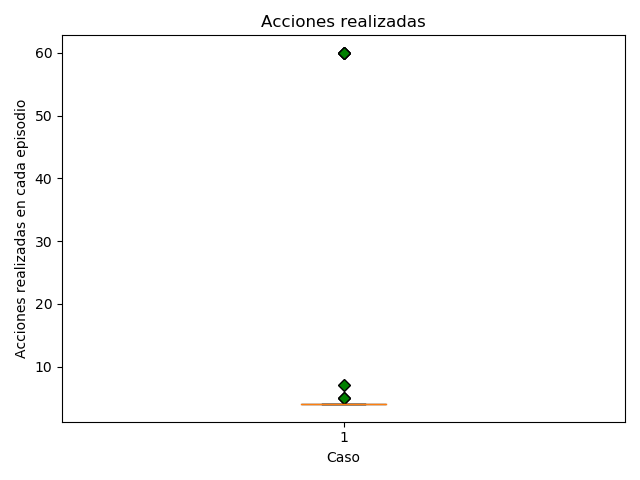
\includegraphics[scale=0.35]{cap5_experimentacion/images/initial_boxplot.png}
        \caption{Aplicada 86 veces.}
        \label{fig:initial_boxplot}
    \end{subfigure}
    \begin{subfigure}{.6\textwidth}
        \centering
        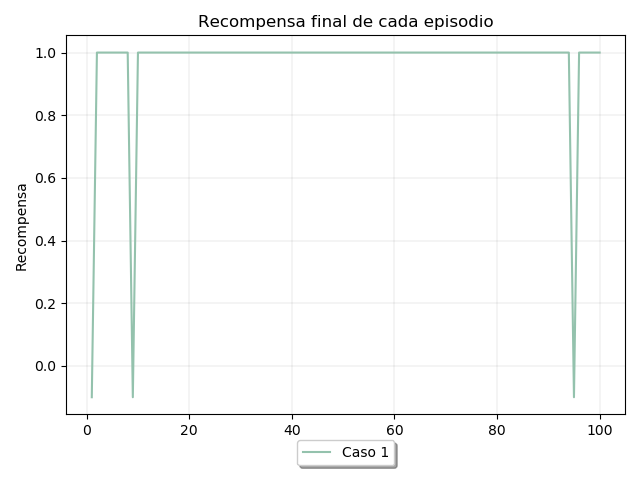
\includegraphics[scale=0.35]{cap5_experimentacion/images/initial_recompensa.png}
        \caption{Aplicada 29 veces.}
        \label{fig:initial_recompensa}
    \end{subfigure}%
    \begin{subfigure}{.6\textwidth}
        \centering
        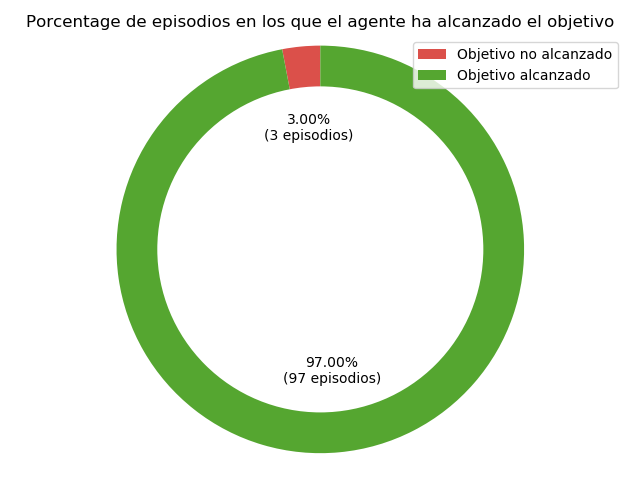
\includegraphics[scale=0.35]{cap5_experimentacion/images/initial_porcentajeResuelto.png}
        \caption{Aplicada 29 veces.}
        \label{fig:initial_porcentajeResuelto}
    \end{subfigure}
    \caption{Experimento de prueba de una iteración de 100 episodios, con \textit{learning rate} de 0.01, \textit{exploration rate} 0.2 y 60 pasos máximos permitidos.}
    \label{fig:initial}
\end{figure}

A continuación se explican los 5 experimentos realizados para determinar la capacidad de la red interna del agente de encontrar una solución para el problema dado. Los distintos experimentos que se han realizado son: 

\begin{enumerate}
    \item \texttt{EPS1}: Estudio de convergencia en un entorno 5x5.
    \item \texttt{EPS2}: Estudio de convergencia con \textit{learning rate} variable.
    \item \texttt{EPS3}: Estudio de convergencia con \textit{exploration rate} variable.
    \item \texttt{CHG\_ORG}: Alternando el inicio del agente en un entorno 5x5.
    \item \texttt{CHG\_GOAL}: Alternando la posición del objetivo en un entorno 5x5.
\end{enumerate}

En todos los experimentos realizados se considera que el \textbf{valor óptimo de acciones} que se pueden realizar para alcanzar el objetivo es equivalente a la distancia Manhattan que hay entre la posición inicial del agente y la posición del objetivo.  

\subsection{EPS1: Estudio de convergencia en un entorno 5x5} \label{EPS1}

Este experimento se ha realizado con 1 iteración de 500 episodios. La posición inicial del agente se ha definido en (0, 0) y la posición del objetivo en (4, 4). La distancia entre el agente y su objetivo es de 8 y se corresponde, además, a la distancia máxima que existe dentro del entorno actual. En la Fig.~\ref{fig:dim5_EPS1} se puede visualizar el entorno del problema con su configuración. \\

\begin{figure}
    \centering
    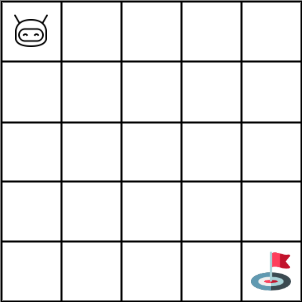
\includegraphics[scale=0.4]{cap5_experimentacion/images/dim5.png}
    \caption{Configuración del entorno para el experimento \texttt{EPS1}.}
    \label{fig:dim5_EPS1}
\end{figure}

El número óptimo de acciones que se pueden hacer para alcanzar el objetivo es 8. 

\subsubsection{Análisis de las acciones realizadas} 

Se puede observar en la Fig.~\ref{fig:dim5_acciones} que a partir de los 80 episodios aproximadamente el número de acciones se estabiliza, alcanzando además el número óptimo de pasos que se deben realizar. Aunque a lo largo de los episodios el número de acciones realizadas alcanza varias veces el valor máximo, no significa que el agente no esté aprendiendo bien. De hecho, es una muestra de que sigue aprendiendo y explorando nuevas secuencias de acciones para realizar.\\

\begin{figure}
    \centering
    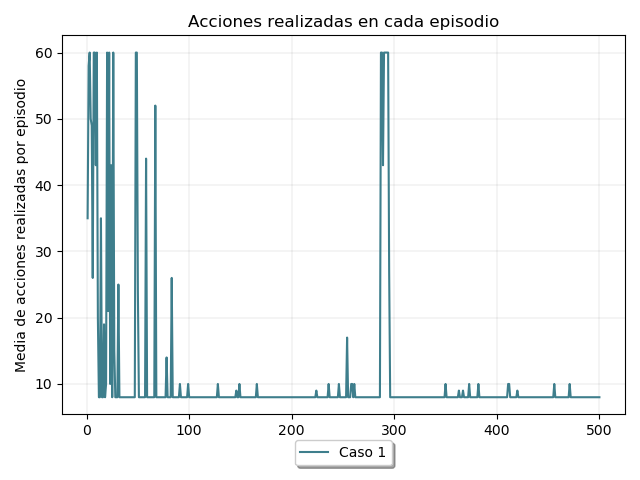
\includegraphics[scale=0.4]{cap5_experimentacion/images/dim5_acciones.png}
    \caption{Acciones realizadas por episodio en el experimento \texttt{EPS1}.}
    \label{fig:dim5_acciones}
\end{figure}

En la Fig.~\ref{fig:dim5_boxplot} se muestra la distribución de las acciones totales realizadas en el experimento. La media de las acciones se corresponde con el valor óptimo, en este caso 8. También se pueden observar otro tipo de elementos en este gráfico: los valores atípicos. Un valor se considera atípico siempre sea una observación que es numéricamente distante del resto de los datos. \\
 
\begin{figure}
    \centering
    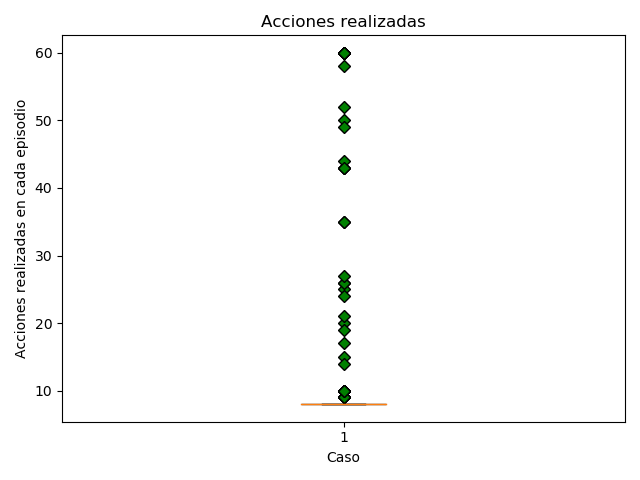
\includegraphics[scale=0.4]{cap5_experimentacion/images/dim5_boxplot.png}
    \caption{Boxplot del experimento \texttt{EPS1}.}
    \label{fig:dim5_boxplot}
\end{figure}

Otro análisis realizado es el estudio de las secuencias de acciones que el modelo ha aprendido para alcanzar el objetivo. Cabe destacar que las secuencias mostradas son las más \textit{frecuentes}. Se considera que una secuencia es frecuente si aparece como solución en más de 5 episodios. Por lo tanto, la suma de las veces que se han aplicado las secuencias frecuentes \textbf{no} es necesariamente equivalente al total de episodios resueltos del experimento. \\

Como bien se observa en la 
Fig.~\ref{fig:dim5_actions}, se han encontrado 4 secuencias diferentes de 8 acciones que llevan al objetivo. La secuencia más frecuente ha sido la de la Fig.~\ref{fig:dim5_actions_313}, con un total de 313 veces que ha sido aplicada. El total de episodios resueltos empleando estas secuencias es de 433.
 
\begin{figure}
    \centering
    \begin{subfigure}{.5\textwidth}
        \centering
        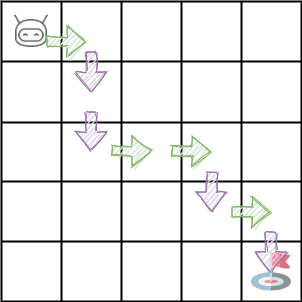
\includegraphics[scale=0.4]{cap5_experimentacion/images/dim5_actions_313.png}
        \caption{Aplicada 313 veces.}
        \label{fig:dim5_actions_313}
    \end{subfigure}%       
    \begin{subfigure}{.5\textwidth}
        \centering
        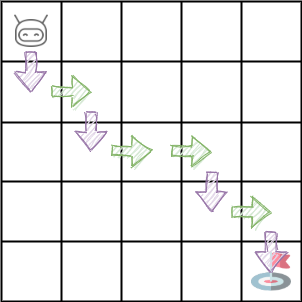
\includegraphics[scale=0.4]{cap5_experimentacion/images/dim5_actions_86.png}
        \caption{Aplicada 86 veces.}
        \label{fig:dim5_actions_86}
    \end{subfigure}
    \begin{subfigure}{.5\textwidth}
        \centering
        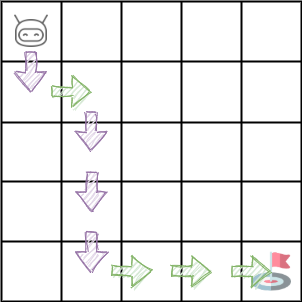
\includegraphics[scale=0.4]{cap5_experimentacion/images/dim5_actions_29.png}
        \caption{Aplicada 29 veces.}
        \label{fig:dim5_actions_29}
    \end{subfigure}%
    \begin{subfigure}{.5\textwidth}
        \centering
        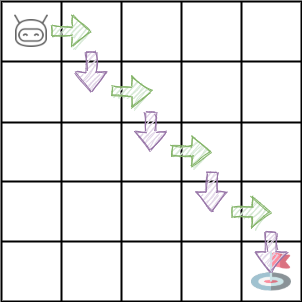
\includegraphics[scale=0.4]{cap5_experimentacion/images/dim5_actions_5.png}
        \caption{Aplicada 5 veces.}
        \label{fig:dim5_actions_5}
    \end{subfigure}
    \caption{Secuencias de acciones realizadas en el experimento \texttt{EPS1} para llegar al objetivo.}
    \label{fig:dim5_actions}
\end{figure}

\subsubsection{Análisis de las recompensas obtenidas y total de episodios resueltos} 

En cuanto a la recompensa obtenida en este experimento, se observa en la Fig.~\ref{fig:dim5_recompensa} que al inicio de la ejecución el agente obtenía valores cercanos al cero, lo que significa que recibía penalizaciones; a partir del mismo episodio en el que el agente comienza a estabilizar las acciones tomada, también se estabiliza la recompensa en su valor máximo y se mantiene en ésta. Recordemos que la recompensa máxima que tiene como valor 1 significa que el agente ha alcanzado su objetivo.\\
 
\begin{figure}
    \centering
    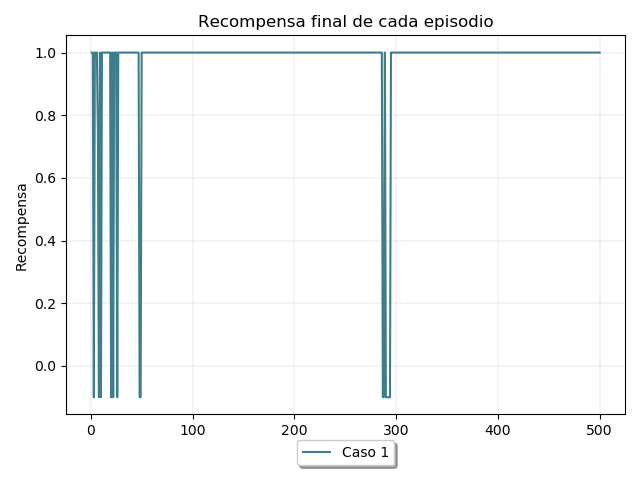
\includegraphics[scale=0.4]{cap5_experimentacion/images/dim5_recompensa.png}
    \caption{Recompensas finales de cada episodio del experimento \texttt{EPS1}.}
    \label{fig:dim5_recompensa}
\end{figure}

En este experimento de 500 episodios, el agente ha sido capaz de alcanzar el objetivo en 484 episodios. En la Fig.~\ref{fig:dim5_porcentajeResuelto} se muestran los porcentajes de episodios resueltos y no resueltos del experimento. Tal como se ha mencionado anteriormente, el total de episodios resueltos no es igual al total de episodios que se han solucionado aplicando las secuencias de la Fig.~\ref{fig:dim5_actions}. En concreto, hay 16  episodios que se han resuelto mediante unas secuencias de acciones poco frecuentes. \\

\begin{figure}
    \centering
    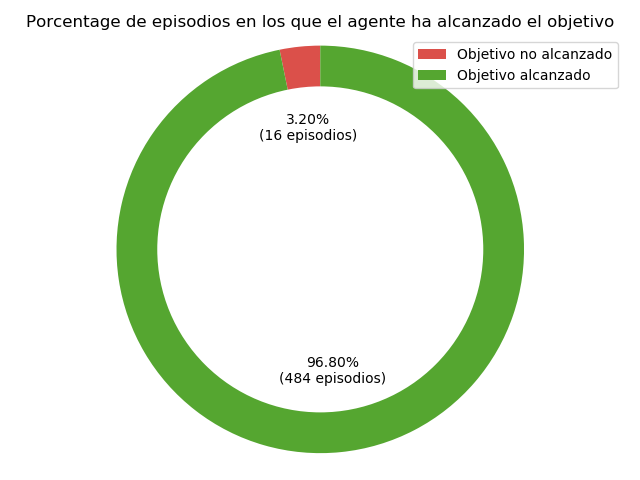
\includegraphics[scale=0.4]{cap5_experimentacion/images/dim5_porcentajeResuelto.png}
    \caption{Porcentaje de episodios en los que el agente alcanza el objetivo en el experimento \texttt{EPS1}.}
    \label{fig:dim5_porcentajeResuelto}
\end{figure}

Este estudio ha permitido ver que el agente converge hacia una secuencia de pasos óptima con un número suficiente de episodios. En los siguientes experimentos cambiaremos algunas características de la red interna del agente para analizar la nueva evolución de la convergencia con respecto a este experimento.

%TODO ISAAC HERE

\subsection{EPS2: Estudio de convergencia con learning rate variable} \label{EPS2}

Como bien se plantea en \cite{learningRate}, el \textit{learning rate} sirve para afinar el tamaño de los pasos que se realizan en los algoritmos de optimización que buscan el mínimo de la función de pérdida en el entrenamiento de la red. Determina, en cierta manera, la velocidad en la que el agente aprende. \\

El objetivo del experimento es observar cómo afecta este parámetro en el aprendizaje del agente. Como se puede observar en la Fig.~\ref{fig:learningRate}, si el paso es muy pequeño se necesita mucho tiempo para encontrar el mínimo de la función de pérdida; en cambio, si es muy grande, es muy complicado que converja y además se presentarán valores muy poco estables. \\

\begin{figure}
    \centering
    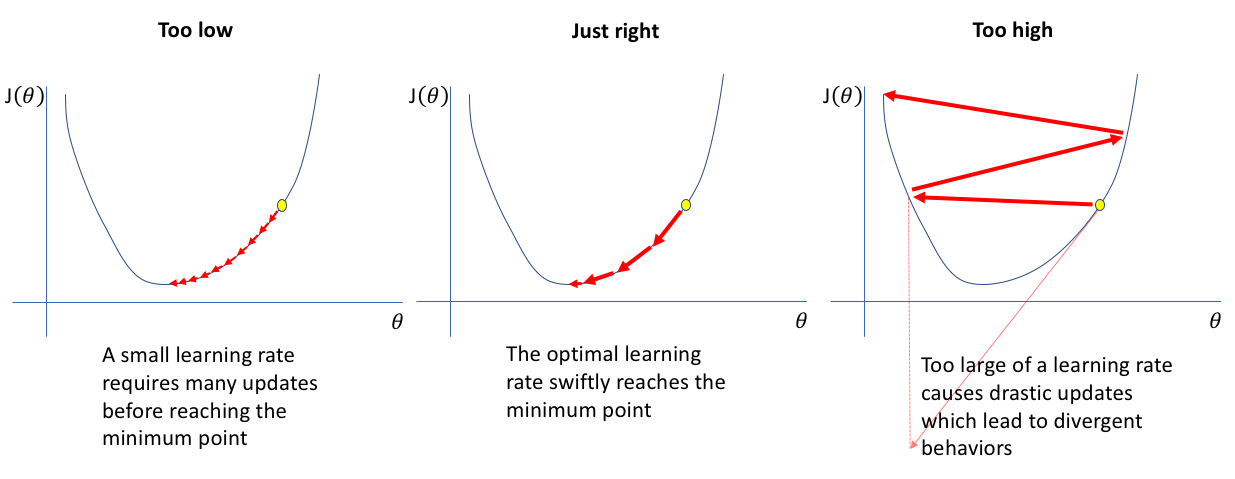
\includegraphics[scale=0.3]{cap5_experimentacion/images/learningRate.png}
    \caption{Tamaño del paso y evolución de la búsqueda según el valor del \textit{learning rate} Fuente:~\cite{learningRateImage}.}
    \label{fig:learningRate}
\end{figure}

Los experimentos explicados a continuación son de 1 iteración de 500 episodios y tienen la misma configuración que el experimento anterior (\nameref{EPS1}). La configuración se muestra en la  Fig.~\ref{fig:dim5_EPS1}. \\

El número óptimo de acciones que se pueden hacer para alcanzar el objetivo sigue siendo 8.

\subsubsection{EPS2\_LR1: Learning rate 0.001} \label{EPS2_LR1}

En este experimento se ha empleado un learning rate con valor de \textbf{0.001}. 

\paragraph{Análisis de las acciones realizadas} 

Como se puede observar en la Fig.~\ref{fig:dim5_lr0.001_ep0.2_acciones}, el número de acciones durante todo el experimento se ha mantenido estable en el valor máximo de acciones permitidas, en concreto 60. Esto implica que no se ha llegado a ninguna solución ya que no ha podido encontrar la función adecuada de aprendizaje. Lo mismo se puede apreciar en el boxplot de la Fig.~\ref{fig:dim5_lr0.001_ep0.2_boxplot}, donde se muestra que la distribución de las acciones se concentra en el valor 60. \\

\begin{figure}
    \centering
    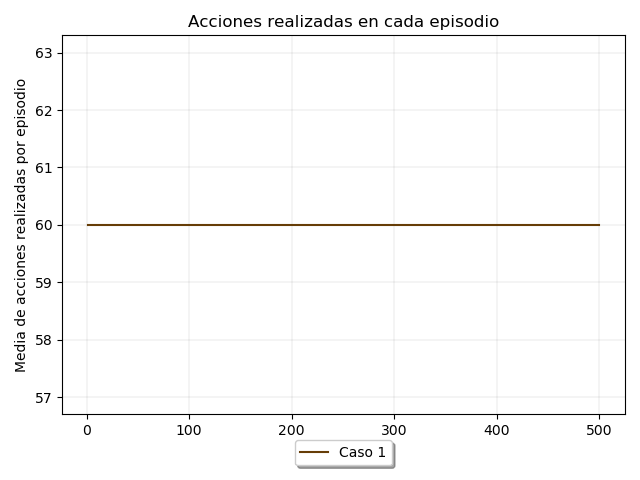
\includegraphics[scale=0.4]{cap5_experimentacion/images/dim5_lr0.001_ep0.2_acciones.png}
    \caption{Acciones realizadas por episodio en el experimento \texttt{EPS2\_LR1}}
    \label{fig:dim5_lr0.001_ep0.2_acciones}
\end{figure}

\begin{figure}
    \centering
    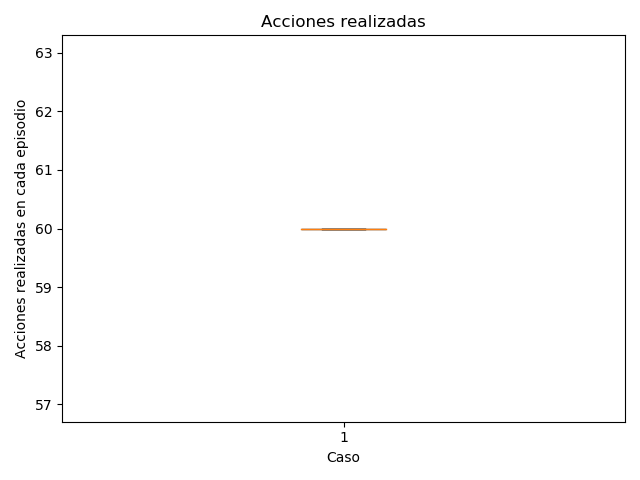
\includegraphics[scale=0.4]{cap5_experimentacion/images/dim5_lr0.001_ep0.2_boxplot.png}
    \caption{Boxplot del experimento \texttt{EPS2\_LR1}.}
    \label{fig:dim5_lr0.001_ep0.2_boxplot}
\end{figure}

Además, como bien era de esperar, no se ha podido encontrar ninguna secuencia de pasos para alcanzar el objetivo. Queda demostrado que para este problema y con estas características concretas, un  \textit{learning rate} bajo no aporta buenos resultados; para que los resultados mejoren, posiblemente sea necesario incrementar el número de pasos que el agente puede realizar para alcanzar el objetivo, ya que supondría que el algoritmo tiene más iteraciones en las que se puede buscar el valor mínimo de la función de pérdida. 

\paragraph{Análisis de las recompensas obtenidas y total de episodios resueltos} 

En cuanto a las recompensas, se muestran en la Fig.~\ref{fig:dim5_lr0.001_ep0.2_recompensa}. Se puede apreciar que a lo largo de la ejecución el agente ha recibido un elevado número de penalizaciones y durante un gran nombre de episodios consecutivos. Sin embargo, se puede observar que en distintas ocasiones el agente ha ido incrementando su recompensa, llegando a valores superiores a 0.6. Es posible que en el caso de que hubiese tenido un número mayor de pasos permitidos por episodio, el agente haya alcanzado su objetivo en algún episodio. \\

\begin{figure}
    \centering
    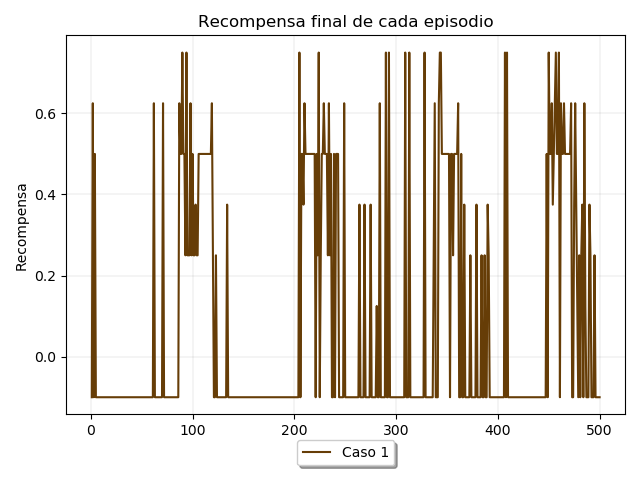
\includegraphics[scale=0.4]{cap5_experimentacion/images/dim5_lr0.001_ep0.2_recompensa.png}
    \caption{Recompensas finales de cada episodio del experimento \texttt{EPS2\_LR1}.}
    \label{fig:dim5_lr0.001_ep0.2_recompensa}
\end{figure}

Como se puede observar en la Fig.~\ref{fig:dim5_lr0.001_ep0.2_porcentajeResuelto}, en este experimento de 500 episodios el agente no ha sido capaz de alcanzar el objetivo.

\begin{figure}
    \centering
    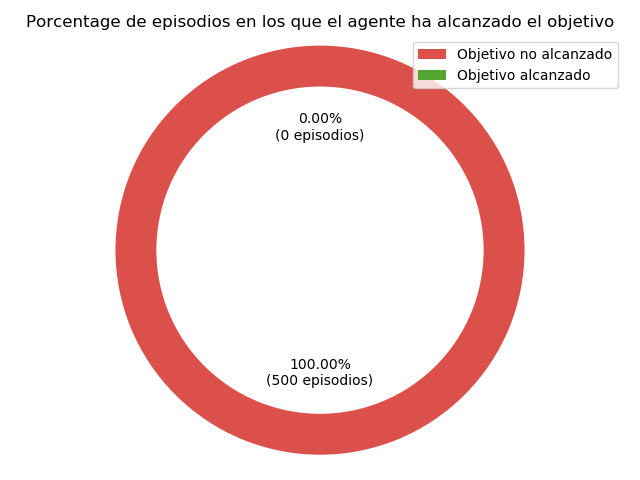
\includegraphics[scale=0.4]{cap5_experimentacion/images/dim5_lr0.001_ep0.2_porcentajeResuelto.png}
    \caption{Porcentaje de episodios en los que el agente alcanza el objetivo en el experimento \texttt{EPS2\_LR1}.}
    \label{fig:dim5_lr0.001_ep0.2_porcentajeResuelto}
\end{figure}

\subsubsection{EPS2\_LR2: Learning rate 0.01} \label{EPS2_LR2}

En este experimento se ha empleado un learning rate con valor de \textbf{0.01}. 

\paragraph{Análisis de las acciones realizadas}

Como bien se puede observar en la Fig.~\ref{fig:dim5_lr0.01_ep0.2_acciones}, la diferencia de resultados obtenidos respecto al experimento anterior (\nameref{EPS2_LR1}) es evidente: el total de acciones realizadas se mantiene en el valor óptimo a lo largo del experimento, con pocos episodios en los que este valor es mayor. \\

\begin{figure}
    \centering
    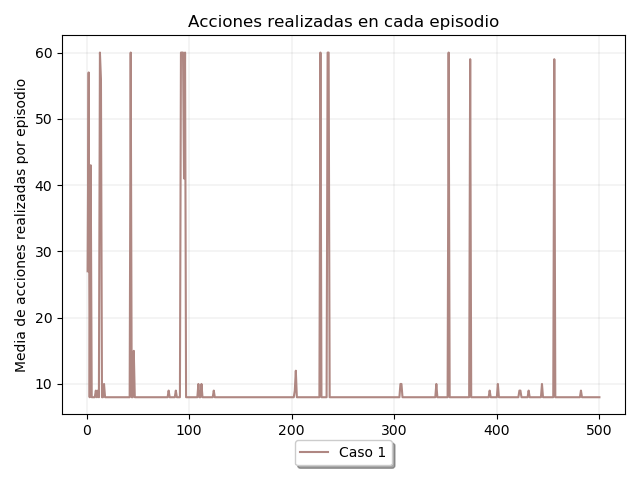
\includegraphics[scale=0.4]{cap5_experimentacion/images/dim5_lr0.01_ep0.2_acciones.png}
        \caption{Acciones realizadas por episodio en el experimento \texttt{EPS2\_LR2}.}
    \label{fig:dim5_lr0.01_ep0.2_acciones}
\end{figure}

Asimismo, el boxplot de la figura Fig.~\ref{fig:dim5_lr0.01_ep0.2_boxplot} muestra que la media de acciones está en el valor óptimo. \\

\begin{figure}
    \centering
    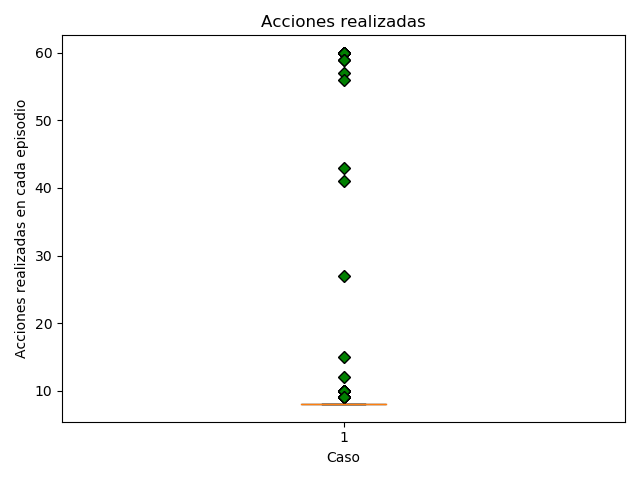
\includegraphics[scale=0.4]{cap5_experimentacion/images/dim5_lr0.01_ep0.2_boxplot.png}
    \caption{Boxplot del experimento \texttt{EPS2\_LR2}.}
    \label{fig:dim5_lr0.01_ep0.2_boxplot}
\end{figure}

En cuanto a las secuencias de acciones realizadas, hay una única acción predominante y se muestra en la Fig.~\ref{fig:dim5_lr0.01_ep0.2_458}. Dicha secuencia se ha aplicado en 458 episodios del total de 500.  \\

\begin{figure}
    \centering
    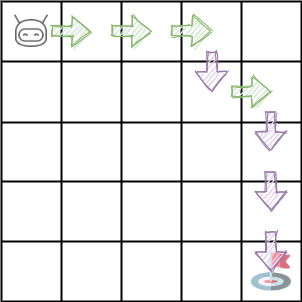
\includegraphics[scale=0.4]{cap5_experimentacion/images/dim5_lr0.01_ep0.2_458.png}
    \caption{Secuencia de acciones realizada en el experimento \texttt{EPS2\_LR2} para llegar al objetivo. Aplicada 458 veces.}
    \label{fig:dim5_lr0.01_ep0.2_458}
\end{figure}

\paragraph{Análisis de las recompensas obtenidas y total de episodios resueltos} 

En cuanto a las recompensas, se muestran en la Fig.~\ref{fig:dim5_lr0.01_ep0.2_recompensa}. Se puede apreciar que a lo largo de la ejecución la recompensa que obtiene el agente se mantiene estable en el valor máximo, con pocos episodios en los que ha recibido penalizaciones.  \\

\begin{figure}
    \centering
    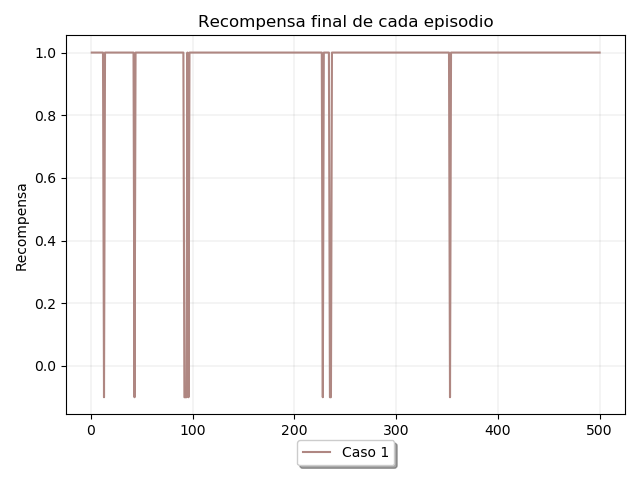
\includegraphics[scale=0.43]{cap5_experimentacion/images/dim5_lr0.01_ep0.2_recompensa.png}
    \caption{Recompensas finales de cada episodio del experimento \texttt{EPS2\_LR2}.}
    \label{fig:dim5_lr0.01_ep0.2_recompensa}
\end{figure}

En este experimento de 500 episodios el agente ha sido capaz de alcanzar el objetivo en 490 episodios. En la Fig.~\ref{fig:dim5_lr0.01_ep0.2_porcentajeResuelto} se observan los porcentajes de episodios resueltos. \\

\begin{figure}
    \centering
    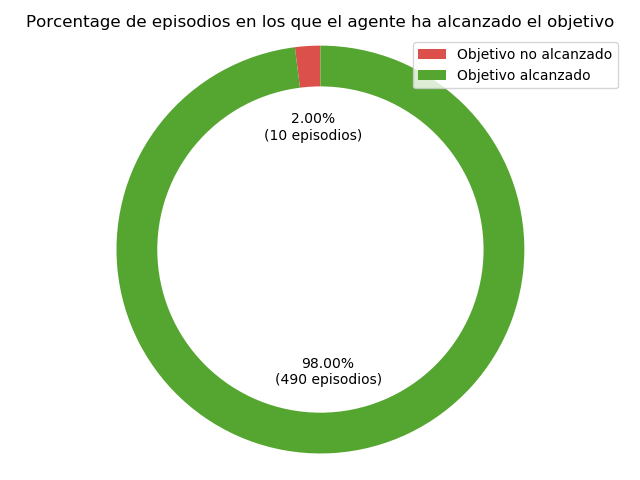
\includegraphics[scale=0.4]{cap5_experimentacion/images/dim5_lr0.01_ep0.2_porcentajeResuelto.png}
    \caption{Porcentaje de episodios en los que el agente alcanza el objetivo en el experimento \texttt{EPS2\_LR2}.}
    \label{fig:dim5_lr0.01_ep0.2_porcentajeResuelto}
\end{figure}

\subsubsection{EPS2\_LR3: Learning rate 0.1} \label{EPS2_LR3}

En este experimento se ha empleado el learning rate con valor de \textbf{0.1}. \\

\paragraph{Análisis de las acciones realizadas}

De la misma manera que ha ocurrido en el experimento \nameref{EPS2_LR1}, las acciones totales realizadas se mantienen estables en el valor máximo permitido, tal como se puede observar en la Fig.~\ref{fig:dim5_lr0.001_ep0.2_acciones} y el boxplot de la Fig.~\ref{fig:dim5_lr0.001_ep0.2_boxplot}. \\

\begin{figure}
    \centering
    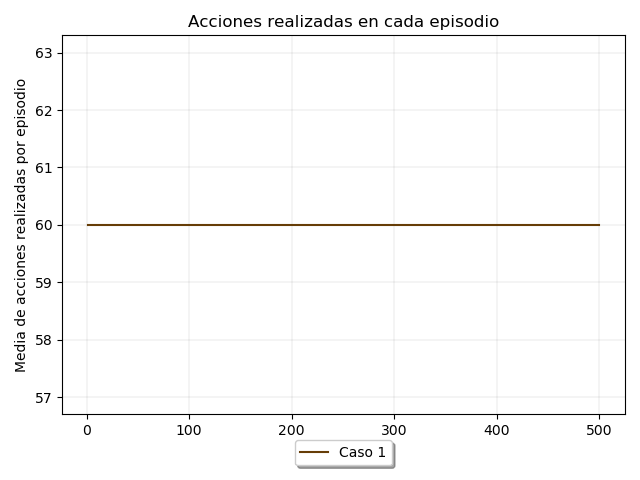
\includegraphics[scale=0.4]{cap5_experimentacion/images/dim5_lr0.001_ep0.2_acciones.png}
   \caption{Acciones realizadas por episodio en el experimento \texttt{EPS2\_LR3}.}
    \label{fig:dim5_lr0.1_ep0.2_acciones}
\end{figure}

\begin{figure}
    \centering
    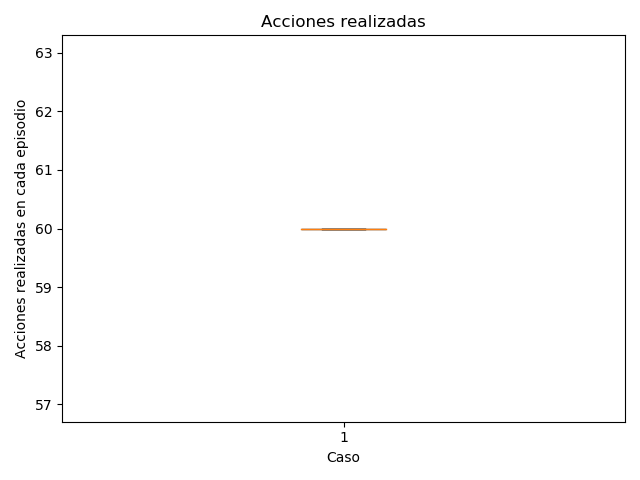
\includegraphics[scale=0.4]{cap5_experimentacion/images/dim5_lr0.001_ep0.2_boxplot.png}
    \caption{Boxplot del experimento \texttt{EPS2\_LR3}.}
    \label{fig:dim5_lr0.1_ep0.2_boxplot}
\end{figure}

En este experimento no ha sido posible detectar ninguna secuencia de acciones que permita al agente alcanzar el objetivo. 

\paragraph{Análisis de las recompensas obtenidas y total de episodios resueltos} 

Por otro lado, respecto a las recompensas obtenidas en el experimento \nameref{EPS2_LR1}, las recompensas de este experimento han sido inferiores. El agente ha recibido constantemente penalizaciones, y en número escaso de episodios ha recibido una recompensa que no superaba el 0.65, aproximadamente.\\

\begin{figure}
    \centering
    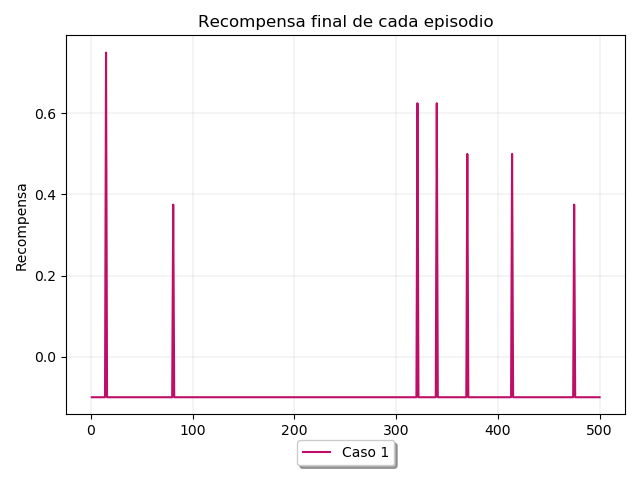
\includegraphics[scale=0.4]{cap5_experimentacion/images/dim5_lr0.1ep0.2_recompensa.png}
    \caption{Recompensas finales de cada episodio del experimento \texttt{EPS2\_LR3}.}
    \label{fig:dim5_lr0.1_ep0.2_recompensa}
\end{figure}

En este experimento de 500 episodios el agente no ha sido capaz de alcanzar el objetivo, tal como se puede observar en la Fig.~\ref{fig:dim5_lr0.1ep0.2_porcentajeResuelto}.

\begin{figure}
    \centering
    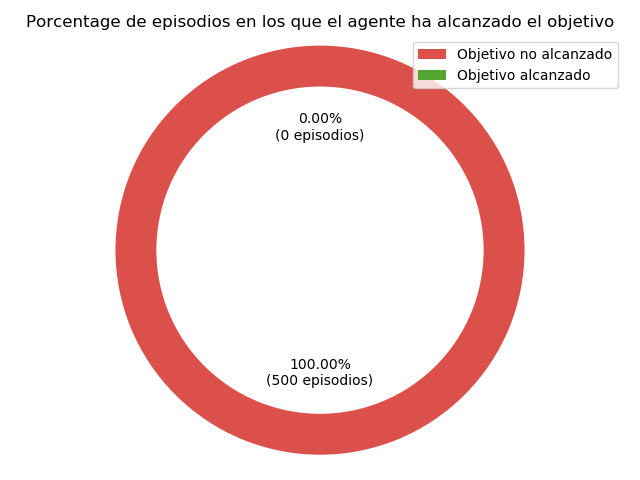
\includegraphics[scale=0.4]{cap5_experimentacion/images/dim5_lr0.1ep0.2_porcentajeResuelto.png}
    \caption{Porcentaje de episodios en los que el agente alcanza el objetivo en el experimento \texttt{EPS2\_LR3}.}
    \label{fig:dim5_lr0.1ep0.2_porcentajeResuelto}
\end{figure}

\subsection{EPS3: Estudio de convergencia  con exploration rate variable} \label{EPS3}

Recordemos que en el apartado de \textbf{\nameref{explorationExploitation}} se ha comentado el dilema de balancear adecuadamente la exploración del entorno y la explotación de los conocimientos ya adquiridos para realizar un aprendizaje eficiente. \\

Este experimento tiene como objetivo observar cómo afecta el \textit{exploration rate}, es decir, la exploración del entorno, al aprendizaje del agente. \\

Los experimentos explicados a continuación son de 1 iteración de 500 episodios y tienen la misma configuración que el experimento anterior (\nameref{EPS1}). La configuración se muestra en la  Fig.~\ref{fig:dim5_EPS1}. \\

El número óptimo de acciones que se pueden hacer para alcanzar el objetivo sigue siendo 8.\\ 


\subsubsection{EPS3\_ER1: Exploration rate 0} \label{EPS3_ER1}

En este experimento el \textit{exploration rate} es de 0, de modo que no se explora el entorno y sólo se emplean los conocimientos ya desarrollados por el agente. Puesto que el agente no ha sido entrenado previamente, intentará alcanzar el objetivo empleando los pesos iniciales de su red interna. 

\paragraph{Análisis de las acciones realizadas}

Como se puede observar en la Fig.~\ref{fig:dim5_lr0.01_ep0_acciones}, el agente ha sido capaz de encontrar el número óptimo de acciones por realizar y ha mantenido de manera relativamente estable este valor a lo largo del experimento; siguen habiendo episodios con el máximo de acciones realizadas, pero comparando con los resultados de los experimentos realizados hasta este punto, se pueden considerar buenos resultados. \\

\begin{figure}
    \centering
    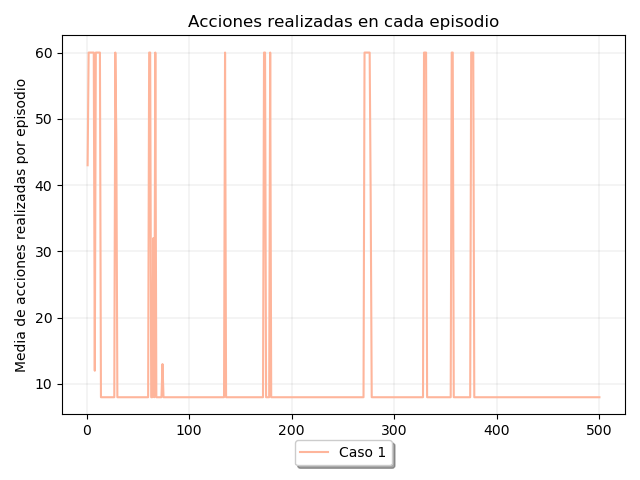
\includegraphics[scale=0.4]{cap5_experimentacion/images/dim5_lr0.01_ep0_acciones.png}
    \caption{Acciones realizadas por episodio en el experimento \texttt{EPS3\_ER1}.}
    \label{fig:dim5_lr0.01_ep0_acciones}
\end{figure}

En el boxplot de la Fig.~\ref{fig:dim5_lr0.01_ep0_boxplot} se muestra la distribución de los datos y se puede observar como la media de las acciones realizadas está en el valor óptimo (8).\\

\begin{figure}
    \centering
    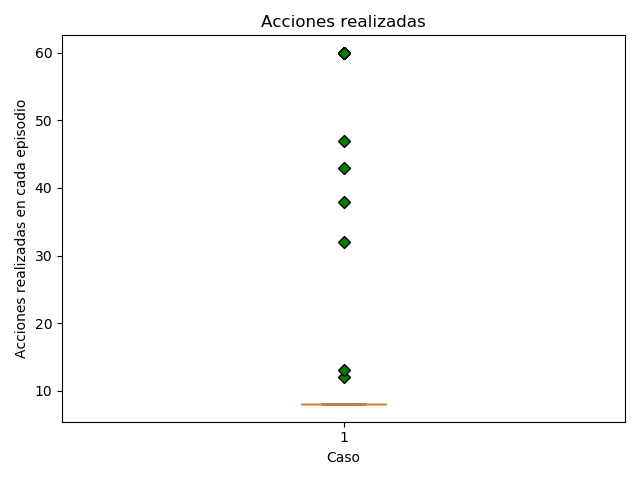
\includegraphics[scale=0.4]{cap5_experimentacion/images/dim5_lr0.01_ep0_boxplot.png}
    \caption{Boxplot del experimento \texttt{EPS3\_ER1}.}
    \label{fig:dim5_lr0.01_ep0_boxplot}
\end{figure}

En la Fig.~\ref{fig:dim5_lr0.01_ep0_453} se puede observar la secuencia de acciones empleada en este experimento para alcanzar el objetivo. De 500 episodios se ha aplicado 453 veces para alcanzar la solución. 

\begin{figure}
    \centering
    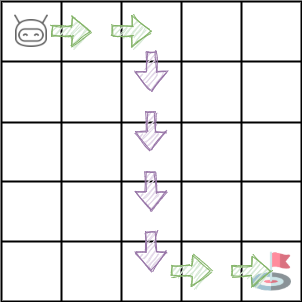
\includegraphics[scale=0.4]{cap5_experimentacion/images/dim5_lr0.01_ep0_453.png}
    \caption{Secuencia de acciones del experimento \texttt{EPS3\_ER1}. Aplicada 453 veces.}
    \label{fig:dim5_lr0.01_ep0_453}
\end{figure}

\paragraph{Análisis de las recompensas obtenidas y total de episodios resueltos} 

En cuanto a las recompensas recibidas en este experimento, se aprecia en la Fig.~\ref{fig:dim5_lr0.01_ep0_recompensa} que se ha mantenido estable alrededor del valor máximo y, además, no ha recibido un número elevado de penalizaciones.  \\

\begin{figure}
    \centering
    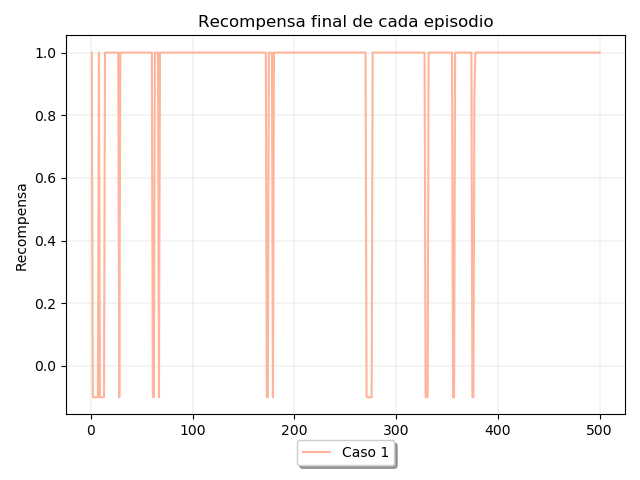
\includegraphics[scale=0.4]{cap5_experimentacion/images/dim5_lr0.01_ep0_recompensa.png}
    \caption{Recompensas finales de cada episodio del experimento \texttt{EPS3\_ER1}.}
    \label{fig:dim5_lr0.01_ep0_recompensa}
\end{figure}

En este experimento de 500 episodios el agente ha sido capaz de alcanzar el objetivo en 468 episodios. En la Fig.~\ref{fig:dim5_lr0.01_ep0_porcentajeResuelto} se muestran los porcentajes de episodios resueltos y no resueltos del experimento. 
\begin{figure}
    \centering
    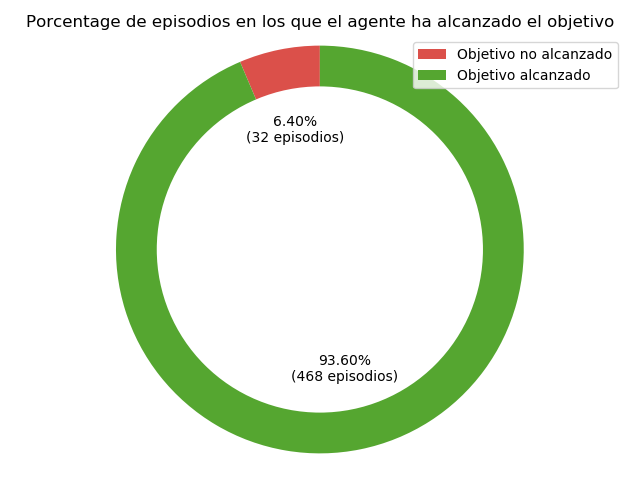
\includegraphics[scale=0.4]{cap5_experimentacion/images/dim5_lr0.01_ep0_porcentajeResuelto.png}
    \caption{Porcentaje de episodios en los que el agente alcanza el objetivo en el experimento \texttt{EPS3\_ER1}.}
    \label{fig:dim5_lr0.01_ep0_porcentajeResuelto}
\end{figure}

\subsubsection{EPS3\_ER2: Exploration rate 0.1} \label{EPS3_ER2}

En este experimento el \textit{exploration rate} es de 0.1, de modo que se explora el entorno el 10\% de las veces y el 90\% restante se emplean los conocimientos ya adquiridos. \\

\paragraph{Análisis de las acciones realizadas}

A diferencia del experimento anterior \nameref{EPS3_ER1}, el agente no consigue alcanzar en ningún momento el valor óptimo de acciones, sino que a lo largo del experimento ha realizado el número máximo de acciones permitido. Dichas recompensas se muestran en la Fig.~\ref{fig:dim5_lr0-01_ep0.1_acciones}. \\

\begin{figure}
    \centering
    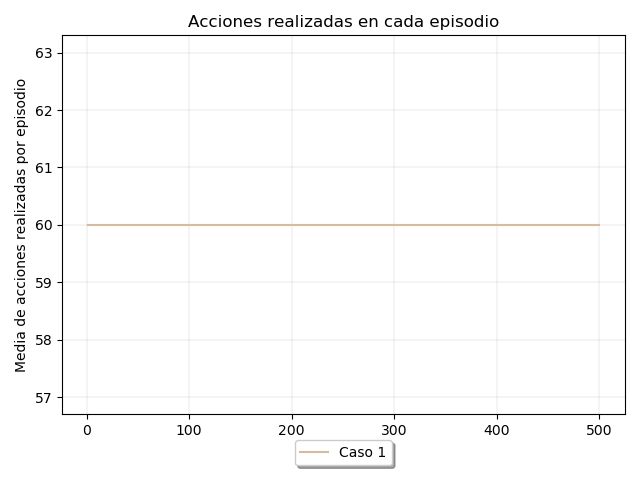
\includegraphics[scale=0.4]{cap5_experimentacion/images/dim5_lr0-01_ep0.1_acciones.png}
    \caption{Acciones realizadas por episodio en el experimento \texttt{EPS3\_ER2}.}
    \label{fig:dim5_lr0-01_ep0.1_acciones}
\end{figure}

En el boxplot de la Fig.~\ref{fig:dim5_lr0-01_ep0.1_boxplot} se aprecia que la distribución de los datos tiene la media en el valor 60.  \\
 
\begin{figure}
    \centering
    \includegraphics[scale=0.4]{cap5_experimentacion/images/dim5_lr0-01_ep0.1_boxplot.png}
    \caption{Boxplot del experimento \texttt{EPS3\_ER2}.}
    \label{fig:dim5_lr0-01_ep0.1_boxplot}
\end{figure}

No se ha conseguido encontrar ninguna secuencia de acciones que lleve al objetivo en este experimento. 

\paragraph{Análisis de las recompensas obtenidas y total de episodios resueltos} 

Tal como se observa en la Fig.~\ref{fig:dim5_lr0-01_ep0.1_recompensa}, las recompensas recibidas a lo largo del experimento son negativas, y las recompensas positivas no superan el 0.6.\\

\begin{figure}
    \centering
    \includegraphics[scale=0.4]{cap5_experimentacion/images/dim5_lr0-01_ep0.1_recompensa.png}
    \caption{Recompensas finales de cada episodio del experimento \texttt{EPS3\_ER2}.}
    \label{fig:dim5_lr0-01_ep0.1_recompensa}
\end{figure}

En este experimento de 500 episodios el agente no ha sido capaz de alcanzar el objetivo tal como se puede observar en la Fig.~\ref{fig:dim5_lr0-01_ep0.1_porcentajeResuelto}. 

\begin{figure}
    \centering
    \includegraphics[scale=0.4]{cap5_experimentacion/images/dim5_lr0-01_ep0.1_porcentajeResuelto.png}
    \caption{Porcentaje de episodios en los que el agente alcanza el objetivo en el experimento \texttt{EPS3\_ER2}.}
    \label{fig:dim5_lr0-01_ep0.1_porcentajeResuelto}
\end{figure}

\subsubsection{EPS3\_ER3: Exploration rate 0.2} \label{EPS3_ER3}

En este experimento el \textit{exploration rate} es de 0.2, un valor que se toma muchas veces por defecto para realizar el aprendizaje. 

\paragraph{Análisis de las acciones realizadas}

Como se puede observar en la Fig.~\ref{fig:dim5_lr0.01_ep0.2_acciones_EPS2_ER3} las acciones realizadas a lo largo del experimento alcanzan mayoritariamente el valor óptimo, con pocos episodios en los que se tome el valor máximo de acciones. \\

\begin{figure}
    \centering
    \includegraphics[scale=0.4]{cap5_experimentacion/images/dim5_lr0.01_ep0.2_acciones.png}
    \caption{Acciones realizadas por episodio en el experimento \texttt{EPS3\_ER3}.}
    \label{fig:dim5_lr0.01_ep0.2_acciones_EPS2_ER3}
\end{figure}

En boxplot de la Fig.~\ref{fig:dim5_lr0.01_ep0.2_boxplot_EPS2_ER3} se puede observar que la media de las acciones realizadas en este experimento está en el valor óptimo. 

\begin{figure}
    \centering
    \includegraphics[scale=0.4]{cap5_experimentacion/images/dim5_lr0.01_ep0.2_boxplot.png}
    \caption{Boxplot del experimento \texttt{EPS3\_ER3}.}
    \label{fig:dim5_lr0.01_ep0.2_boxplot_EPS2_ER3}
\end{figure}

La secuencia de acciones aplicada se muestra en la  Fig.~\ref{fig:dim5_lr0.01_ep0.2_EPS2_ER3}. Se ha aplicado en 458 episodios de 500. 

\begin{figure}
    \centering
    \includegraphics[scale=0.4]{cap5_experimentacion/images/dim5_lr0.01_ep0.2_458.png}
    \caption{Secuencia de acciones encontrada en el experimento \texttt{EPS3\_ER3}. Aplicada 458 veces.}
    \label{fig:dim5_lr0.01_ep0.2_EPS2_ER3}
\end{figure}

\paragraph{Análisis de las recompensas obtenidas y total de episodios resueltos} 

En cuanto a las recompensas, tal como se observa en la Fig.~\ref{fig:dim5_lr0.01_ep0.2_recompensa_EPS3_ER3} se han obtenido valores máximos a lo largo de la ejecución y con un número de penalizaciones bajo. \\
\begin{figure}
    \centering
    \includegraphics[scale=0.4]{cap5_experimentacion/images/dim5_lr0.01_ep0.2_recompensa.png}
    \caption{Recompensas finales de cada episodio del experimento \texttt{EPS3\_ER3}.}
    \label{fig:dim5_lr0.01_ep0.2_recompensa_EPS3_ER3}
\end{figure}

En este experimento de 500 episodios el agente ha sido capaz de alcanzar el objetivo en 490 episodios. En la Fig.~\ref{fig:dim5_lr0.01_ep0.2_porcentajeResuelto} se muestran los porcentajes de episodios resueltos y no resueltos del experimento. 

\begin{figure}
    \centering
    \includegraphics[scale=0.4]{cap5_experimentacion/images/dim5_lr0.01_ep0.2_porcentajeResuelto.png}
    \caption{Porcentaje de episodios en los que el agente alcanza el objetivo en el experimento \texttt{EPS3\_ER3}.}
    \label{fig:dim5_lr0.01_ep0.2_porcentajeResuelto}
\end{figure}

\subsubsection{EPS3\_ER4: Exploration rate 0.3} \label{EPS2_ER4}

En este experimento el \textit{exploration rate} es de 0.3, de modo que se explora el entorno el 30\% de las veces y el 70\% restante se emplean los conocimientos ya adquiridos.

\paragraph{Análisis de las acciones realizadas}

La Fig.~\ref{fig:dim5_lr0.01_ep0.3_acciones} muestra que las acciones realizadas a lo largo del experimento no se han estabilizado por completo, alternando el valor entre óptimo (8) y el máximo (60). \\

\begin{figure}
    \centering
    \includegraphics[scale=0.4]{cap5_experimentacion/images/dim5_lr0.01_ep0.3_acciones.png}
    \caption{Acciones realizadas por episodio en el experimento \texttt{EPS3\_ER4}.}
    \label{fig:dim5_lr0.01_ep0.3_acciones}
\end{figure}

Sin embargo, en el boxplot de la Fig.~\ref{fig:dim5_lr0.01_ep0.3_boxplot} se muestra que la media de la distribución de los datos es igual al número de acciones óptimo, por lo que parece que se ha estabilizado el total de acciones realizadas. \\

\begin{figure}
    \centering
    \includegraphics[scale=0.4]{cap5_experimentacion/images/dim5_lr0.01_ep0.3_boxplot.png}
    \caption{Boxplot del experimento \texttt{EPS3\_ER4}.}
    \label{fig:dim5_lr0.01_ep0.3_boxplot}
\end{figure}

En este experimento se han encontrado 2 secuencias de acciones diferentes: la predominante se ha aplicado 409 veces y se muestra en la Fig.~\ref{fig:dim5_lr0.01_ep0.3_409}; la segunda se ha aplicado 47 veces y se muestra en la Fig.~\ref{fig:dim5_lr0.01_ep0.3_47}. En total se ha alcanzado un número de episodios resueltos similar a los anteriores (456 episodios resueltos de 500).

\begin{figure}
    \centering
    \begin{subfigure}{.5\textwidth}
        \centering
        \includegraphics[scale=0.4]{cap5_experimentacion/images/dim5_lr0.01_ep0.3_409.png}
        \caption{Aplicada 409 veces.}
        \label{fig:dim5_lr0.01_ep0.3_409}
    \end{subfigure}%       
    \begin{subfigure}{.5\textwidth}
        \centering
        \includegraphics[scale=0.4]{cap5_experimentacion/images/dim5_lr0.01_ep0.3_47.png}
        \caption{Aplicada 47 veces.}
        \label{fig:dim5_lr0.01_ep0.3_47}
    \end{subfigure}
    \caption{Secuencias de acciones encontradas en el experimento \texttt{EPS3\_ER4}.}
    \label{fig:dim5_lr0.01_ep0.3}
\end{figure}

\paragraph{Análisis de las recompensas obtenidas y total de episodios resueltos} 

En cuanto a las recompensas, tal como se observa en la Fig.~\ref{fig:dim5_lr0.01_ep0.3_recompensa} se han obtenido valores máximos a lo largo de la ejecución y con un número de penalizaciones medio pero aceptables. Hay que recordar que es normal que el agente cometa algún error ya que aún está aprendiendo. \\

\begin{figure}
    \centering
    \includegraphics[scale=0.4]{cap5_experimentacion/images/dim5_lr0.01_ep0.3_recompensa.png}
    \caption{Recompensas finales de cada episodio del experimento \texttt{EPS3\_ER4}.}
    \label{fig:dim5_lr0.01_ep0.3_recompensa}
\end{figure}

En este experimento de 500 episodios el agente ha sido capaz de alcanzar el objetivo en 482 episodios. En la Fig.~\ref{fig:dim5_lr0.01_ep0.3_porcentajeResuelto} se muestran los porcentajes de episodios resueltos y no resueltos del experimento.

\begin{figure}
    \centering
    \includegraphics[scale=0.4]{cap5_experimentacion/images/dim5_lr0.01_ep0.3_porcentajeResuelto.png}
    \caption{Porcentaje de episodios en los que el agente alcanza el objetivo en el experimento \texttt{EPS3\_ER4}.}
    \label{fig:dim5_lr0.01_ep0.3_porcentajeResuelto}
\end{figure}

\subsubsection{EPS3\_ER5: Exploration rate 0.4} \label{EPS3_ER5}

En este experimento el \textit{exploration rate} es de 0.4, de modo que se explora el entorno el 40\% de las veces y el 60\% restante se emplean los conocimientos ya adquiridos. \\

\paragraph{Análisis de las acciones realizadas}

Las acciones realizadas en cada episodio se estabilizan en el valor máximo permitido, tal como se observa en la Fig.~\ref{fig:dim5_lr0.01_ep0.4_acciones}. \\

\begin{figure}
    \centering
    \includegraphics[scale=0.4]{cap5_experimentacion/images/dim5_lr0.01_ep0.4_acciones.png}
    \caption{Acciones realizadas por episodio en el experimento \texttt{EPS3\_ER5}.}
    \label{fig:dim5_lr0.01_ep0.4_acciones}
\end{figure}

En el boxplot de la Fig.~\ref{fig:dim5_lr0.01_ep0.4_boxplot} se observa que la media de las acciones realizada tiene el valor 60, el número máximo de acciones permitidas. \\

\begin{figure}
    \centering
    \includegraphics[scale=0.4]{cap5_experimentacion/images/dim5_lr0.01_ep0.4_boxplot.png}
    \caption{Boxplot del experimento \texttt{EPS3\_ER5}.}
    \label{fig:dim5_lr0.01_ep0.4_boxplot}
\end{figure}

En cuanto a las secuencias de acciones, no se ha encontrado ninguna que permita al agente alcanzar el objetivo. 

\paragraph{Análisis de las recompensas obtenidas y total de episodios resueltos} 

La recompensa obtenida a lo largo del experimento se encuentra por debajo del cero y, además, se le ha penalizado el agente en episodios consecutivos. En la Fig.~\ref{fig:dim5_lr0.01_ep0.4_recompensa} se aprecian dichas recompensas. \\

\begin{figure}
    \centering
    \includegraphics[scale=0.4]{cap5_experimentacion/images/dim5_lr0.01_ep0.4_recompensa.png}
    \caption{Recompensas finales de cada episodio del experimento \texttt{EPS3\_ER5}.}
    \label{fig:dim5_lr0.01_ep0.4_recompensa}
\end{figure}

En este experimento de 500 episodios el agente ha sido capaz de alcanzar el objetivo en un sólo episodio. En la Fig.~\ref{fig:dim5_lr0.01_ep0.4_porcentajeResuelto} se muestran los porcentajes de episodios resueltos y no resueltos del experimento. 

\begin{figure}
    \centering
    \includegraphics[scale=0.4]{cap5_experimentacion/images/dim5_lr0.01_ep0.4_porcentajeResuelto.png}
    \caption{Porcentaje de episodios en los que el agente alcanza el objetivo en el experimento \texttt{EPS3\_ER5}.}
    \label{fig:dim5_lr0.01_ep0.4_porcentajeResuelto}
\end{figure}

\subsubsection{EPS3\_ER6: Exploration rate 0.5} \label{EPS3_ER6}

En este experimento el \textit{exploration rate} es de 0.5, de modo que se explora el entorno la mitad de las veces y la otra mitad restante se emplean los conocimientos ya adquiridos. \\

\paragraph{Análisis de las acciones realizadas}

En la Fig.~\ref{fig:dim5_lr0.01_ep0.5_acciones} se muestra el número total de acciones por episodio realizado a lo largo del experimento. Dichas acciones se estabilizan en el valor máximo permitido, teniendo en el inicio del experimento unos episodios en los que sí que se ha alcanzado el valor óptimo. \\

\begin{figure}
    \centering
    \includegraphics[scale=0.4]{cap5_experimentacion/images/dim5_lr0.01_ep0.5_acciones.png}
    \caption{Acciones realizadas por episodio en el experimento \texttt{EPS3\_ER6}.}
    \label{fig:dim5_lr0.01_ep0.5_acciones}
\end{figure}

El boxplot de la Fig.~\ref{fig:dim5_lr0.01_ep0.5_boxplot} muestra que la media de las acciones realizadas es de 60 acciones. \\
\begin{figure}
    \centering
    \includegraphics[scale=0.4]{cap5_experimentacion/images/dim5_lr0.01_ep0.5_boxplot.png}
    \caption{Boxplot del experimento \texttt{EPS3\_ER6}.}
    \label{fig:dim5_lr0.01_ep0.5_boxplot}
\end{figure}

Aunque haya tenido tan malos resultados, el agente ha sido capaz de alcanzar su objetivo siguiendo 2 secuencias de acciones. Dichas secuencias se muestran en la Fig.~\ref{fig:dim5_lr0.01_ep0.5_6}. Ambas se han aplicado en 6 episodios distintos del experimento.  \\ 
\begin{figure}
    \centering
    \begin{subfigure}{.5\textwidth}
        \centering
        \includegraphics[scale=0.4]{cap5_experimentacion/images/dim5_lr0.01_ep0.5_6_1.png}
        \caption{Aplicada 6 veces.}
        \label{fig:dim5_lr0.01_ep0.5_6_1}
    \end{subfigure}%       
    \begin{subfigure}{.5\textwidth}
        \centering
        \includegraphics[scale=0.4]{cap5_experimentacion/images/dim5_lr0.01_ep0.5_6_2.png}
        \caption{Aplicada 6 veces.}
        \label{fig:dim5_lr0.01_ep0.5_6_2}
    \end{subfigure}
    \caption{Secuencias de acciones seguidas en el experimento \texttt{EPS3\_ER6}.}
    \label{fig:dim5_lr0.01_ep0.5_6}
\end{figure}

\paragraph{Análisis de las recompensas obtenidas y total de episodios resueltos} 

Sin embargo, como bien se ha mencionado anteriormente, al principio del experimento el agente ha recibido recompensas máximas en varios episodios. El resto del experimento recibe penalizaciones, pero son menos frecuentes que en el experimento \nameref{EPS3_ER5}. \\

\begin{figure}
    \centering
    \includegraphics[scale=0.4]{cap5_experimentacion/images/dim5_lr0.01_ep0.5_recompensa.png}
    \caption{Recompensas finales de cada episodio del experimento \texttt{EPS3\_ER6}.}
    \label{fig:dim5_lr0.01_ep0.5_recompensa}
\end{figure}

En este experimento de 500 episodios el agente ha sido capaz de alcanzar el objetivo en 21 episodios. En la Fig.~\ref{fig:dim5_lr0.01_ep0.5_porcentajeResuelto} se muestran los porcentajes de episodios resueltos y no resueltos del experimento.

\begin{figure}
    \centering
    \includegraphics[scale=0.4]{cap5_experimentacion/images/dim5_lr0.01_ep0.5_porcentajeResuelto.png}
    \caption{Porcentaje de episodios en los que el agente alcanza el objetivo en el experimento \texttt{EPS3\_ER6}.}
    \label{fig:dim5_lr0.01_ep0.5_porcentajeResuelto}
\end{figure}

\subsubsection{EPS3\_ER7: Exploration rate 0.6} \label{EPS3_ER7}

En este experimento el \textit{exploration rate} es de 0.6, de modo que se explora el 60\% las veces y en el 40\% restante se emplean los conocimientos ya adquiridos. \\

\paragraph{Análisis de las acciones realizadas}

El total de acciones realizadas vuelven a estabilizarse en el valor máximo permitido tal como se muestra en la Fig.~\ref{fig:dim5_lr0.01_ep0.6_acciones}. \\

\begin{figure}
    \centering
    \includegraphics[scale=0.4]{cap5_experimentacion/images/dim5_lr0.01_ep0.6_acciones.png}
    \caption{Acciones realizadas por episodio en el experimento \texttt{EPS3\_ER7}.}
    \label{fig:dim5_lr0.01_ep0.6_acciones}
\end{figure}

En la Fig.~\ref{fig:dim5_lr0.01_ep0.6_boxplot} se muestra que la media de acciones es de 60. \\ 

\begin{figure}
    \centering
    \includegraphics[scale=0.4]{cap5_experimentacion/images/dim5_lr0.01_ep0.6_boxplot.png}
    \caption{Boxplot del experimento \texttt{EPS3\_ER7}.}
    \label{fig:dim5_lr0.01_ep0.6_boxplot}
\end{figure}

No se ha encontrado ninguna secuencia de acciones que lleven al agente al objetivo.

\paragraph{Análisis de las recompensas obtenidas y total de episodios resueltos} 

En cuanto a las recompensas mostradas en la Fig.~\ref{fig:dim5_lr0.01_ep0.6_recompensa}, se puede decir que son las peores recompensas que se han obtenido de todos los experimentos realizados ya que las penalizaciones son secuenciales casi en la totalidad de los episodios. \\

\begin{figure}
    \centering
    \includegraphics[scale=0.4]{cap5_experimentacion/images/dim5_lr0.01_ep0.6_recompensa.png}
    \caption{Recompensas finales de cada episodio del experimento \texttt{EPS3\_ER7}.}
    \label{fig:dim5_lr0.01_ep0.6_recompensa}
\end{figure}

En este experimento de 500 episodios el agente no ha sido capaz de alcanzar el objetivo tal como se muestra en la Fig.~\ref{fig:dim5_lr0.01_ep0.6_porcentajeResuelto}.

\begin{figure}
    \centering
    \includegraphics[scale=0.4]{cap5_experimentacion/images/dim5_lr0.01_ep0.6_porcentajeResuelto.png}
    \caption{Porcentaje de episodios en los que el agente alcanza el objetivo en el experimento \texttt{EPS3\_ER7}.}
    \label{fig:dim5_lr0.01_ep0.6_porcentajeResuelto}
\end{figure}

\subsubsection{EPS3\_ER8: Exploration rate 0.7} \label{EPS2_ER8}

En este experimento el \textit{exploration rate} es de 0.7, de modo que se explora el 70\% las veces y en el 30\% restante se emplean los conocimientos ya adquiridos. \\

\paragraph{Análisis de acciones realizadas}

La Fig.~\ref{fig:dim5_lr0.01_ep0.7_acciones} muestra las acciones realizadas en cada episodio; respecto a los experimentos anteriores, se puede observar que los resultados obtenidos en este experimento son los mejores, ya que el número total de acciones realizadas en los episodios son estables entorno al valor óptimo. \\

\begin{figure}
    \centering
    \includegraphics[scale=0.4]{cap5_experimentacion/images/dim5_lr0.01_ep0.7_acciones.png}
    \caption{Acciones realizadas por episodio en el experimento \texttt{EPS3\_ER8}.}
    \label{fig:dim5_lr0.01_ep0.7_acciones}
\end{figure}

El boxplot de la Fig.~\ref{fig:dim5_lr0.01_ep0.7_boxplot} nos muestra que, además, el total de acciones tomadas en cada episodio a lo largo de la ejecución tiene una media de 8. \\

\begin{figure}
    \centering
    \includegraphics[scale=0.4]{cap5_experimentacion/images/dim5_lr0.01_ep0.7_boxplot.png}
    \caption{Boxplot del experimento \texttt{EPS3\_ER8}.}
    \label{fig:dim5_lr0.01_ep0.7_boxplot}
\end{figure}

En este experimento se han encontrado 6 secuencias distintas de acciones que se han realizado para alcanzar el objetivo. La secuencia predominante es la que se muestra en la Fig.~\ref{fig:dim5_lr0.01_ep0.7_174}, con un total de 174 episodios en los que se ha aplicado. \\
\begin{figure}
    \centering
    \begin{subfigure}{.3\textwidth}
        \centering
        \includegraphics[scale=0.35]{cap5_experimentacion/images/dim5_lr0.01_ep0.7_174.png}
        \caption{Aplicada 174 veces.}
        \label{fig:dim5_lr0.01_ep0.7_174}
    \end{subfigure}%       
    \begin{subfigure}{.3\textwidth}
        \centering
        \includegraphics[scale=0.35]{cap5_experimentacion/images/dim5_lr0.01_ep0.7_139.png}
        \caption{Aplicada 139 veces.}
        \label{fig:dim5_lr0.01_ep0.7_139}
    \end{subfigure}%
    \begin{subfigure}{.3\textwidth}
        \centering
        \includegraphics[scale=0.35]{cap5_experimentacion/images/dim5_lr0.01_ep0.7_88.png}
        \caption{Aplicada 88 veces.}
        \label{fig:dim5_lr0.01_ep0.7_88}
    \end{subfigure}
    \begin{subfigure}{.3\textwidth}
        \centering
        \includegraphics[scale=0.35]{cap5_experimentacion/images/dim5_lr0.01_ep0.7_32.png}
        \caption{Aplicada 32 veces.}
        \label{fig:dim5_lr0.01_ep0.7_32}
    \end{subfigure}%       
    \begin{subfigure}{.3\textwidth}
        \centering
        \includegraphics[scale=0.35]{cap5_experimentacion/images/dim5_lr0.01_ep0.7_30.png}
        \caption{Aplicada 30 veces.}
        \label{fig:dim5_lr0.01_ep0.7_30}
    \end{subfigure}%
    \begin{subfigure}{.3\textwidth}
        \centering
        \includegraphics[scale=0.35]{cap5_experimentacion/images/dim5_lr0.01_ep0.7_7.png}
        \caption{Aplicada 7 veces.}
        \label{fig:dim5_lr0.01_ep0.7_7}
    \end{subfigure}
    \caption{Secuencias de acciones seguidas en el experimento \texttt{EPS3\_ER8}}
    \label{fig:dim5_lr0.01_ep0.7}
\end{figure}


\paragraph{Análisis de las recompensas obtenidas y total de episodios resueltos} 

En cuanto a la recompensa mostrada en la Fig.~\ref{fig:dim5_lr0.01_ep0.7_recompensa}, se observa que es máxima a lo largo de toda la ejecución con la excepción de una única penalización recibida. \\

\begin{figure}
    \centering
    \includegraphics[scale=0.4]{cap5_experimentacion/images/dim5_lr0.01_ep0.7_recompensa.png}
    \caption{Recompensas finales de cada episodio del experimento \texttt{EPS3\_ER8}.}
    \label{fig:dim5_lr0.01_ep0.7_recompensa}
\end{figure}

En este experimento de 500 episodios el agente ha sido capaz de alcanzar el objetivo en 496 episodios. En la Fig.~\ref{fig:dim5_lr0.01_ep0.7_porcentajeResuelto} se muestran los porcentajes de episodios resueltos y no resueltos del experimento. 

\begin{figure}
    \centering
    \includegraphics[scale=0.4]{cap5_experimentacion/images/dim5_lr0.01_ep0.7_porcentajeResuelto.png}
    \caption{Porcentaje de episodios en los que el agente alcanza el objetivo en el experimento \texttt{EPS3\_ER8}.}
    \label{fig:dim5_lr0.01_ep0.7_porcentajeResuelto}
\end{figure}

\subsubsection{EPS3\_ER9: Exploration rate 0.8} \label{EPS2_ER9}

En este experimento el \textit{exploration rate} es de 0.8, de modo que se explora el 80\% las veces y en el 20\% restante se emplean los conocimientos ya adquiridos. \\

\paragraph{Análisis de las acciones realizadas}

En este experimento el total de acciones realizadas vuelven a estabilizarse en el valor máximo permitido. En la Fig.~\ref{fig:dim5_lr0.01_ep0.8_acciones} se aprecia la evolución a lo largo del experimento. \\

\begin{figure}
    \centering
    \includegraphics[scale=0.4]{cap5_experimentacion/images/dim5_lr0.01_ep0.8_acciones.png}
        \caption{Acciones realizadas por episodio en el experimento \texttt{EPS3\_ER9}.}
    \label{fig:dim5_lr0.01_ep0.8_acciones}
\end{figure}

En el boxplot de la Fig.~\ref{fig:dim5_lr0.01_ep0.8_boxplot} se puede ver que la media de las acciones realizadas es de 60.

\begin{figure}
    \centering
    \includegraphics[scale=0.4]{cap5_experimentacion/images/dim5_lr0.01_ep0.8_boxplot.png}
    \caption{Boxplot del experimento \texttt{EPS3\_ER9}.}
    \label{fig:dim5_lr0.01_ep0.8_boxplot}
\end{figure}

\paragraph{Análisis de las recompensas obtenidas y total de episodios resueltos} 

Las recompensas, mostradas en la la Fig.~\ref{fig:dim5_lr0.01_ep0.8_recompensa}, han sido mayoritariamente negativas. \\

\begin{figure}
    \centering
    \includegraphics[scale=0.4]{cap5_experimentacion/images/dim5_lr0.01_ep0.8_recompensa.png}
    \caption{Recompensas finales de cada episodio del experimento \texttt{EPS3\_ER9}.}
    \label{fig:dim5_lr0.01_ep0.8_recompensa}
\end{figure}

En este experimento de 500 episodios el agente ha sido capaz de alcanzar el objetivo en un único episodio, tal como se aprecia en la Fig.~\ref{fig:dim5_lr0.01_ep0.8_porcentajeResuelto}. 

\begin{figure}
    \centering
    \includegraphics[scale=0.4]{cap5_experimentacion/images/dim5_lr0.01_ep0.8_porcentajeResuelto.png}
    \caption{Porcentaje de episodios en los que el agente alcanza el objetivo en el experimento \texttt{EPS3\_ER9}.}
    \label{fig:dim5_lr0.01_ep0.8_porcentajeResuelto}
\end{figure}

\subsubsection{EPS3\_ER10: Exploration rate 0.9}

En este experimento el \textit{exploration rate} es de 0.9, de modo que se explora el 90\% las veces y en el 10\% restante se emplean los conocimientos ya adquiridos.

\paragraph{Análisis de las acciones realizadas}

La Fig.~\ref{fig:dim5_lr0.01_ep0.9_acciones} muestra las acciones realizadas en cada episodio. El número de acciones realizados por episodio se ha estabilizado en el valor óptimo. \\

\begin{figure}
    \centering
    \includegraphics[scale=0.4]{cap5_experimentacion/images/dim5_lr0.01_ep0.9_acciones.png}
    \caption{Acciones realizadas por episodio en el experimento \texttt{EPS3\_ER10}.}
    \label{fig:dim5_lr0.01_ep0.9_acciones}
\end{figure}

El boxplot de la Fig.~\ref{fig:dim5_lr0.01_ep0.9_boxplot} muestra que la media es equivalente al valor óptimo, es decir, a 8. \\

\begin{figure}
    \centering
    \includegraphics[scale=0.4]{cap5_experimentacion/images/dim5_lr0.01_ep0.9_boxplot.png}
    \caption{Boxplot del experimento \texttt{EPS3\_ER10}.}
    \label{fig:dim5_lr0.01_ep0.9_boxplot}
\end{figure}
 
Se han encontrado 3 secuencias de acciones y se muestran en la Fig.~\ref{fig:dim5_lr0.01_ep0.9}. La secuencia predominante (Fig.~\ref{fig:dim5_lr0.01_ep0.9_383})se ha aplicado 383 veces. \\

\begin{figure}
    \centering
    \begin{subfigure}{.3\textwidth}
        \centering
        \includegraphics[scale=0.35]{cap5_experimentacion/images/dim5_lr0.01_ep0.9_383.png}
        \caption{Aplicada 383 veces.}
        \label{fig:dim5_lr0.01_ep0.9_383}
    \end{subfigure}%       
    \begin{subfigure}{.3\textwidth}
        \centering
        \includegraphics[scale=0.35]{cap5_experimentacion/images/dim5_lr0.01_ep0.9_55.png}
        \caption{Aplicada 55 veces.}
        \label{fig:dim5_lr0.01_ep0.9_55}
    \end{subfigure}%
    \begin{subfigure}{.3\textwidth}
        \centering
        \includegraphics[scale=0.35]{cap5_experimentacion/images/dim5_lr0.01_ep0.9_9.png}
        \caption{Aplicada 9 veces.}
        \label{fig:dim5_lr0.01_ep0.9_9}
    \end{subfigure}
    \caption{Secuencias de acciones seguidas en el experimento \texttt{EPS3\_ER10}.}
    \label{fig:dim5_lr0.01_ep0.9}
\end{figure}

\paragraph{Análisis de las recompensas obtenidas y total de episodios resueltos} 
 
En cuanto a las recompensas, tal como se muestran en la Fig.~\ref{fig:dim5_lr0.01_ep0.9_recompensa}, han sido máximas a lo largo del experimento menos en unos pocos episodios en los que el agente ha recibido recompensas negativas. \\
 
\begin{figure}
    \centering
    \includegraphics[scale=0.4]{cap5_experimentacion/images/dim5_lr0.01_ep0.9_recompensa.png}
    \caption{Recompensas finales de cada episodio del experimento \texttt{EPS3\_ER10}.}
    \label{fig:dim5_lr0.01_ep0.9_recompensa}
\end{figure}

En este experimento de 500 episodios, el agente ha sido capaz de alcanzar el objetivo en 481 episodios. En la Fig.~\ref{fig:dim5_lr0.01_ep0.9_porcentajeResuelto} se muestran los porcentajes de episodios resueltos y no resueltos del experimento. \\

\begin{figure}
    \centering
    \includegraphics[scale=0.4]{cap5_experimentacion/images/dim5_lr0.01_ep0.9_porcentajeResuelto.png}
    \caption{Porcentaje de episodios en los que el agente alcanza el objetivo en el experimento \texttt{EPS3\_ER10}.}
    \label{fig:dim5_lr0.01_ep0.9_porcentajeResuelto}
\end{figure}

\subsubsection{EPS3\_ER11: Exploration rate 1}

Y, por último, en este experimento el \textit{exploration rate} es de 1, de modo que se explora siempre el entorno y no se emplea nunca el conocimiento adquirido de las experiencias anteriores. 

\paragraph{Análisis de las acciones realizadas}

La Fig.~\ref{fig:dim5_lr0.01_ep1_acciones} muestra que las acciones realizadas a lo largo de la ejecución han sido relativamente estables alrededor del valor óptimo (8).\\

\begin{figure}
    \centering
    \includegraphics[scale=0.4]{cap5_experimentacion/images/dim5_lr0.01_ep1_acciones.png}
    \caption{Acciones realizadas por episodio en el experimento \texttt{EPS3\_ER11}.}
    \label{fig:dim5_lr0.01_ep1_acciones}
\end{figure}

El boxplot de la Fig.~\ref{fig:dim5_lr0.01_ep1_boxplot} muestra que la media es equivalente al valor óptimo, es decir, a 8. \\

\begin{figure}
    \centering
    \includegraphics[scale=0.4]{cap5_experimentacion/images/dim5_lr0.01_ep1_boxplot.png}
    \caption{Boxplot del experimento \texttt{EPS3\_ER11}.}
    \label{fig:dim5_lr0.01_ep1_boxplot}
\end{figure}

Se han encontrado 4 secuencias de acciones diferentes para alcanzar el objetivo. Se muestran en la Fig.~\ref{fig:dim5_lr0.01_ep1}.

\begin{figure}
    \centering
    \begin{subfigure}{.5\textwidth}
        \centering
        \includegraphics[scale=0.4]{cap5_experimentacion/images/dim5_lr0.01_ep1_203.png}
        \caption{Aplicada 203 veces.}
        \label{fig:dim5_lr0.01_ep1_203}
    \end{subfigure}%       
    \begin{subfigure}{.5\textwidth}
        \centering
        \includegraphics[scale=0.4]{cap5_experimentacion/images/dim5_lr0.01_ep1_153.png}
        \caption{Aplicada 153 veces.}
        \label{fig:dim5_lr0.01_ep1_153}
    \end{subfigure}
    \begin{subfigure}{.5\textwidth}
        \centering
        \includegraphics[scale=0.4]{cap5_experimentacion/images/dim5_lr0.01_ep1_51.png}
        \caption{Aplicada 51 veces.}
        \label{fig:dim5_lr0.01_ep1_51}
    \end{subfigure}%       
    \begin{subfigure}{.5\textwidth}
        \centering
        \includegraphics[scale=0.4]{cap5_experimentacion/images/dim5_lr0.01_ep1_43.png}
        \caption{Aplicada 43 veces.}
        \label{fig:dim5_lr0.01_ep1_43}
    \end{subfigure}
    \caption{Secuencias de acciones seguidas en el experimento \texttt{EPS3\_ER11}.}
    \label{fig:dim5_lr0.01_ep1}
\end{figure}

\paragraph{Análisis de las recompensas obtenidas y total de episodios resueltos} 

En cuanto a las recompensas, tal como se muestran en la Fig.~\ref{fig:dim5_lr0.01_ep1_recompensa}, han sido máximas a lo largo del experimento menos en unos pocos episodios en los que el agente ha recibido una penalización. \\
  
\begin{figure}
    \centering
    \includegraphics[scale=0.4]{cap5_experimentacion/images/dim5_lr0.01_ep1_recompensa.png}
    \caption{Recompensas finales de cada episodio del experimento \texttt{EPS3\_ER11}.}
    \label{fig:dim5_lr0.01_ep1_recompensa}
\end{figure}

En este experimento de 500 episodios, el agente ha sido capaz de alcanzar el objetivo en 485 episodios. En la Fig.~\ref{fig:dim5_lr0.01_ep1_porcentajeResuelto} se muestran los porcentajes de episodios resueltos y no resueltos del experimento. 

\begin{figure}
    \centering
    \includegraphics[scale=0.4]{cap5_experimentacion/images/dim5_lr0.01_ep1_porcentajeResuelto.png}
    \caption{Porcentaje de episodios en los que el agente alcanza el objetivo en el experimento \texttt{EPS3\_ER11}.}
    \label{fig:dim5_lr0.01_ep1_porcentajeResuelto}
\end{figure}

\subsection{CHG\_ORG: Alternando el inicio del agente en un entorno 5x5} \label{CHG_ORG}

Este experimento se ha separado en dos partes diferentes: en la primera parte se realiza la ejecución original y, en la segunda, se aplican variaciones en la configuración del entorno para observar si los resultados obtenidos cambian respecto a los resultados de la ejecución original. 

\subsubsection{Experimento original}

Este experimento se ha realizado con 3 iteraciones de 300 episodios cada. Las posición inicial del agente se ha ido variando y la del posición del objetivo ha sido en (4, 4). Se ha empleado el modelo del agente obtenido en el experimento anterior \nameref{EPS1}, es decir, la red está ajustada con los pesos obtenidos a partir de la realización de este experimento en concreto. \\


En la Fig.~\ref{fig:chg_org_config} se puede visualizar el entorno del problema con las configuraciones de cada iteración. \\

\begin{figure}
    \centering
    \begin{subfigure}{.35\textwidth}
        \centering
        \includegraphics[scale=0.35]{cap5_experimentacion/images/chg_org_it1.png}
        \caption{Para 1ª iteración.}
        \label{fig:chg_org_it1}
    \end{subfigure}%       
    \begin{subfigure}{.35\textwidth}
        \centering
        \includegraphics[scale=0.35]{cap5_experimentacion/images/chg_org_it2.png}
        \caption{Para la 2ª iteración.}
        \label{fig:chg_org_it2}
    \end{subfigure}%
    \begin{subfigure}{.35\textwidth}
        \centering
        \includegraphics[scale=0.35]{cap5_experimentacion/images/chg_org_it3.png}
        \caption{Para la 3ª iteración.}
        \label{fig:chg_org_it3}
    \end{subfigure}%       
    \caption{Configuraciones adoptadas en cada una de las iteraciones del experimento \texttt{CHG\_ORG}.}
    \label{fig:chg_org_config}
\end{figure}

En el experimento original, las posiciones iniciales del agente para cada iteración han sido: 

\begin{enumerate}
    \item En la 1ª iteración el agente estaba en (4, 2), teniendo así una distancia de 2 hasta el objetivo. La distancia óptima es de 2. La configuración es la mostrada en la Fig.~\ref{fig:chg_org_it1}.
    \item En la 2ª iteración el agente empezaba en (3, 0), teniendo así una distancia de 5 hasta el objetivo. La distancia óptima es de 5.  La configuración es la mostrada en la Fig.~\ref{fig:chg_org_it2}.
    \item En la 3ª iteración el agente empezaba en (2, 0), teniendo así una distancia de 6 hasta el objetivo. La distancia óptima es de 6.  La configuración es la mostrada en la Fig.~\ref{fig:chg_org_it3}.
\end{enumerate}

\paragraph{Análisis de las acciones realizadas}

Se puede observar en la Fig.~\ref{fig:CHANGE_ORIGIN-20-09_00-42-50_acciones} que para cada iteración: 
\begin{enumerate}
    \item En la 1ª iteración, el total de acciones realizadas se estabiliza en el valor óptimo (2 en este caso). 
    \item En la 2ª iteración el agente al principio realiza unas secuencias de acciones que no son óptimas y, además, hay mucha variación entre ellas. A partir del episodio 70 aproximadamente se comienza a estabilizar en su valor óptimo pero sigue teniendo picos altos a lo largo de la ejecución. 
    \item En la 3ª iteración el agente se estabiliza a partir del episodio 40 aproximadamente en su valor óptimo de acciones.  
\end{enumerate}

\begin{figure}
    \centering
    \includegraphics[scale=0.4]{cap5_experimentacion/images/CHANGE_ORIGIN-20-09_00-42-50_acciones.png}
    \caption{Acciones realizadas por episodio en el experimento \texttt{CHG\_ORG}.}
    \label{fig:CHANGE_ORIGIN-20-09_00-42-50_acciones}
\end{figure}

En cuanto a la distribución de los datos que se muestra en la Fig.~\ref{fig:CHANGE_ORIGIN-20-09_00-42-50_boxplot}, se puede comprobar que: 
\begin{enumerate}
    \item En la 1ª iteración la distribución de las acciones tiene como media el valor óptimo de acciones (2 en este caso). 
    \item En la 2ª iteración por otro lado, las acciones totales realizadas están en un rango entre el valor óptimo (6 en este caso) y 15 aproximadamente, por lo que no se ha estabilizado demasiado. La media sin embargo está en su valor óptimo, 6. 
    \item En la 3ª iteración, al igual que el la 1ª, los valores tienen como media el valor óptimo (5 en este caso).
\end{enumerate}

De este \textit{boxplot} se puede concluir que la 2ª iteración el la que peores resultados ofrece ya que los valores obtenidos varían mucho. \\

\begin{figure}
    \centering
    \includegraphics[scale=0.4]{cap5_experimentacion/images/CHANGE_ORIGIN-20-09_00-42-50_boxplot.png}
    \caption{Boxplot del experimento \texttt{CHG\_ORG}.}
    \label{fig:CHANGE_ORIGIN-20-09_00-42-50_boxplot}
\end{figure}

En la 1ª iteración la secuencia de acciones es sencilla, como se puede observar en la  Fig.~\ref{fig:dim5_CHANGE_ORIGIN-20-09_00-42-50}. De los 300 episodios, se ha aplicado 286 veces. Esto indica que el agente casi siempre ha llegado a la solución correcta y se ha equivocado muy pocas veces.\\

\begin{figure}
    \centering
    \includegraphics[scale=0.4]{cap5_experimentacion/images/dim5_CHANGE_ORIGIN-20-09_00-42-50.png}
    \caption{1ª iteración del experimento \texttt{CHG\_ORG}. Aplicada 286 veces.}
    \label{fig:dim5_CHANGE_ORIGIN-20-09_00-42-50}
\end{figure}

En la 2ª iteración, mostrada en la Fig.~\ref{fig:dim5_CHANGE_ORIGIN-20-09_00-42-50_213}, se ha encontrado una secuencia predominante que se ha aplicado 213 veces del total de 300 episodios realizados. \\

\begin{figure}
    \centering
    \includegraphics[scale=0.4]{cap5_experimentacion/images/dim5_CHANGE_ORIGIN-20-09_00-42-50_213.png}
    \caption{2ª iteración del experimento \texttt{CHG\_ORG}. Aplicada 213 veces.}
    \label{fig:dim5_CHANGE_ORIGIN-20-09_00-42-50_213}
\end{figure}

Por último, en la 3ª iteración mostrada en la Fig.~\ref{fig:dim5_CHANGE_ORIGIN-20-09_00-42-50_3iter} se han aplicado 2 secuencias distintas para alcanzar el objetivo. De hecho, dichas secuencias se han aplicado casi por igual, con la primera secuencia 155 veces realizada y la segunda 121 veces. La suma de las secuencias muestra que se 300 episodios se ha alcanzado una solución 276 veces.
 
\begin{figure}
    \centering
    \begin{subfigure}{.5\textwidth}
        \centering
        \includegraphics[scale=0.4]{cap5_experimentacion/images/dim5_CHANGE_ORIGIN-20-09_00-42-50_155.png}
        \caption{Aplicada 155 veces.}
        \label{fig:dim5_CHANGE_ORIGIN-20-09_00-42-50_155}
    \end{subfigure}%       
    \begin{subfigure}{.5\textwidth}
        \centering
        \includegraphics[scale=0.4]{cap5_experimentacion/images/dim5_CHANGE_ORIGIN-20-09_00-42-50_121.png}
        \caption{Aplicada 121 veces.}
        \label{fig:dim5_CHANGE_ORIGIN-20-09_00-42-50_121}
    \end{subfigure}
    \caption{3ª iteración del experimento \texttt{CHG\_ORG}.}
    \label{fig:dim5_CHANGE_ORIGIN-20-09_00-42-50_3iter}
\end{figure}

\paragraph{Análisis de las recompensas obtenidas y total de episodios resueltos} 

En cuanto a las recompensas obtenidas, se muestran en la Fig.~\ref{fig:CHANGE_ORIGIN-20-09_00-42-50_recompensa} y se puede observar que: 
\begin{enumerate}
    \item En la 1ª iteración la recompensa es siempre la máxima, menos en dos ocasiones que ha recibido penalizaciones.  
    \item En la 2ª iteración el agente recibe muchas penalizaciones.
    \item En la 3ª iteración se nos presenta el mismo caso que en la 1ª, recompensa máxima casi siempre y con pocas penalizaciones. Sin embargo, se puede observar que en varios episodios seguidos ha obtenido penalizaciones. Incluso realizando tantas malas acciones inicialmente, el agente ha conseguido alcanzar la máxima recompensa en el resto de la ejecución. 
\end{enumerate}

\begin{figure}
    \centering
    \includegraphics[scale=0.4]{cap5_experimentacion/images/CHANGE_ORIGIN-20-09_00-42-50_recompensa.png}
    \caption{Recompensas finales de cada episodio del experimento \texttt{CHG\_ORG}.}
    \label{fig:CHANGE_ORIGIN-20-09_00-42-50_recompensa}
\end{figure}

En cuanto al total de episodios resueltos en cada iteración, teniendo en cuenta de se han realizado 300 episodios, se puede observar que: 
\begin{enumerate}
    \item En la 1ª iteración se han resuelto 297 episodios, tal como se observa en Fig.~\ref{fig:chg_org_it1_porcentajeResuelto}.
    \item En la 2ª iteración se han resuelto 231 episodios, tal como se observa en Fig.~\ref{fig:chg_org_it2_porcentajeResuelto}.
    \item En la 3ª iteración se han resuelto 283 episodios, tal como se observa en Fig.~\ref{fig:chg_org_it3_porcentajeResuelto}.
\end{enumerate}

\begin{figure}
    \centering
    \begin{subfigure}{.5\textwidth}
        \centering
        \includegraphics[scale=0.3]{cap5_experimentacion/images/CHANGE_ORIGIN-20-09_00-42-50_it1_porcentajeResuelto.png}
        \caption{Para 1ª iteración.}
        \label{fig:chg_org_it1_porcentajeResuelto}
    \end{subfigure}%       
    \begin{subfigure}{.5\textwidth}
        \centering
        \includegraphics[scale=0.3]{cap5_experimentacion/images/CHANGE_ORIGIN-20-09_00-42-50_it2_porcentajeResuelto.png}
        \caption{Para la 2ª iteración.}
        \label{fig:chg_org_it2_porcentajeResuelto}
    \end{subfigure}
    \begin{subfigure}{.5\textwidth}
        \centering
        \includegraphics[scale=0.3]{cap5_experimentacion/images/CHANGE_ORIGIN-20-09_00-42-50_it3_porcentajeResuelto.png}
        \caption{Para la 3ª iteración.}
        \label{fig:chg_org_it3_porcentajeResuelto}
    \end{subfigure}%       
    \caption{Porcentaje de episodios en los que el agente alcanza el objetivo en el experimento \texttt{CHG\_ORG}.}
    \label{fig:CHANGE_ORIGIN-20-09_00-42-50_porcentajeResuelto}
\end{figure}

En conclusión, este experimento ha sido exitoso en 2 de las 3 iteraciones realizadas, ya que en la 2ª iteración el agente ha realizado demasiadas acciones incorrectas y cuando ha conseguido alcanzar el objetivo, el total de acciones realizadas cada episodio variaba mucho. En las dos iteraciones restantes se ha alcanzado una solución más robusta ya que el número de acciones no variaba demasiado y las recompensas obtenidas eran máximas en la mayoría de episodios. \\ 
 
A partir de este experimento se han realizado varias repeticiones del mismo pero permutando las distancias de cada iteración para observar si los resultados cambian. 

\subsubsection{REP\_CHG\_ORG1: Repetición experimento con orden 1, 3, 2} \label{REP_CHG_ORG1}

En esta repetición del experimento se ha seguido el siguiente orden: 
\begin{enumerate}
    \item La 1ª iteración se mantiene,  de modo que el agente está inicialmente en (4, 2) y teniendo una distancia de 2 hasta el objetivo. La distancia óptima es de 2. La configuración es la mostrada en la Fig.~\ref{fig:chg_org_it1}.
    \item La 2ª iteración se corresponde con la iteración 3 del experimento original, de modo que el agente está inicialmente en (2, 0) y teniendo una distancia de 6 hasta el objetivo. La distancia óptima es de 6. La configuración es la mostrada en la Fig.~\ref{fig:chg_org_it3}.
    \item La 3ª iteración se corresponde con la iteración 2 del experimento original, de modo que el agente está inicialmente en (3, 0) y teniendo una distancia de 5 hasta el objetivo. La distancia óptima es de 5. La configuración es la mostrada en la Fig.~\ref{fig:chg_org_it2}.
\end{enumerate}

\paragraph{Análisis de las acciones realizadas}

Se puede observar en la Fig.~\ref{fig:CHANGE_ORIGIN-20_09-00_50-0, 2, 1_acciones} que para cada iteración: 
\begin{enumerate}
    \item En la 1ª iteración, el total de acciones realizadas se estabiliza en el valor óptimo (2 en este caso). 
    \item En la 2ª iteración el agente al principio realiza unas secuencias de acciones que no son óptimas y, además, hay mucha variación entre ellas. A partir del episodio 70 aproximadamente se comienza a estabilizar en su valor óptimo y tiene pocos picos altos en el resto de la ejecución. 
    \item En la 3ª iteración el agente realiza un número óptimo de acciones y la evolución es estable, menos en unos casos puntuales que tiene unos picos altos. 
\end{enumerate}

\begin{figure}
    \centering
    \includegraphics[scale=0.4]{cap5_experimentacion/images/CHANGE_ORIGIN-20_09-00_50-0, 2, 1_acciones.png}
    \caption{Acciones realizadas por episodio en el experimento \texttt{REP\_CHG\_ORG1}}
    \label{fig:CHANGE_ORIGIN-20_09-00_50-0, 2, 1_acciones}
\end{figure}

En cuanto a la distribución de los datos que se muestra en la Fig.~\ref{fig:CHANGE_ORIGIN-20_09-00_50-0, 2, 1_boxplot}, se puede comprobar que: 
\begin{enumerate}
    \item En la 1ª iteración la distribución de las acciones se concentra en el valor óptimo de acciones (2 en este caso) y teniendo pocos valores atípico.
    \item En la 2ª iteración por otro lado, las acciones totales realizadas están en un rango entre el valor óptimo (5 en este caso) y el valor máximo 60, por lo que los valores son completamente inestables.
    \item En la 3ª iteración, al igual que el la 1ª, los valores se concentran el el valor óptimo (6 en este caso) y con pocos valores atípicos.  
\end{enumerate}

De este \textit{boxplot} se puede concluir que la iteración 2 es la peor, ya que no se consiguen estabilizar las acciones totales que se deben realizar para alcanzar el objetivo. \\

\begin{figure}
    \centering
    \includegraphics[scale=0.4]{cap5_experimentacion/images/CHANGE_ORIGIN-20_09-00_50-0, 2, 1_boxplot.png}
    \caption{Boxplot del experimento \texttt{REP\_CHG\_ORG1}.}
    \label{fig:CHANGE_ORIGIN-20_09-00_50-0, 2, 1_boxplot}
\end{figure}

En la 1ª iteración la secuencia de acciones es sencilla y es la misma que en el experimento original Fig.~\ref{fig:dim5_CHANGE_ORIGIN-20-09_00-42-50_0, 2, 1_1iter} y, además, de 300 episodios, 287 veces se ha aplicado la secuencia. \\

\begin{figure}
    \centering
    \includegraphics[scale=0.4]{cap5_experimentacion/images/dim5_CHANGE_ORIGIN-20-09_00-42-50.png}
    \caption{1ª iteración del experimento \texttt{REP\_CHG\_ORG1}. Aplicada 287 veces.}
    \label{fig:dim5_CHANGE_ORIGIN-20-09_00-42-50_0, 2, 1_1iter}
\end{figure}

En la 2ª iteración mostrada en la Fig.~\ref{fig:dim5_CHANGE_ORIGIN-20-09_00-42-50_0, 2, 1_2iter} se han aplicado las mismas 2 secuencias utilizadas el episodio original para alcanzar el objetivo. La secuencia predominante es la que se observa en la Fig.~\ref{fig:dim5_CHANGE_ORIGIN-20-09_00-42-50_192} con 192 veces aplicada; la otra secuencia se ha aplicado sólo 10 veces. \\
 
\begin{figure}
    \centering
    \begin{subfigure}{.5\textwidth}
        \centering
        \includegraphics[scale=0.4]{cap5_experimentacion/images/dim5_CHANGE_ORIGIN-20-09_00-42-50_121.png}
        \caption{Aplicada 192 veces.}
        \label{fig:dim5_CHANGE_ORIGIN-20-09_00-42-50_192}
    \end{subfigure}%       
    \begin{subfigure}{.5\textwidth}
        \centering
        \includegraphics[scale=0.4]{cap5_experimentacion/images/dim5_CHANGE_ORIGIN-20-09_00-42-50_155.png}
        \caption{Aplicada 10 veces.}
        \label{fig:dim5_CHANGE_ORIGIN-20-09_00-42-50_10}
    \end{subfigure}
    \caption{2ª iteración del experimento \texttt{REP\_CHG\_ORG1}.}
    \label{fig:dim5_CHANGE_ORIGIN-20-09_00-42-50_0, 2, 1_2iter}
\end{figure}

Por último, en la 3ª iteración mostrada en la Fig.~\ref{fig:dim5_CHANGE_ORIGIN-20-09_00-42-50_0, 2, 1_3iter} se ha aplicado la misma secuencia que en el episodio original. Dicha secuencia se ha aplicado 280 veces, 67 veces más que en experimento original. 
 
\begin{figure}
    \centering
    \includegraphics[scale=0.4]{cap5_experimentacion/images/dim5_CHANGE_ORIGIN-20-09_00-42-50_213.png}
    \caption{3ª iteración del experimento \texttt{REP\_CHG\_ORG1}. Aplicada 280 veces.}
    \label{fig:dim5_CHANGE_ORIGIN-20-09_00-42-50_0, 2, 1_3iter}
\end{figure}

\paragraph{Análisis de las recompensas obtenidas y total de episodios resueltos} 

En cuanto a las recompensas obtenidas, se muestran en la Fig.~\ref{fig:CHANGE_ORIGIN-20_09-00_50-0, 2, 1_recompensa} y se puede observar que: 
\begin{enumerate}
    \item En la 1ª iteración la recompensa es siempre la máxima, menos en una ocasión que ha recibido penalizaciones.  
    \item En la 2ª iteración el agente recibe muchas penalizaciones y, además, en episodios consecutivos.
    \item En la 3ª iteración se nos presenta el mismo caso que en la 1ª, recompensa máxima casi siempre y con pocas penalizaciones. 
\end{enumerate}

\begin{figure}
    \centering
    \includegraphics[scale=0.4]{cap5_experimentacion/images/CHANGE_ORIGIN-20_09-00_50-0, 2, 1_recompensa.png}
    \caption{Recompensas finales de cada episodio del experimento \texttt{REP\_CHG\_ORG1}.}
    \label{fig:CHANGE_ORIGIN-20_09-00_50-0, 2, 1_recompensa}
\end{figure}
 
En cuanto al total de episodios resueltos en cada iteración, teniendo en cuenta de se han realizado 300 episodios, se puede observar que: 
\begin{enumerate}
    \item En la 1ª iteración se han resuelto 299 episodios, tal como se observa en Fig.~\ref{fig:CHANGE_ORIGIN-20_09-00_50-0, 2, 1_it1_porcentajeResuelto}.
    \item En la 2ª iteración se han resuelto 213 episodios, tal como se observa en Fig.~\ref{fig:CHANGE_ORIGIN-20_09-00_50-0, 2, 1_it2_porcentajeResuelto}.
    \item En la 3ª iteración se han resuelto 292 episodios, tal como se observa en Fig.~\ref{fig:CHANGE_ORIGIN-20_09-00_50-0, 2, 1_it3_porcentajeResuelto}.
\end{enumerate}

\begin{figure}
    \centering
    \begin{subfigure}{.5\textwidth}
        \centering
        \includegraphics[scale=0.3]{cap5_experimentacion/images/CHANGE_ORIGIN-20_09-00_50-0, 2, 1_it1_porcentajeResuelto.png}
        \caption{Para 1ª iteración.}
        \label{fig:CHANGE_ORIGIN-20_09-00_50-0, 2, 1_it1_porcentajeResuelto}
    \end{subfigure}%       
    \begin{subfigure}{.5\textwidth}
        \centering
        \includegraphics[scale=0.3]{cap5_experimentacion/images/CHANGE_ORIGIN-20_09-00_50-0, 2, 1_it2_porcentajeResuelto.png}
        \caption{Para la 2ª iteración.}
        \label{fig:CHANGE_ORIGIN-20_09-00_50-0, 2, 1_it2_porcentajeResuelto}
    \end{subfigure}
    \begin{subfigure}{.5\textwidth}
        \centering
        \includegraphics[scale=0.3]{cap5_experimentacion/images/CHANGE_ORIGIN-20_09-00_50-0, 2, 1_it3_porcentajeResuelto.png}
        \caption{Para la 3ª iteración.}
        \label{fig:CHANGE_ORIGIN-20_09-00_50-0, 2, 1_it3_porcentajeResuelto}
    \end{subfigure}%       
    \caption{Porcentaje de episodios en los que el agente alcanza el objetivo en el experimento \texttt{REP\_CHG\_ORG1}.}
    \label{fig:CHANGE_ORIGIN-20_09-00_50-0, 2, 1_porcentajeResuelto}
\end{figure}

Tras la realización de la primera repetición del experimento \nameref{CHG_ORG} se puede plantear que tal vez empezar el experimento con la configuración
\begin{itemize}
    \item Posición inicial del agente (4, 2), y
    \item Posición del objetivo (4, 4).
\end{itemize}

no se obtienen resultados satisfactorios. Como la distancia es de 2 y los movimientos que se realizan son los mismos, el agente no aprende mucho del entorno. La demostración de dicha teoría es que en el experimento original la 2ª iteración era problemática y la 3ª iteración era buena, y en este experimento \texttt{REP\_CHG\_ORG1} se han intercambiado y ahora la configuración correspondiente a la 3ª iteración original es la problemática y la configuración de la 2ª ofrece buenos resultados. 


\subsubsection{REP\_CHG\_ORG2: Repetición experimento con orden 2, 1, 3} \label{REP_CHG_ORG2}

En esta repetición del experimento se ha seguido el siguiente orden: 
\begin{enumerate}
    \item La 1ª iteración se corresponde con la iteración 2 del experimento original,  de modo que el agente está inicialmente en (3, 0) y teniendo una distancia de 5 hasta el objetivo. La distancia óptima es de 5. La configuración es la mostrada en la Fig.~\ref{fig:chg_org_it2}.
    \item La 2ª iteración se corresponde con la iteración 1 del experimento original, de modo que el agente está inicialmente en (4, 2) y teniendo una distancia de 2 hasta el objetivo. La distancia óptima es de 2. La configuración es la mostrada en la Fig.~\ref{fig:chg_org_it1}.
    \item La 3ª iteración se mantiene, de modo que el agente está inicialmente en (2, 0) y teniendo una distancia de 6 hasta el objetivo. La distancia óptima es de 6. La configuración es la mostrada en la Fig.~\ref{fig:chg_org_it3}.
\end{enumerate}

\paragraph{Análisis de las acciones realizadas}

Observando la Fig.~\ref{fig:CHANGE_ORIGIN-20_09-00_52-1, 0, 2_acciones}, ya se puede detectar una gran diferencia en la evolución de las iteraciones: para empezar, las acciones de todas se han estabilizado. En concreto:
\begin{enumerate}
    \item En la 1ª iteración hay bastantes picos, y es cierto que el total de acciones es menos estable que anteriormente; sin embargo, siguen siendo unos resultados aceptables. 
    \item En la 2ª iteración el agente realiza una secuencia de acciones estable con un sólo valor atípico.
    \item En la 3ª iteración el agente realiza un número óptimo de acciones y la evolución es estable, menos en unos casos puntuales que tiene unos picos altos. 
\end{enumerate}

  \begin{figure}
    \centering
    \includegraphics[scale=0.4]{cap5_experimentacion/images/CHANGE_ORIGIN-20_09-00_52-1, 0, 2_acciones.png}
    \caption{Acciones realizadas por episodio en el experimento \texttt{REP\_CHG\_ORG2}.}
    \label{fig:CHANGE_ORIGIN-20_09-00_52-1, 0, 2_acciones}
\end{figure}

La Fig.~\ref{fig:CHANGE_ORIGIN-20_09-00_52-1, 0, 2_boxplot} es la que más claramente refleja la mejora del desempeño del agente, ya que se observa claramente que la distribución de los datos se centraliza en las medias. Para cada iteración: 
\begin{enumerate}
    \item En la 1ª iteración la distribución de las acciones se concentra en el valor óptimo de acciones (5 en este caso); sin embargo, hay muchos valores atípicos.
    \item En la 2ª iteración los valores se concentran el el valor óptimo (2 en este caso) y con pocos valores atípicos.
    \item En la 3ª iteración los valores se concentran el el valor óptimo (6 en este caso) y con pocos valores atípicos.  
\end{enumerate}

A partir del \textit{boxplot} se puede concluir que se ha mejorado mucho la capacidad del agente. En los anteriores experimentos la segunda iteración daba resultados insatisfactorios y poco acotados, y en este experimento no sólo la segunda iteración sino que todas las iteraciones han tenido buenos resultados. \\
 
\begin{figure}
    \centering
    \includegraphics[scale=0.4]{cap5_experimentacion/images/CHANGE_ORIGIN-20_09-00_52-1, 0, 2_boxplot.png}
    \caption{Boxplot del experimento \texttt{REP\_CHG\_ORG2}.}
    \label{fig:CHANGE_ORIGIN-20_09-00_52-1, 0, 2_boxplot}
\end{figure}

En la 1ª iteración se ha encontrado un total de 3 secuencias de acciones distintas que se han seguido para alcanzar el objetivo. La secuencia predominante es la que se presenta en la Fig.~\ref{fig:dim5_CHANGE_ORIGIN-20_09-00_52-1, 0, 2_139}, con un total de 139 veces que se ha aplicado, y es seguido por la secuencia de la Fig.~\ref{fig:dim5_CHANGE_ORIGIN-20_09-00_52-1, 0, 2_120} con 120 veces. La última secuencia es una secuencia nueva que no ha aparecido en los experimentos anteriores; aún así, sólo se ha aplicado 6 veces Fig.~\ref{fig:dim5_CHANGE_ORIGIN-20_09-00_52-1, 0, 2_6}. \\

\begin{figure}
    \centering
    \begin{subfigure}{.3\textwidth}
        \centering
        \includegraphics[scale=0.35]{cap5_experimentacion/images/dim5_CHANGE_ORIGIN-20_09-00_52-1, 0, 2_139.png}
        \caption{Aplicada 139 veces.}
        \label{fig:dim5_CHANGE_ORIGIN-20_09-00_52-1, 0, 2_139}
    \end{subfigure}%       
    \begin{subfigure}{.3\textwidth}
        \centering
        \includegraphics[scale=0.35]{cap5_experimentacion/images/dim5_CHANGE_ORIGIN-20_09-00_52-1, 0, 2_120.png}
        \caption{Aplicada 120 veces.}
        \label{fig:dim5_CHANGE_ORIGIN-20_09-00_52-1, 0, 2_120}
    \end{subfigure}%
    \begin{subfigure}{.3\textwidth}
        \centering
        \includegraphics[scale=0.35]{cap5_experimentacion/images/dim5_CHANGE_ORIGIN-20_09-00_52-1, 0, 2_6.png}
        \caption{Aplicada 6 veces.}
        \label{fig:dim5_CHANGE_ORIGIN-20_09-00_52-1, 0, 2_6}
    \end{subfigure}
    \caption{1ª iteración del experimento \texttt{REP\_CHG\_ORG2}.}
    \label{fig:dim5_CHANGE_ORIGIN-20_09-00_52-1, 0, 2_1iter}
\end{figure}

En la 2ª iteración la secuencia de acciones es sencilla, como se puede observar en la  Fig.~\ref{fig:dim5_CHANGE_ORIGIN-20-09_00-42-50}. De los 300 episodios, se ha aplicado a 295. Es una mejora respecto a los experimentos anteriores, en los que dicha configuración ha obtenido 286 y 287, respectivamente.\\
 
\begin{figure}
    \centering
    \includegraphics[scale=0.4]{cap5_experimentacion/images/dim5_CHANGE_ORIGIN-20-09_00-42-50.png}
    \caption{2ª iteración del experimento \texttt{REP\_CHG\_ORG2}. Aplicada 295 veces.}
    \label{fig:dim5_CHANGE_ORIGIN-20_09-00_52-1, 0, 2_2iter}
\end{figure}

Por último, en la 3ª iteración la secuencia de acciones representada en  la Fig.~\ref{fig:dim5_CHANGE_ORIGIN-20_09-00_52-1, 0, 2_3iter} es la misma que predominaba en los experimentos anteriores; sin embargo, se tiene un total de 295 veces que se ha empleado,  100 veces más que en el experimento anterior \texttt{REP\_CHG\_ORG1} y 160 veces más que en el experimento original \texttt{CHG\_ORG}. \\

\begin{figure}
    \centering
    \includegraphics[scale=0.4]{cap5_experimentacion/images/dim5_CHANGE_ORIGIN-20_09-00_52-1, 0, 2_281.png}
    \caption{3ª iteración del experimento \texttt{REP\_CHG\_ORG2}. Aplicada 281 veces.}
    \label{fig:dim5_CHANGE_ORIGIN-20_09-00_52-1, 0, 2_3iter}
\end{figure}

\paragraph{Análisis de las recompensas obtenidas y total de episodios resueltos} 

En cuanto a las recompensas obtenidas, se muestran en la Fig.~\ref{fig:CHANGE_ORIGIN-20_09-00_52-1, 0, 2_recompensa} y se puede observar que: 
\begin{enumerate}
    \item En la 1ª iteración la recompensa es máxima menos en 7 ocasiones que ha sido penalizado. Hay que tener en cuenta que el ratio de episodios con solución sigue siendo de $97,6\%$, por lo que siguen siendo buenos resultados.
    \item En la 2ª iteración la recompensa es máxima siempre menos en una ocasión que se ha recibido una penalización. 
    \item En la 3ª iteración se nos presenta el mismo caso que en la 1ª, recompensa máxima casi siempre y con pocas penalizaciones. 
\end{enumerate}

\begin{figure}
    \centering
    \includegraphics[scale=0.4]{cap5_experimentacion/images/CHANGE_ORIGIN-20_09-00_52-1, 0, 2_recompensa.png}
    \caption{Recompensas finales de cada episodio del experimento \texttt{REP\_CHG\_ORG2}.}
    \label{fig:CHANGE_ORIGIN-20_09-00_52-1, 0, 2_recompensa}
\end{figure}

En cuanto al total de episodios resueltos en cada iteración, teniendo en cuenta de se han realizado 300 episodios, se puede observar que: 
\begin{enumerate}
    \item En la 1ª iteración se han resuelto 285 episodios, tal como se observa en Fig.~\ref{fig:CHANGE_ORIGIN-20_09-00_52-1, 0, 2_it1_porcentajeResuelto}.
    \item En la 2ª iteración se han resuelto 299 episodios, tal como se observa en Fig.~\ref{fig:CHANGE_ORIGIN-20_09-00_52-1, 0, 2_it2_porcentajeResuelto}.
    \item En la 3ª iteración se han resuelto 291 episodios, tal como se observa en Fig.~\ref{fig:CHANGE_ORIGIN-20_09-00_52-1, 0, 2_it3_porcentajeResuelto}.
\end{enumerate}

\begin{figure}
    \centering
    \begin{subfigure}{.5\textwidth}
        \centering
        \includegraphics[scale=0.3]{cap5_experimentacion/images/CHANGE_ORIGIN-20_09-00_52-1, 0, 2_it1_porcentajeResuelto.png}
        \caption{Para 1ª iteración.}
        \label{fig:CHANGE_ORIGIN-20_09-00_52-1, 0, 2_it1_porcentajeResuelto}
    \end{subfigure}%       
    \begin{subfigure}{.5\textwidth}
        \centering
        \includegraphics[scale=0.3]{cap5_experimentacion/images/CHANGE_ORIGIN-20_09-00_52-1, 0, 2_it2_porcentajeResuelto.png}
        \caption{Para la 2ª iteración.}
        \label{fig:CHANGE_ORIGIN-20_09-00_52-1, 0, 2_it2_porcentajeResuelto}
    \end{subfigure}
    \begin{subfigure}{.5\textwidth}
        \centering
        \includegraphics[scale=0.3]{cap5_experimentacion/images/CHANGE_ORIGIN-20_09-00_52-1, 0, 2_it3_porcentajeResuelto.png}
        \caption{Para la 3ª iteración.}
        \label{fig:CHANGE_ORIGIN-20_09-00_52-1, 0, 2_it3_porcentajeResuelto}
    \end{subfigure}%       
    \caption{Porcentaje de episodios en los que el agente alcanza el objetivo en el experimento \texttt{REP\_CHG\_ORG2}.}
    \label{fig:CHANGE_ORIGIN-20_09-00_52-1, 0, 2_porcentajeResuelto}
\end{figure}

Se puede concluir a partir del análisis de este experimento que, por ahora, la configuración empleada en el experimento \texttt{REP\_CHG\_ORG2} es la que mejores resultados aporta. Las 3 iteraciones han obtenido recompensas máximas y han convergido en una solución razonable que, además, es la solución óptima para cada distancia en concreto. 
 
\subsubsection{REP\_CHG\_ORG3: Repetición experimento con orden 2, 3, 1} \label{REP_CHG_ORG3}

En esta repetición del experimento se ha seguido el siguiente orden: 
\begin{enumerate}
    \item La 1ª iteración se corresponde con la iteración 2 del experimento original,  de modo que el agente está inicialmente en (3, 0) y teniendo una distancia de 5 hasta el objetivo. La distancia óptima es de 5. La configuración es la mostrada en la Fig.~\ref{fig:chg_org_it2}.
    \item La 2ª iteración se corresponde con la iteración 3 del experimento original, de modo que el agente está inicialmente en (2, 0) y teniendo una distancia de 6 hasta el objetivo. La distancia óptima es de 6. La configuración es la mostrada en la Fig.~\ref{fig:chg_org_it3}.
    \item La 3ª iteración se corresponde con la iteración 1 del experimento original, de modo que el agente está inicialmente en (4, 2) y teniendo una distancia de 2 hasta el objetivo. La distancia óptima es de 2. La configuración es la mostrada en la Fig.~\ref{fig:chg_org_it1}.
\end{enumerate}

\paragraph{Análisis de las acciones realizadas}

Se puede observar en la Fig.~\ref{fig:CHANGE_ORIGIN-20_09-00_54-1, 2, 0_acciones} que para cada iteración: 
\begin{enumerate}
    \item En la 1ª iteración las acciones realizadas son inestables, ya que hay varios picos altos de acciones realizadas. Es un resultado peor que el anteriormente obtenido en el experimento \texttt{REP\_CHG\_ORG2}.
    \item En la 2ª iteración el agente realiza una secuencia de acciones relativamente estable con unos cuantos picos. 
    \item En la 3ª iteración el agente realiza un número óptimo de acciones y la evolución es estable.
\end{enumerate}

 \begin{figure}
    \centering
    \includegraphics[scale=0.4]{cap5_experimentacion/images/CHANGE_ORIGIN-20_09-00_54-1, 2, 0_acciones.png}
    \caption{Acciones realizadas por episodio en el experimento \texttt{REP\_CHG\_ORG3}.}
    \label{fig:CHANGE_ORIGIN-20_09-00_54-1, 2, 0_acciones}
\end{figure}

En cuanto a la distribución de los datos que se muestra en la Fig.~\ref{fig:CHANGE_ORIGIN-20_09-00_52-1, 2, 0_boxplot}, se puede comprobar que:
\begin{enumerate}
    \item En la 1ª iteración la distribución de las acciones se concentra en el valor óptimo de acciones (5 en este caso); sin embargo, hay muchos valores atípicos.
    \item En la 2ª iteración los valores se concentran el el valor óptimo (6 en este caso) y con pocos valores atípicos.
    \item En la 3ª iteración los valores se concentran el el valor óptimo (2 en este caso) y con pocos valores atípicos.  
\end{enumerate}

La primera iteración contiene muchos valores atípicos; debida a la distancia, hay más combinaciones de acciones posibles por lo que es más probable que necesite muchos más episodios para estabilizarse. \\

\begin{figure}
    \centering
    \includegraphics[scale=0.4]{cap5_experimentacion/images/CHANGE_ORIGIN-20_09-00_54-1, 2, 0_boxplot.png}
    \caption{Boxplot del experimento \texttt{REP\_CHG\_ORG3}.}
    \label{fig:CHANGE_ORIGIN-20_09-00_52-1, 2, 0_boxplot}
\end{figure}

En la 1ª iteración se ha encontrado un total de 2 secuencias de acciones distintas que se han seguido para alcanzar el objetivo. La secuencia predominante es la que se presenta en la Fig.~\ref{fig:dim5_CHANGE_ORIGIN-20_09-00_52-1, 2, 0_191}, con un total de 191 veces que se ha aplicado, y es seguido por la secuencia de la Fig.~\ref{fig:dim5_CHANGE_ORIGIN-20_09-00_52-1, 2, 0_60} con 60 veces. Ambas secuencias ya han sido detectadas en experimentos anteriores. \\

\begin{figure}
    \centering
    \begin{subfigure}{.5\textwidth}
        \centering
        \includegraphics[scale=0.4]{cap5_experimentacion/images/dim5_CHANGE_ORIGIN-20_09-00_52-1, 0, 2_139.png}
        \caption{Aplicada 191 veces.}
        \label{fig:dim5_CHANGE_ORIGIN-20_09-00_52-1, 2, 0_191}
    \end{subfigure}%       
    \begin{subfigure}{.5\textwidth}
        \centering
        \includegraphics[scale=0.4]{cap5_experimentacion/images/dim5_CHANGE_ORIGIN-20_09-00_52-1, 0, 2_120.png}
        \caption{Aplicada 60 veces.}
        \label{fig:dim5_CHANGE_ORIGIN-20_09-00_52-1, 2, 0_60}
    \end{subfigure}
    \caption{1ª iteración del experimento \texttt{REP\_CHG\_ORG3}.}
    \label{fig:dim5_CHANGE_ORIGIN-20_09-00_52-1, 2, 0_1iter}
\end{figure}

En la 2ª iteración se han detectado 2 secuencias de acciones diferentes; la secuencia predominante es la representada en la  Fig.~\ref{fig:dim5_CHANGE_ORIGIN-20_09-00_52-1, 2, 0_250} con un total de 250 veces aplicado. La segunda secuencia, sin embargo, ha sido aplicada solamente 36 veces.  \\
 
\begin{figure}
    \centering
    \begin{subfigure}{.5\textwidth}
        \centering
        \includegraphics[scale=0.4]{cap5_experimentacion/images/dim5_CHANGE_ORIGIN-20_09-00_52-1, 0, 2_281.png}
        \caption{Aplicada 250 veces.}
        \label{fig:dim5_CHANGE_ORIGIN-20_09-00_52-1, 2, 0_250}
    \end{subfigure}%       
    \begin{subfigure}{.5\textwidth}
        \centering
        \includegraphics[scale=0.4]{cap5_experimentacion/images/dim5_CHANGE_ORIGIN-20-09_00-42-50_155.png}
        \caption{Aplicada 36 veces.}
        \label{fig:dim5_CHANGE_ORIGIN-20_09-00_52-1, 2, 0_36}
    \end{subfigure}
    \caption{2ª iteración del experimento \texttt{REP\_CHG\_ORG3}.}
    \label{fig:dim5_CHANGE_ORIGIN-20_09-00_52-1, 2, 0_2iter}
\end{figure}

Por último, en la 3ª iteración la secuencia de acciones es sencilla, como se puede observar en la  Fig.~\ref{fig:dim5_CHANGE_ORIGIN-20-09_00-42-50}. De los 300 episodios, se ha aplicado 296 veces. 
 
\begin{figure}
    \centering
    \includegraphics[scale=0.4]{cap5_experimentacion/images/dim5_CHANGE_ORIGIN-20-09_00-42-50.png}
    \caption{3ª iteración. Aplicada 296 veces.}
    \label{fig:dim5_CHANGE_ORIGIN-20_09-00_52-1, 2, 0_3iter}
\end{figure}

\paragraph{Análisis de las recompensas obtenidas y total de episodios resueltos} 

En cuanto a las recompensas obtenidas, se muestran en la Fig.~\ref{fig:CHANGE_ORIGIN-20_09-00_54-1, 2, 0_recompensa} y se puede observar que: 
\begin{enumerate}
    \item En la 1ª iteración la recompensa es máxima pero también hay varias penalizaciones. 
    \item En la 2ª, al igual que en la 1ª iteración, la recompensa es máxima siempre menos en unos cuantos episodios en los que ha recibido unas penalizaciones. 
    \item En la 3ª iteración la recompensa es máxima en toda la ejecución. 
\end{enumerate}

\begin{figure}
    \centering
    \includegraphics[scale=0.4]{cap5_experimentacion/images/CHANGE_ORIGIN-20_09-00_54-1, 2, 0_recompensa.png}
    \caption{Recompensas finales de cada episodio del experimento \texttt{REP\_CHG\_ORG3}.}
    \label{fig:CHANGE_ORIGIN-20_09-00_54-1, 2, 0_recompensa}
\end{figure}

En cuanto al total de episodios resueltos en cada iteración, teniendo en cuenta de se han realizado 300 episodios, se puede observar que: 
\begin{enumerate}
    \item En la 1ª iteración se han resuelto 288 episodios, tal como se observa en Fig.~\ref{fig:CHANGE_ORIGIN-20_09-00_54-1, 2, 0_it1_porcentajeResuelto}.
    \item En la 2ª iteración se han resuelto 296 episodios, tal como se observa en Fig.~\ref{fig:CHANGE_ORIGIN-20_09-00_54-1, 2, 0_it2_porcentajeResuelto}.
    \item En la 3ª iteración se han resuelto todos los episodios tal como se observa en Fig.~\ref{fig:CHANGE_ORIGIN-20_09-00_54-1, 2, 0_it3_porcentajeResuelto}.
\end{enumerate}

\begin{figure}
    \centering
    \begin{subfigure}{.5\textwidth}
        \centering
        \includegraphics[scale=0.3]{cap5_experimentacion/images/CHANGE_ORIGIN-20_09-00_54-1, 2, 0_it1_porcentajeResuelto.png}
        \caption{Para 1ª iteración.}
        \label{fig:CHANGE_ORIGIN-20_09-00_54-1, 2, 0_it1_porcentajeResuelto}
    \end{subfigure}%       
    \begin{subfigure}{.5\textwidth}
        \centering
        \includegraphics[scale=0.3]{cap5_experimentacion/images/CHANGE_ORIGIN-20_09-00_54-1, 2, 0_it2_porcentajeResuelto.png}
        \caption{Para la 2ª iteración.}
        \label{fig:CHANGE_ORIGIN-20_09-00_54-1, 2, 0_it2_porcentajeResuelto}
    \end{subfigure}
    \begin{subfigure}{.5\textwidth}
        \centering
        \includegraphics[scale=0.3]{cap5_experimentacion/images/CHANGE_ORIGIN-20_09-00_54-1, 2, 0_it3_porcentajeResuelto.png}
        \caption{Para la 3ª iteración.}
        \label{fig:CHANGE_ORIGIN-20_09-00_54-1, 2, 0_it3_porcentajeResuelto}
    \end{subfigure}%       
    \caption{Porcentaje de episodios en los que el agente alcanza el objetivo en el experimento \texttt{REP\_CHG\_ORG3}.}
    \label{fig:CHANGE_ORIGIN-20_09-00_54-1, 2, 0_porcentajeResuelto}
\end{figure}

\subsubsection{REP\_CHG\_ORG4: Repetición experimento con orden 3, 1, 2} \label{REP_CHG_ORG4}

En esta repetición del experimento se ha seguido el siguiente orden: 
\begin{enumerate}
    \item La 1ª iteración se corresponde con la iteración 3 del experimento original, de modo que el agente está inicialmente en (2, 0) y teniendo una distancia de 6 hasta el objetivo. La distancia óptima es de 6. La configuración es la mostrada en la Fig.~\ref{fig:chg_org_it3}.
    \item La 2ª iteración se corresponde con la iteración 1 del experimento original, de modo que el agente está inicialmente en (4, 2) y teniendo una distancia de 2 hasta el objetivo. La distancia óptima es de 2. La configuración es la mostrada en la Fig.~\ref{fig:chg_org_it1}.
    \item La 3ª iteración se corresponde con la iteración 2 del experimento original, de modo que el agente está inicialmente en (3, 0) y teniendo una distancia de 5 hasta el objetivo. La distancia óptima es de 5. La configuración es la mostrada en la Fig.~\ref{fig:chg_org_it2}.
\end{enumerate}

\paragraph{Análisis de las acciones realizadas}

Se puede observar en la Fig.~\ref{fig:CHANGE_ORIGIN-20_09-00_57-2, 0, 1_acciones} que para cada iteración: 
\begin{enumerate}
    \item En la 1ª iteración las acciones realizadas inicialmente son inestables, pero que a partir de los 25 episodios comienzan a estabilizarse en su valor óptimo y teniendo pocos picos altos. Sin embargo, al final de la iteración los picos existentes son consecutivos. 
    \item En la 2ª iteración el agente realiza una secuencia de acciones estable con unos cuantos picos al final de la iteración. 
    \item En la 3ª iteración, al igual que en la primera, el agente realiza un número de acciones inestable y se estabiliza al final de la ejecución.
\end{enumerate}

\begin{figure}
    \centering
    \includegraphics[scale=0.4]{cap5_experimentacion/images/CHANGE_ORIGIN-20_09-00_57-2, 0, 1_acciones.png}
    \caption{Acciones realizadas por episodio en el experimento \texttt{REP\_CHG\_ORG4}.}
    \label{fig:CHANGE_ORIGIN-20_09-00_57-2, 0, 1_acciones}
\end{figure}

En cuanto a la distribución de los datos que se muestra en la Fig.~\ref{fig:CHANGE_ORIGIN-20_09-00_57-2, 0, 1_boxplot}, se puede comprobar que:
\begin{enumerate}
    \item En la 1ª iteración la distribución de las acciones se concentra en el valor óptimo de acciones (6 en este caso); sin embargo, hay muchos valores atípicos.
    \item En la 2ª iteración los valores se concentran el el valor óptimo (2 en este caso) y con pocos valores atípicos.
    \item En la 3ª iteración la distribución de las acciones se concentra en el valor óptimo de acciones (5 en este caso); sin embargo, hay muchos valores atípicos.
\end{enumerate}
 
\begin{figure}
    \centering
    \includegraphics[scale=0.4]{cap5_experimentacion/images/CHANGE_ORIGIN-20_09-00_57-2, 0, 1_boxplot.png}
    \caption{Boxplot del experimento \texttt{REP\_CHG\_ORG4}.}
    \label{fig:CHANGE_ORIGIN-20_09-00_57-2, 0, 1_boxplot}
\end{figure}

En la 1ª iteración se ha encontrado un total de 2 secuencias de acciones distintas que se han seguido para alcanzar el objetivo. La secuencia predominante es la que se presenta en la Fig.~\ref{fig:dim5_CHANGE_ORIGIN-20_09-00_52-1, 2, 0_191}, con un total de 191 veces que se ha aplicado, y es seguido por la secuencia de la Fig.~\ref{fig:dim5_CHANGE_ORIGIN-20_09-00_52-1, 2, 0_60} con 60 veces. Ambas ya han sido usadas en experimentos anteriores. \\

\begin{figure}
    \centering
    \begin{subfigure}{.5\textwidth}
        \centering
        \includegraphics[scale=0.4]{cap5_experimentacion/images/dim5_CHANGE_ORIGIN-20_09-00_57-2, 0, 1_220.png}
        \caption{Aplicada 220 veces.}
        \label{fig:dim5_CHANGE_ORIGIN-20_09-00_57-2, 0, 1_220}
    \end{subfigure}%       
    \begin{subfigure}{.5\textwidth}
        \centering
        \includegraphics[scale=0.4]{cap5_experimentacion/images/dim5_CHANGE_ORIGIN-20_09-00_57-2, 0, 1_55.png}
        \caption{Aplicada 55 veces.}
        \label{fig:dim5_CHANGE_ORIGIN-20_09-00_57-2, 0, 1_55}
    \end{subfigure}
    \caption{1ª iteración del experimento \texttt{REP\_CHG\_ORG4}.}
    \label{fig:dim5_CHANGE_ORIGIN-20_09-00_52-2, 0, 1_1iter}
\end{figure}

En la 2ª iteración la secuencia de acciones es sencilla, como se puede observar en la  Fig.~\ref{fig:dim5_CHANGE_ORIGIN-20-09_00-42-50}. De los 300 episodios, se ha aplicado 287 veces. \\

\begin{figure}
    \centering
    \includegraphics[scale=0.4]{cap5_experimentacion/images/dim5_CHANGE_ORIGIN-20-09_00-42-50.png}
    \caption{2ª iteración del experimento \texttt{REP\_CHG\_ORG4}. Aplicada 287 veces.}
    \label{fig:dim5_CHANGE_ORIGIN-20_09-00_52-2, 0, 1_2iter}
\end{figure}

Por último, en la 3ª iteración hay una única secuencia de acciones que se ha realizado y se muestra en la  Fig.~\ref{fig:dim5_CHANGE_ORIGIN-20_09-00_52-2, 0, 1_3iter}.\\

\begin{figure}
    \centering
    \includegraphics[scale=0.4]{cap5_experimentacion/images/dim5_CHANGE_ORIGIN-20_09-00_52-1, 0, 2_139.png}
    \caption{3ª iteración del experimento \texttt{REP\_CHG\_ORG4}. Aplicada 239 veces.}
    \label{fig:dim5_CHANGE_ORIGIN-20_09-00_52-2, 0, 1_3iter}
\end{figure}

\paragraph{Análisis de las recompensas obtenidas y total de episodios resueltos} 

En cuanto a las recompensas obtenidas, se muestran en la Fig.~\ref{fig:CHANGE_ORIGIN-20_09-00_57-2, 0, 1_recompensa} y se puede observar que: 
\begin{enumerate}
    \item En la 1ª iteración la recompensa es máxima y hay pocas penalizaciones. 
    \item En la 2ª, al igual que en la 1ª iteración, la recompensa es máxima siempre menos en unos cuantos episodios en los que ha recibido unas penalizaciones. 
    \item En la 3ª iteración el agente ha recibido varias penalizaciones, y muchas veces seguidas. 
\end{enumerate}
 
\begin{figure}
    \centering
    \includegraphics[scale=0.4]{cap5_experimentacion/images/CHANGE_ORIGIN-20_09-00_57-2, 0, 1_recompensa.png}
    \caption{Recompensas finales de cada episodio del experimento \texttt{REP\_CHG\_ORG4}.}
    \label{fig:CHANGE_ORIGIN-20_09-00_57-2, 0, 1_recompensa}
\end{figure}

En cuanto al total de episodios resueltos en cada iteración, teniendo en cuenta de se han realizado 300 episodios, se puede observar que: 
\begin{enumerate}
    \item En la 1ª iteración se han resuelto 298 episodios, tal como se observa en Fig.~\ref{fig:CHANGE_ORIGIN-20_09-00_57-2, 0, 1_it1_porcentajeResuelto}.
    \item En la 2ª iteración se han resuelto 298 episodios, tal como se observa en Fig.~\ref{fig:CHANGE_ORIGIN-20_09-00_57-2, 0, 1_it2_porcentajeResuelto}.
    \item En la 3ª iteración se han resuelto 258 episodios, tal como se observa en Fig.~\ref{fig:CHANGE_ORIGIN-20_09-00_57-2, 0, 1_it3_porcentajeResuelto}.
\end{enumerate}

\begin{figure}
    \centering
    \begin{subfigure}{.5\textwidth}
        \centering
        \includegraphics[scale=0.3]{cap5_experimentacion/images/CHANGE_ORIGIN-20_09-00_57-2, 0, 1_it1_porcentajeResuelto.png}
        \caption{Para 1ª iteración.}
        \label{fig:CHANGE_ORIGIN-20_09-00_57-2, 0, 1_it1_porcentajeResuelto}
    \end{subfigure}%       
    \begin{subfigure}{.5\textwidth}
        \centering
        \includegraphics[scale=0.3]{cap5_experimentacion/images/CHANGE_ORIGIN-20_09-00_57-2, 0, 1_it2_porcentajeResuelto.png}
        \caption{Para la 2ª iteración.}
        \label{fig:CHANGE_ORIGIN-20_09-00_57-2, 0, 1_it2_porcentajeResuelto}
    \end{subfigure}
    \begin{subfigure}{.5\textwidth}
        \centering
        \includegraphics[scale=0.3]{cap5_experimentacion/images/CHANGE_ORIGIN-20_09-00_57-2, 0, 1_it3_porcentajeResuelto.png}
        \caption{Para la 3ª iteración.}
        \label{fig:CHANGE_ORIGIN-20_09-00_57-2, 0, 1_it3_porcentajeResuelto}
    \end{subfigure}%       
    \caption{Porcentaje de episodios en los que el agente alcanza el objetivo en el experimento \texttt{REP\_CHG\_ORG4}.}
    \label{fig:CHANGE_ORIGIN-20_09-00_57-2, 0, 1_porcentajeResuelto}
\end{figure}

\subsubsection{REP\_CHG\_ORG5: Repetición experimento con orden 3, 2, 1} \label{REP_CHG_ORG5}

En esta repetición del experimento se ha seguido el siguiente orden: 
\begin{enumerate}
    \item La 1ª iteración se corresponde con la iteración 3 del experimento original, de modo que el agente está inicialmente en (2, 0) y teniendo una distancia de 6 hasta el objetivo. La distancia óptima es de 6. La configuración es la mostrada en la Fig.~\ref{fig:chg_org_it3}.
    \item La 2ª iteración se corresponde con la iteración 2 del experimento original, de modo que el agente está inicialmente en (3, 0) y teniendo una distancia de 5 hasta el objetivo. La distancia óptima es de 5. La configuración es la mostrada en la Fig.~\ref{fig:chg_org_it2}.
    \item La 3ª iteración se corresponde con la iteración 1 del experimento original, de modo que el agente está inicialmente en (4, 2) y teniendo una distancia de 2 hasta el objetivo. La distancia óptima es de 2. La configuración es la mostrada en la Fig.~\ref{fig:chg_org_it1}.
\end{enumerate}
 
\paragraph{Análisis de las acciones realizadas}

Se puede observar en la Fig.~\ref{fig:CHANGE_ORIGIN-20_09-19_22-2, 1, 0_acciones} que para cada iteración: 
\begin{enumerate}
    \item En la 1ª iteración el agente realiza una secuencia de acciones estable con unos cuantos picos al inicio y al final de la iteración. 
    \item En la 2ª iteración el agente realiza una secuencia de acciones estable con unos cuantos picos a lo largo de la iteración. 
    \item En la 3ª iteración el agente realiza una secuencia de acciones estable con pocas penalizaciones a lo largo de la iteración. 
\end{enumerate}
  
\begin{figure}
    \centering
    \includegraphics[scale=0.4]{cap5_experimentacion/images/CHANGE_ORIGIN-20_09-19_22-2, 1, 0_acciones.png}
    \caption{Acciones realizadas por episodio en el experimento \texttt{REP\_CHG\_ORG5}.}
    \label{fig:CHANGE_ORIGIN-20_09-19_22-2, 1, 0_acciones}
\end{figure}

En cuanto a la distribución de los datos que se muestra en la Fig.~\ref{fig:CHANGE_ORIGIN-20_09-19_22-2, 1, 0_boxplot}, se puede comprobar que:
\begin{enumerate}
    \item En la 1ª iteración la distribución de las acciones se concentra en el valor óptimo de acciones (6 en este caso) y con un total de valores atípicos considerables.
    \item En la 2ª iteración los valores se concentran el el valor óptimo (5 en este caso) y con pocos valores atípicos.
    \item En la 3ª iteración la distribución de las acciones se concentra en el valor óptimo de acciones (2 en este caso); sin embargo, hay muchos valores atípicos.
\end{enumerate} 
 
\begin{figure}
    \centering
    \includegraphics[scale=0.4]{cap5_experimentacion/images/CHANGE_ORIGIN-20_09-19_22-2, 1, 0_boxplot.png}
    \caption{Boxplot del experimento \texttt{REP\_CHG\_ORG5}.}
    \label{fig:CHANGE_ORIGIN-20_09-19_22-2, 1, 0_boxplot}
\end{figure}

En la 1ª iteración se ha encontrado una única secuencia de acciones mostrada en la Fig.~\ref{fig:dim5_CHANGE_ORIGIN-20_09-00_52-2, 1, 0_1iter}, y se ha aplicado en un total de 276 episodios del total de 300. En el experimento anterior \texttt{REP\_CHG\_ORG4} esta secuencia no ha sido la más empleada y contaba con sólo 55 aplicaciones, un total de 221 episodios menos que en este experimento. \\

\begin{figure}
    \centering
    \includegraphics[scale=0.4]{cap5_experimentacion/images/dim5_CHANGE_ORIGIN-20_09-00_57-2, 0, 1_55.png}
    \caption{1ª iteración del experimento \texttt{REP\_CHG\_ORG5}. Aplicada 276 veces.}
    \label{fig:dim5_CHANGE_ORIGIN-20_09-00_52-2, 1, 0_1iter}
\end{figure}

En la 2ª iteración se ha encontrado un total de 2 secuencias de acciones distintas que se han seguido para alcanzar el objetivo. La secuencia predominante es la que se presenta en la Fig.~\ref{fig:dim5_CHANGE_ORIGIN-20_09-00_57-2, 1, 0_162}, con un total de 162 veces que se ha aplicado, y es seguido por la secuencia de la Fig.~\ref{fig:dim5_CHANGE_ORIGIN-20_09-00_57-2, 1, 0_106} con 106 veces. Ambas secuencias ya han sido detectadas en experimentos anteriores. \\


\begin{figure}
    \centering
    \begin{subfigure}{.5\textwidth}
        \centering
        \includegraphics[scale=0.4]{cap5_experimentacion/images/dim5_CHANGE_ORIGIN-20_09-00_52-1, 0, 2_139.png}
        \caption{Aplicada 162 veces.}
        \label{fig:dim5_CHANGE_ORIGIN-20_09-00_57-2, 1, 0_162}
    \end{subfigure}%       
    \begin{subfigure}{.5\textwidth}
        \centering
        \includegraphics[scale=0.4]{cap5_experimentacion/images/dim5_CHANGE_ORIGIN-20_09-00_52-1, 0, 2_6.png}
        \caption{Aplicada 106 veces.}
        \label{fig:dim5_CHANGE_ORIGIN-20_09-00_57-2, 1, 0_106}
    \end{subfigure}
    \caption{2ª iteración del experimento \texttt{REP\_CHG\_ORG5}.}
    \label{fig:dim5_CHANGE_ORIGIN-20_09-00_52-2, 1, 0_2iter}
\end{figure}

Por último, en la 3ª iteración la secuencia de acciones es sencilla, como se puede observar en la  Fig.~\ref{fig:dim5_CHANGE_ORIGIN-20-09_00-42-50}. De los 300 episodios, se ha aplicado 291 veces.

\begin{figure}
    \centering
    \includegraphics[scale=0.4]{cap5_experimentacion/images/dim5_CHANGE_ORIGIN-20-09_00-42-50.png}
    \caption{3ª iteración del experimento \texttt{REP\_CHG\_ORG5}. Aplicada 291 veces.}
    \label{fig:dim5_CHANGE_ORIGIN-20_09-00_52-2, 1, 0_3iter}
\end{figure}


\paragraph{Análisis de las recompensas obtenidas y total de episodios resueltos} 

En cuanto a las recompensas obtenidas, se muestran en la Fig.~\ref{fig:CHANGE_ORIGIN-20_09-19_22-2, 1, 0_recompensa} y se puede observar que: 
\begin{enumerate}
    \item En la 1ª iteración la recompensa es máxima menos en una ocasión que se le da una penalización.
    \item En la 2ª iteración la recompensa es máxima casi siempre - existen varios episodios en las que ha recibido penalizaciones y, además, penalizaciones seguidas.
    \item En la 3ª iteración la recompensa es máxima menos en 3 ocasión que se le da una penalización.
\end{enumerate}

\begin{figure}
    \centering
    \includegraphics[scale=0.4]{cap5_experimentacion/images/CHANGE_ORIGIN-20_09-19_22-2, 1, 0_recompensa.png}
    \caption{Recompensas finales de cada episodio del experimento \texttt{REP\_CHG\_ORG5}.}
    \label{fig:CHANGE_ORIGIN-20_09-19_22-2, 1, 0_recompensa}
\end{figure}

En cuanto al total de episodios resueltos en cada iteración, teniendo en cuenta de se han realizado 300 episodios, se puede observar que: 
\begin{enumerate}
    \item En la 1ª iteración se han resuelto 298 episodios, tal como se observa en Fig.~\ref{fig:CHANGE_ORIGIN-20_09-19_22-2, 1, 0_it1_porcentajeResuelto}.
    \item En la 2ª iteración se han resuelto 284 episodios, tal como se observa en Fig.~\ref{fig:CHANGE_ORIGIN-20_09-19_22-2, 1, 0_it2_porcentajeResuelto}.
    \item En la 3ª iteración se han resuelto 297 episodios, tal como se observa en Fig.~\ref{fig:CHANGE_ORIGIN-20_09-19_22-2, 1, 0_it3_porcentajeResuelto}.
\end{enumerate}

\begin{figure}
    \centering
    \begin{subfigure}{.5\textwidth}
        \centering
        \includegraphics[scale=0.3]{cap5_experimentacion/images/CHANGE_ORIGIN-20_09-19_22-2, 1, 0_it1_porcentajeResuelto.png}
        \caption{Para 1ª iteración.}
        \label{fig:CHANGE_ORIGIN-20_09-19_22-2, 1, 0_it1_porcentajeResuelto}
    \end{subfigure}%       
    \begin{subfigure}{.5\textwidth}
        \centering
        \includegraphics[scale=0.3]{cap5_experimentacion/images/CHANGE_ORIGIN-20_09-19_22-2, 1, 0_it2_porcentajeResuelto.png}
        \caption{Para la 2ª iteración.}
        \label{fig:CHANGE_ORIGIN-20_09-19_22-2, 1, 0_it2_porcentajeResuelto}
    \end{subfigure}
    \begin{subfigure}{.5\textwidth}
        \centering
        \includegraphics[scale=0.3]{cap5_experimentacion/images/CHANGE_ORIGIN-20_09-19_22-2, 1, 0_it3_porcentajeResuelto.png}
        \caption{Para la 3ª iteración.}
        \label{fig:CHANGE_ORIGIN-20_09-19_22-2, 1, 0_it3_porcentajeResuelto}
    \end{subfigure}%       
    \caption{Porcentaje de episodios en los que el agente alcanza el objetivo en el experimento \texttt{REP\_CHG\_ORG5}.}
    \label{fig:CHANGE_ORIGIN-20_09-19_22-2, 1, 0_porcentajeResuelto}
\end{figure}

\subsection{CHG\_GOAL: Alternando la posición del objetivo en un entorno 5x5} \label{CHG_GOAL}

Este experimento se ha separado en dos partes diferentes: en la primera parte se realiza la ejecución original y, en la segunda, se aplican variaciones en la configuración del entorno para observar si los resultados obtenidos cambian respecto a los resultados de la ejecución original. 

\subsubsection{Experimento original}

Este experimento se ha realizado con 3 iteraciones de 300 episodios cada. Las posición inicial del agente se ha mantenido estable en (1, 4), y la posición del objetivo se ha ido modificando en cada iteración. Se ha empleado el modelo del agente obtenido en el experimento anterior \nameref{EPS1}, es decir, la red está ajustada con los pesos obtenidos a partir de la realización de este experimento en concreto. \\

En la Fig.~\ref{fig:chg_goal_config} se puede visualizar el entorno del problema con las configuraciones de cada iteración. \\

\begin{figure}
    \centering
    \begin{subfigure}{.35\textwidth}
        \centering
        \includegraphics[scale=0.35]{cap5_experimentacion/images/chg_goal_it1.png}
        \caption{Para 1ª iteración.}
        \label{fig:chg_goal_it1}
    \end{subfigure}%       
    \begin{subfigure}{.35\textwidth}
        \centering
        \includegraphics[scale=0.35]{cap5_experimentacion/images/chg_goal_it2.png}
        \caption{Para la 2ª iteración.}
        \label{fig:chg_goal_it2}
    \end{subfigure}%
    \begin{subfigure}{.35\textwidth}
        \centering
        \includegraphics[scale=0.35]{cap5_experimentacion/images/chg_goal_it3.png}
        \caption{Para la 3ª iteración.}
        \label{fig:chg_goal_it3}
    \end{subfigure}%       
    \caption{Configuraciones adoptadas en cada una de las iteraciones del experimento \texttt{CHG\_GOAL}.}
    \label{fig:chg_goal_config}
\end{figure}

En el experimento original, las posiciones iniciales del agente para cada iteración han sido: 

\begin{enumerate}
    \item En la 1ª iteración el objetivo estaba en (3, 4), teniendo así una distancia de 2 hasta el agente. La distancia óptima es de 2. La configuración es la mostrada en la Fig.~\ref{fig:chg_goal_it1}.
    \item En la 2ª iteración el objetivo estaba en (4, 3), teniendo así una distancia de 4 hasta el agente. La distancia óptima es de 4.  La configuración es la mostrada en la Fig.~\ref{fig:chg_goal_it2}.
    \item En la 3ª iteración el objetivo estaba en (2, 3), teniendo así una distancia de 2 hasta el agente. La distancia óptima es de 2.  La configuración es la mostrada en la Fig.~\ref{fig:chg_goal_it3}.
\end{enumerate}

\paragraph{Análisis de las acciones realizadas}

Se puede observar en la Fig.~\ref{fig:CHANGE_GOAL-20-09_21-06-42_acciones} que para cada iteración: 
\begin{enumerate}
    \item En la 1ª iteración, el total de acciones realizadas se estabiliza en el valor máximo (60), con un único episodio en el que ha encontrado un número de acciones menor a 60. 
    \item En la 2ª iteración el agente se mantiene completamente estable en el valor máximo.  
    \item En la 3ª iteración, el agente comienza a encontrar un número menos de acciones en varios episodios, pero su valor medio sigue siendo en el máximo nombre de acciones permitido. 
\end{enumerate}

\begin{figure}
    \centering
    \includegraphics[scale=0.4]{cap5_experimentacion/images/CHANGE_GOAL-20-09_21-06-42_acciones.png}
    \caption{Acciones realizadas por episodio en el experimento \texttt{CHG\_GOAL}.}
    \label{fig:CHANGE_GOAL-20-09_21-06-42_acciones}
\end{figure}

En cuanto a la distribución de los datos que se muestra en la Fig.~\ref{fig:CHANGE_GOAL-20-09_21-06-42_boxplot}, se puede comprobar que: 
\begin{enumerate}
    \item En la 1ª iteración la distribución de las acciones tiene como media el valor máximo de acciones (60). 
    \item En la 2ª iteración, al igual que en la anterior, la media es de 60.
    \item En la 3ª iteración se aprecia que aunque la media de los datos esté también en 60, hay muchos valores atípicos que se acercan al número óptimo de acciones que se puede realizar (2 en este caso).
\end{enumerate}

De este \textit{boxplot} se puede concluir que la 2ª iteración es la que peores resultados ofrece ya que no consigue en ningún episodio encontrar un número de acciones menor al máximo permitido. \\

\begin{figure}
    \centering
    \includegraphics[scale=0.4]{cap5_experimentacion/images/CHANGE_GOAL-20-09_21-06-42_boxplot.png}
    \caption{Boxplot del experimento \texttt{CHG\_GOAL}.}
    \label{fig:CHANGE_GOAL-20-09_21-06-42_boxplot}
\end{figure}

En ninguna de las iteraciones realizadas se ha encontrado una secuencia de acciones frecuente, puesto a que el agente no ha sido capaz de resolver suficientes episodios. 

\paragraph{Análisis de las recompensas obtenidas y total de episodios resueltos} 

En cuanto a las recompensas obtenidas, se muestran en la Fig.~\ref{fig:CHANGE_GOAL-20-09_21-06-42_recompensa} y se puede observar que: 
\begin{enumerate}
    \item En la 1ª iteración la recompensa es extremadamente inestable. En una serie de episodios se ha conseguido una recompensa cercana al 0.8, y en un episodio incluso se ha conseguido llegar al objetivo. Sin embargo, el desempeño del agente en general ha sido muy malo.  
    \item En la 2ª iteración el agente recibe muchas penalizaciones a lo largo del inicio del experimento, pero a partir del episodio 130 aproximadamente se consiguen estabilizar las recompensas alrededor del 0.5. 
    \item En la 3ª iteración, las recompensas siguen siendo extremadamente inestables pero a diferencia de las iteraciones anteriores, el agente consigue alcanzar el objetivo en limitado número de episodios. 
\end{enumerate}

\begin{figure}
    \centering
    \includegraphics[scale=0.4]{cap5_experimentacion/images/CHANGE_GOAL-20-09_21-06-42_recompensa.png}
    \caption{Recompensas finales de cada episodio del experimento \texttt{CHG\_GOAL}.}
    \label{fig:CHANGE_GOAL-20-09_21-06-42_recompensa}
\end{figure}

En cuanto al total de episodios resueltos en cada iteración, teniendo en cuenta de se han realizado 300 episodios, se puede observar que: 
\begin{enumerate}
    \item En la 1ª iteración se ha resuelto un único episodio, tal como se observa en Fig.~\ref{fig:CHANGE_GOAL-20-09_21-06-42_it1_porcentajeResuelto}.
    \item En la 2ª iteración no se han resuelto ningún episodio.
    \item En la 3ª iteración se han resuelto 16 episodios, tal como se observa en Fig.~\ref{fig:CHANGE_GOAL-20-09_21-06-42_it3_porcentajeResuelto}.
\end{enumerate}

\begin{figure}
    \centering
    \begin{subfigure}{.5\textwidth}
        \centering
        \includegraphics[scale=0.3]{cap5_experimentacion/images/CHANGE_GOAL-20-09_21-06-42_it1_porcentajeResuelto.png}
        \caption{Para 1ª iteración.}
        \label{fig:CHANGE_GOAL-20-09_21-06-42_it1_porcentajeResuelto}
    \end{subfigure}%       
    \begin{subfigure}{.5\textwidth}
        \centering
        \includegraphics[scale=0.3]{cap5_experimentacion/images/CHANGE_GOAL-20-09_21-06-42_it2_porcentajeResuelto.png}
        \caption{Para la 2ª iteración.}
        \label{fig:CHANGE_GOAL-20-09_21-06-42_it2_porcentajeResuelto}
    \end{subfigure}
    \begin{subfigure}{.5\textwidth}
        \centering
        \includegraphics[scale=0.3]{cap5_experimentacion/images/CHANGE_GOAL-20-09_21-06-42_it3_porcentajeResuelto.png}
        \caption{Para la 3ª iteración.}
        \label{fig:CHANGE_GOAL-20-09_21-06-42_it3_porcentajeResuelto}
    \end{subfigure}%       
    \caption{Porcentaje de episodios en los que el agente alcanza el objetivo en el experimento \texttt{CHG\_GOAL}.}
    \label{fig:CHANGE_GOAL-20-09_21-06-42_porcentajeResuelto}
\end{figure}

En este experimento es evidente que la red del agente ha sido sobre ajustada (\textit{overfitted} en inglés) durante el proceso de entrenamiento realizado en el experimento \nameref{EPS1}. El overfitting ocurre al entrenar la red con un conjunto de datos reducido, de modo que aprende a interpretar e identificar todas las muestras pertenecientes a dicho conjunto, pero es incapaz de identificar muestras fuera de dicho conjunto. \\

Puesto a que en el experimento \texttt{EPS1} el objetivo siempre se encontraba en la misma posición, todos los conocimientos que tiene el agente son relacionados con las acciones que se deben realizar para alcanzar dicha posición estática. \\

Debido a que en este experimento el objetivo se ha cambiado de lugar, el agente no es capaz de alcanzarlo únicamente con lo aprendido anteriormente, sino que sería necesario un proceso más extenso de entrenamiento para que también obtenga conocimientos de cómo alcanzar el objetivo en estas nuevas posiciones. \\ 
 
A partir de este experimento se han realizado varias repeticiones del mismo pero permutando las distancias de cada iteración para observar si los resultados cambian. 

\subsubsection{REP\_CHG\_GOAL1: Repetición experimento con orden 1, 3, 2} \label{REP_CHG_GOAL1}

En esta repetición del experimento se ha seguido el siguiente orden: 
\begin{enumerate}
    \item La 1ª iteración se mantiene, de modo que el objetivo está en la posición (3, 4) y con una distancia de 2 respecto al agente. La distancia óptima es de 2. La configuración es la mostrada en la Fig.~\ref{fig:chg_goal_it1}.
    \item La 2ª iteración se corresponde con la iteración 3 del experimento original, de modo que el objetivo está en la posición (2, 3) y con una distancia de 2 respecto al agente. La distancia óptima es de 2. La configuración es la mostrada en la Fig.~\ref{fig:chg_goal_it3}.
    \item La 3ª iteración se corresponde con la iteración 2 del experimento original, de modo que el objetivo está en la posicion (4, 3) y con una distancia de 4 respecto al agente. La distancia óptima es de 4. La configuración es la mostrada en la Fig.~\ref{fig:chg_goal_it2}.
\end{enumerate}

\paragraph{Análisis de las acciones realizadas}

Se puede observar en la Fig.~\ref{fig:CHANGE_GOAL-20_09-21_30-0, 2, 1_acciones} que para cada iteración: 
\begin{enumerate}
    \item En la 1ª iteración, el total de acciones realizadas se estabiliza en el valor óptimo (2 en este caso). 
    \item En la 2ª se mantiene estable en el valor máximo, menos en un caso en concreto en el que realiza un número de acciones inferior.
    \item En la 3ª iteración el agente realiza en todos los episodios el número máximo de acciones permitidas. 
\end{enumerate}

\begin{figure}
    \centering
    \includegraphics[scale=0.4]{cap5_experimentacion/images/CHANGE_GOAL-20_09-21_30-0, 2, 1_acciones.png}
    \caption{Acciones realizadas por episodio en el experimento \texttt{REP\_CHG\_GOAL1}}
    \label{fig:CHANGE_GOAL-20_09-21_30-0, 2, 1_acciones}
\end{figure}

En cuanto a la distribución de los datos que se muestra en la Fig.~\ref{fig:CHANGE_GOAL-20_09-21_30-0, 2, 1_boxplot}, se puede comprobar que: 
\begin{enumerate}
    \item En la 1ª iteración la distribución de las acciones se concentra en el valor óptimo de acciones (2 en este caso) y teniendo pocos valores atípico.
    \item En la 2ª iteración por otro lado, las acciones totales realizadas se concentran en el valor máximo (60), con un sólo valor atípico.
    \item En la 3ª iteración los datos se concentran completamente en el valor máximo.
\end{enumerate}

De este \textit{boxplot} se puede concluir que la iteración 1 es la única en la que el agente realmente ha conseguido unos resultados satisfactorios. \\

\begin{figure}
    \centering
    \includegraphics[scale=0.4]{cap5_experimentacion/images/CHANGE_GOAL-20_09-21_30-0, 2, 1_boxplot.png}
    \caption{Boxplot del experimento \texttt{REP\_CHG\_GOAL1}.}
    \label{fig:CHANGE_GOAL-20_09-21_30-0, 2, 1_boxplot}
\end{figure}

La 1ª iteración es la única en la que se ha encontrado una secuencia de acciones que lleven al objetivo, y se muestra en la Fig.~\ref{fig:CHANGE_GOAL-20_09-21_30-0, 2, 1_it1_290}. De los 300 episodios totales, en 290 de ellos se ha aplicado esta secuencia. \\

\begin{figure}
    \centering
    \includegraphics[scale=0.4]{cap5_experimentacion/images/CHANGE_GOAL-20_09-21_30-0, 2, 1_it1_290.png}
    \caption{1ª iteración del experimento \texttt{REP\_CHG\_GOAL1}. Aplicada 290 veces.}
    \label{fig:CHANGE_GOAL-20_09-21_30-0, 2, 1_it1_290}
\end{figure}

\paragraph{Análisis de las recompensas obtenidas y total de episodios resueltos} 

En cuanto a las recompensas obtenidas, se muestran en la Fig.~\ref{fig:CHANGE_GOAL-20_09-21_30-0, 2, 1_recompensa} y se puede observar que: 
\begin{enumerate}
    \item En la 1ª iteración la recompensa es siempre la máxima, menos en unos episodios en los que ha recibido penalizaciones.  
    \item En la 2ª iteración el agente recibe penalizaciones constantes, pero en varios episodios se le ha dado una recompensa positiva y en una ocasión la recompensa máxima.
    \item En la 3ª iteración se nos presenta el mismo caso que en la 2ª, pero en esta iteración no se alcanza nunca la recompensa máxima sino que recibe como máximo un valor alrededor de 0.75. 
\end{enumerate}

\begin{figure}
    \centering
    \includegraphics[scale=0.4]{cap5_experimentacion/images/CHANGE_GOAL-20_09-21_30-0, 2, 1_recompensa.png}
    \caption{Recompensas finales de cada episodio del experimento \texttt{REP\_CHG\_GOAL1}.}
    \label{fig:CHANGE_GOAL-20_09-21_30-0, 2, 1_recompensa}
\end{figure}
 
En cuanto al total de episodios resueltos en cada iteración, teniendo en cuenta de se han realizado 300 episodios, se puede observar que: 
\begin{enumerate}
    \item En la 1ª iteración se han resuelto 297 episodios, tal como se observa en Fig.~\ref{fig:CHANGE_GOAL-20_09-21_30-0, 2, 1_it1_porcentajeResuelto}.
    \item En la 2ª iteración se han resuelto 299 episodios, tal como se observa en Fig.~\ref{fig:CHANGE_GOAL-20_09-21_30-0, 2, 1_it2_porcentajeResuelto}.
    \item En la 3ª iteración no se ha llegado a una solución en ningún episodio tal como se observa en Fig.~\ref{fig:CHANGE_GOAL-20_09-21_30-0, 2, 1_it3_porcentajeResuelto}.
\end{enumerate}

\begin{figure}
    \centering
    \begin{subfigure}{.5\textwidth}
        \centering
        \includegraphics[scale=0.3]{cap5_experimentacion/images/CHANGE_GOAL-20_09-21_30-0, 2, 1_it1_porcentajeResuelto.png}
        \caption{Para 1ª iteración.}
        \label{fig:CHANGE_GOAL-20_09-21_30-0, 2, 1_it1_porcentajeResuelto}
    \end{subfigure}%       
    \begin{subfigure}{.5\textwidth}
        \centering
        \includegraphics[scale=0.3]{cap5_experimentacion/images/CHANGE_GOAL-20_09-21_30-0, 2, 1_it2_porcentajeResuelto.png}
        \caption{Para la 2ª iteración.}
        \label{fig:CHANGE_GOAL-20_09-21_30-0, 2, 1_it2_porcentajeResuelto}
    \end{subfigure}
    \begin{subfigure}{.5\textwidth}
        \centering
        \includegraphics[scale=0.3]{cap5_experimentacion/images/CHANGE_GOAL-20_09-21_30-0, 2, 1_it3_porcentajeResuelto.png}
        \caption{Para la 3ª iteración.}
        \label{fig:CHANGE_GOAL-20_09-21_30-0, 2, 1_it3_porcentajeResuelto}
    \end{subfigure}%       
    \caption{Porcentaje de episodios en los que el agente alcanza el objetivo en el experimento \texttt{REP\_CHG\_GOAL1}.}
    \label{fig:CHANGE_GOAL-20_09-21_30-0, 2, 1_porcentajeResuelto}
\end{figure}

Tras la realización de la primera repetición del experimento \texttt{CHG\_GOAL} se puede observar que la única configuración del entorno que el agente es capaz de interpretar correctamente es la de la Fig.~\ref{fig:chg_goal_it1}. El objetivo está a una casilla de diferencia respecto a la posición con la que se ha entrenado la red del agente del experimento \ref{EPS1}; además, la secuencia de acciones que debe realizar es una subsecuencia de las secuencias solución que se han obtenido en el experimento \ref{EPS1}. \\

Como se puede observar en la Fig.~\ref{fig:chg_goal_it2}, en la 2ª configuración también hay una única casilla de distancia respecto a la posición del experimento \ref{EPS1}. Sin embargo, existe una acción que debe realizar para alcanzar el objetivo que el agente \textbf{no} ha contemplado en el experimento \ref{EPS1}: hacer un movimiento a la izquierda. Los movimientos a la izquierda probablemente se han penalizado en el experimento \ref{EPS1} debido a que suponía alejarse del objetivo, por lo que ahora en este nuevo experimento el agente \textit{conoce que no debe ir a la izquierda debida a sus experiencias anteriores} y no lo aplica nunca. 


\subsubsection{REP\_CHG\_GOAL2: Repetición experimento con orden 2, 1, 3} \label{REP_CHG_GOAL2}

En esta repetición del experimento se ha seguido el siguiente orden: 
\begin{enumerate}
    \item La 1ª iteración se corresponde con la iteración 2 del experimento original, de modo que el agente está inicialmente en (4, 3) y teniendo una distancia de 4 respecto al agente. La distancia óptima es de 4. La configuración es la mostrada en la Fig.~\ref{fig:chg_goal_it2}.
    \item La 2ª iteración se corresponde con la iteración 1 del experimento original, de modo que el agente está inicialmente en (3, 4) y teniendo una distancia de 2 respecto al agente. La distancia óptima es de 2. La configuración es la mostrada en la Fig.~\ref{fig:chg_goal_it1}.
    \item La 3ª iteración se mantiene, de modo que el agente está inicialmente en (2, 3) y teniendo una distancia de 2 respecto al agente. La distancia óptima es de 2. La configuración es la mostrada en la Fig.~\ref{fig:chg_goal_it3}.
\end{enumerate}

\paragraph{Análisis de las acciones realizadas}

Los resultados de este experimento son similares a los del anterior, y se tiene: 
\begin{enumerate}
    \item En la 1ª iteración las acciones realizadas en cada episodio se estabilizan en el valor máximo (60).
    \item En la 2ª iteración el agente consigue realizar el número óptimo de acciones (en este caso 2) a lo largo del experimento, con sólo 3 episodios en los que han sido superiores al óptimo. 
    \item En la 3ª iteración el agente ha obtenido un total de acciones igual al valor máximo a lo largo de la ejecución, pero hay una serie de episodios en los que ha sido capaz de encontrar menos acciones. 
\end{enumerate}

\begin{figure}
    \centering
    \includegraphics[scale=0.4]{cap5_experimentacion/images/CHANGE_GOAL-20_09-21_35-1, 0, 2_acciones.png}
    \caption{Acciones realizadas por episodio en el experimento \texttt{REP\_CHG\_GOAL2}.}
    \label{fig:CHANGE_GOAL-20_09-21_35-1, 0, 2_acciones}
\end{figure}

La Fig.~\ref{fig:CHANGE_GOAL-20_09-21_35-1, 0, 2_boxplot} muestra la distribución de los datos obtenidos en este experimento. Para cada iteración:
\begin{enumerate}
    \item En la 1ª iteración la distribución de las acciones se concentra en el valor máximo.
    \item En la 2ª iteración los valores se concentran en el valor óptimo (2 en este caso) y con pocos valores atípicos.
    \item En la 3ª iteración los valores tienen la media en el valor máximo, pero existen varios valores atípicos que se acercan al número óptimo de acciones (2 en este caso).
\end{enumerate}

Respecto al experimento anterior, se puede observar que hay un mayor número de datos atípicos en la 3ª iteración, por lo que significa que el agente ha sido capaz de encontrar la solución en más episodios. \\
 
\begin{figure}
    \centering
    \includegraphics[scale=0.4]{cap5_experimentacion/images/CHANGE_GOAL-20_09-21_35-1, 0, 2_boxplot.png}
    \caption{Boxplot del experimento \texttt{REP\_CHG\_GOAL2}.}
    \label{fig:CHANGE_GOAL-20_09-21_35-1, 0, 2_boxplot}
\end{figure}

La 1ª iteración es la única en la que se ha encontrado una secuencia de acciones que lleven al objetivo, y se muestra en la Fig.~\ref{fig:CHANGE_GOAL-20_09-21_30-0, 2, 1_it1_297}. De los 300 episodios totales, en 297 de ellos se ha aplicado esta secuencia. \\

\begin{figure}
    \centering
    \includegraphics[scale=0.4]{cap5_experimentacion/images/CHANGE_GOAL-20_09-21_30-0, 2, 1_it1_290.png}
    \caption{1ª iteración del experimento \texttt{REP\_CHG\_GOAL2}. Aplicada 297 veces.}
    \label{fig:CHANGE_GOAL-20_09-21_30-0, 2, 1_it1_297}
\end{figure}

\paragraph{Análisis de las recompensas obtenidas y total de episodios resueltos} 

En cuanto a las recompensas obtenidas, se muestran en la Fig.~\ref{fig:CHANGE_GOAL-20_09-21_35-1, 0, 2_recompensa} y se puede observar que: 
\begin{enumerate}
    \item En la 1ª iteración la recompensa es inestable, pero recibe menos penalizaciones que recompensas positivas. 
    \item En la 2ª iteración la recompensa es máxima siempre menos en una ocasión que se ha recibido una penalización. 
    \item En la 3ª iteración la recompensa recibida es casi siempre negativa, pero a partir de la iteración 225 aproximadamente comienza a recibir sólo recompensas positivas e incluso recibe la recompensa máxima. 
\end{enumerate}

\begin{figure}
    \centering
    \includegraphics[scale=0.4]{cap5_experimentacion/images/CHANGE_GOAL-20_09-21_35-1, 0, 2_recompensa.png}
    \caption{Recompensas finales de cada episodio del experimento \texttt{REP\_CHG\_GOAL2}.}
    \label{fig:CHANGE_GOAL-20_09-21_35-1, 0, 2_recompensa}
\end{figure}

En cuanto al total de episodios resueltos en cada iteración, teniendo en cuenta de se han realizado 300 episodios, se puede observar que: 
\begin{enumerate}
    \item En la 1ª iteración no se ha resuelto ningún episodio, tal como se observa en Fig.~\ref{fig:CHANGE_ORIGIN-20_09-00_52-1, 0, 2_it1_porcentajeResuelto}.
    \item En la 2ª iteración se han resuelto 299 episodios, tal como se observa en Fig.~\ref{fig:CHANGE_ORIGIN-20_09-00_52-1, 0, 2_it2_porcentajeResuelto}.
    \item En la 3ª iteración se han resuelto 6 episodios, tal como se observa en Fig.~\ref{fig:CHANGE_ORIGIN-20_09-00_52-1, 0, 2_it3_porcentajeResuelto}.
\end{enumerate}

\begin{figure}
    \centering
    \begin{subfigure}{.5\textwidth}
        \centering
        \includegraphics[scale=0.3]{cap5_experimentacion/images/CHANGE_GOAL-20_09-21_35-1, 0, 2_it1_porcentajeResuelto.png}
        \caption{Para 1ª iteración.}
        \label{fig:CHANGE_GOAL-20_09-21_35-1, 0, 2_it1_porcentajeResuelto}
    \end{subfigure}%       
    \begin{subfigure}{.5\textwidth}
        \centering
        \includegraphics[scale=0.3]{cap5_experimentacion/images/CHANGE_GOAL-20_09-21_35-1, 0, 2_it2_porcentajeResuelto.png}
        \caption{Para la 2ª iteración.}
        \label{fig:CHANGE_GOAL-20_09-21_35-1, 0, 2_it2_porcentajeResuelto}
    \end{subfigure}
    \begin{subfigure}{.5\textwidth}
        \centering
        \includegraphics[scale=0.3]{cap5_experimentacion/images/CHANGE_GOAL-20_09-21_35-1, 0, 2_it3_porcentajeResuelto.png}
        \caption{Para la 3ª iteración.}
        \label{fig:CHANGE_GOAL-20_09-21_35-1, 0, 2_it3_porcentajeResuelto}
    \end{subfigure}%       
    \caption{Porcentaje de episodios en los que el agente alcanza el objetivo en el experimento \texttt{REP\_CHG\_GOAL2}.}
    \label{fig:CHANGE_GOAL-20_09-21_35-1, 0, 2_porcentajeResuelto}
\end{figure}
 
\subsubsection{REP\_CHG\_GOAL3: Repetición experimento con orden 2, 3, 1} \label{REP_CHG_GOAL3}

En esta repetición del experimento se ha seguido el siguiente orden: 
\begin{enumerate}
    \item La 1ª iteración se corresponde con la iteración 2 del experimento original, de modo que el agente está inicialmente en (4, 3) y teniendo una distancia de 4 respecto al agente. La distancia óptima es de 4. La configuración es la mostrada en la Fig.~\ref{fig:chg_goal_it2}.
    \item La 2ª iteración se corresponde con la iteración 3 del experimento original, de modo que el agente está inicialmente en (2, 3) y teniendo una distancia de 2 respecto al agente. La distancia óptima es de 2. La configuración es la mostrada en la Fig.~\ref{fig:chg_goal_it3}.
    \item La 3ª iteración se corresponde con la iteración 1 del experimento original, de modo que el agente está inicialmente en (3, 4) y teniendo una distancia de 2 respecto al agente. La distancia óptima es de 2. La configuración es la mostrada en la Fig.~\ref{fig:chg_goal_it1}.
\end{enumerate}

\paragraph{Análisis de las acciones realizadas}

Se puede observar en la Fig.~\ref{fig:CHANGE_GOAL-20_09-21_47-1, 2, 0_acciones} que para cada iteración: 
\begin{enumerate}
    \item En la 1ª iteración el total de acciones realizadas en cada episodio alcanza en todo el experimento el máximo valor posible (60).
    \item En la 2ª iteración el agente realiza el máximo total de acciones permitidas al principio de la ejecución y a partir del episodio 120 aproximadamente comienza a encontrar un número menor de acciones en distintos episodios. 
    \item En la 3ª iteración, al igual que la primera, el total de acciones realizadas se mantiene estable en el máximo valor posible.
\end{enumerate}

 \begin{figure}
    \centering
    \includegraphics[scale=0.4]{cap5_experimentacion/images/CHANGE_GOAL-20_09-21_47-1, 2, 0_acciones.png}
    \caption{Acciones realizadas por episodio en el experimento \texttt{REP\_CHG\_GOAL3}.}
    \label{fig:CHANGE_GOAL-20_09-21_47-1, 2, 0_acciones}
\end{figure}

En cuanto a la distribución de los datos que se muestra en la Fig.~\ref{fig:CHANGE_GOAL-20_09-21_47-1, 2, 0_boxplot}, se puede comprobar que:
\begin{enumerate}
    \item En la 1ª iteración la distribución de las acciones se concentra en el valor máximo de acciones posibles. 
    \item En la 2ª iteración la distribución de las acciones se concentra en el valor máximo de acciones posibles, pero existe un número elevado de valores atípicos que se acercan al total de acciones óptimo (en este caso 2).
    \item En la 3ª iteración la distribución de las acciones se concentra en el valor máximo de acciones posibles.  
\end{enumerate}

\begin{figure}
    \centering
    \includegraphics[scale=0.4]{cap5_experimentacion/images/CHANGE_GOAL-20_09-21_47-1, 2, 0_boxplot.png}
    \caption{Boxplot del experimento \texttt{REP\_CHG\_GOAL3}.}
    \label{fig:CHANGE_GOAL-20_09-21_47-1, 2, 0_boxplot}
\end{figure}

En este experimento no se ha encontrado ninguna secuencia de acciones frecuente en ninguna de las iteraciones que se han realizado. 

\paragraph{Análisis de las recompensas obtenidas y total de episodios resueltos} 

En cuanto a las recompensas obtenidas, se muestran en la Fig.~\ref{fig:CHANGE_GOAL-20_09-21_47-1, 2, 0_recompensa} y se puede observar que: 
\begin{enumerate}
    \item En la 1ª iteración la recompensa se estabiliza en el valor 0.5 y el agente recibe relativamente pocas recompensas si se compara con los experimentos anteriores.
    \item En la 2ª, el agente comienza recibiendo recompensas negativas pero a partir del episodio 100 aproximadamente comienza a estabilizar las recompensas entre el valor 0.5 y el máximo. 
    \item En la 3ª iteración las recompensas recibidas son casi siempre negativas, a excepción de algunos episodios que se reciben recompensas positivas. 
\end{enumerate}

\begin{figure}
    \centering
    \includegraphics[scale=0.4]{cap5_experimentacion/images/CHANGE_GOAL-20_09-21_47-1, 2, 0_recompensa.png}
    \caption{Recompensas finales de cada episodio del experimento \texttt{REP\_CHG\_GOAL3}.}
    \label{fig:CHANGE_GOAL-20_09-21_47-1, 2, 0_recompensa}
\end{figure}

En cuanto al total de episodios resueltos en cada iteración, teniendo en cuenta de se han realizado 300 episodios, se puede observar que: 
\begin{enumerate}
    \item En la 1ª iteración no se ha resuelto ningún episodio, tal como se observa en Fig.~\ref{fig:CHANGE_ORIGIN-20_09-00_54-1, 2, 0_it1_porcentajeResuelto}.
    \item En la 2ª iteración se han resuelto 17 episodios, tal como se observa en Fig.~\ref{fig:CHANGE_ORIGIN-20_09-00_54-1, 2, 0_it2_porcentajeResuelto}.
    \item En la 3ª iteración no se ha resuelto ningún episodio, tal como se observa en Fig.~\ref{fig:CHANGE_ORIGIN-20_09-00_54-1, 2, 0_it3_porcentajeResuelto}.
\end{enumerate}

\begin{figure}
    \centering
    \begin{subfigure}{.5\textwidth}
        \centering
        \includegraphics[scale=0.3]{cap5_experimentacion/images/CHANGE_GOAL-20_09-21_47-1, 2, 0_it1_porcentajeRecompensa.png}
        \caption{Para 1ª iteración.}
        \label{fig:HANGE_GOAL-20_09-21_47-1, 2, 0_it1_porcentajeRecompensa}
    \end{subfigure}%       
    \begin{subfigure}{.5\textwidth}
        \centering
        \includegraphics[scale=0.3]{cap5_experimentacion/images/CHANGE_GOAL-20_09-21_47-1, 2, 0_it2_porcentajeResuelto.png}
        \caption{Para la 2ª iteración.}
        \label{fig:HANGE_GOAL-20_09-21_47-1, 2, 0_it2_porcentajeRecompensa}
    \end{subfigure}
    \begin{subfigure}{.5\textwidth}
        \centering
        \includegraphics[scale=0.3]{cap5_experimentacion/images/CHANGE_GOAL-20_09-21_47-1, 2, 0_it3_porcentajeResuelto.png}
        \caption{Para la 3ª iteración.}
        \label{fig:HANGE_GOAL-20_09-21_47-1, 2, 0_it3_porcentajeRecompensa}
    \end{subfigure}%       
    \caption{Porcentaje de episodios en los que el agente alcanza el objetivo en el experimento \texttt{REP\_CHG\_GOAL3}.}
    \label{fig:HANGE_GOAL-20_09-21_47-1, 2, 0_porcentajeRecompensa}
\end{figure}

\subsubsection{REP\_CHG\_GOAL4: Repetición experimento con orden 3, 1, 2} \label{REP_CHG_GOAL4}

En esta repetición del experimento se ha seguido el siguiente orden: 
\begin{enumerate}
    \item La 1ª iteración se corresponde con la iteración 3 del experimento original, de modo que el agente está inicialmente en (2, 3) y teniendo una distancia de 2 respecto al agente. La distancia óptima es de 2. La configuración es la mostrada en la Fig.~\ref{fig:chg_goal_it3}.
    \item La 2ª iteración se corresponde con la iteración 1 del experimento original, de modo que el agente está inicialmente en (3, 4) y teniendo una distancia de 2 respecto al agente. La distancia óptima es de 2. La configuración es la mostrada en la Fig.~\ref{fig:chg_goal_it1}.
    \item La 3ª iteración se corresponde con la iteración 2 del experimento original, de modo que el agente está inicialmente en (4, 3) y teniendo una distancia de 4 respecto al agente. La distancia óptima es de 4. La configuración es la mostrada en la Fig.~\ref{fig:chg_goal_it2}.
\end{enumerate}

\paragraph{Análisis de las acciones realizadas}

Se puede observar en la Fig.~\ref{fig:CHANGE_GOAL-20_09-22_01-2, 0, 1_acciones} que para cada iteración: 
\begin{enumerate}
    \item En la 1ª iteración las acciones realizadas alcanzan mayoritariamente el valor máximo permitido (60), pero en varios episodios el agente es capaz de encontrar un número de acciones menor. 
    \item En la 2ª iteración las acciones realizadas se estabilizan en el valor máximo, con pocos episodios en los que se consigue en valor menor. 
    \item En la 3ª iteración las acciones realizadas se estabilizan en el valor máximo.
\end{enumerate}

\begin{figure}
    \centering
    \includegraphics[scale=0.4]{cap5_experimentacion/images/CHANGE_GOAL-20_09-22_01-2, 0, 1_acciones.png}
    \caption{Acciones realizadas por episodio en el experimento \texttt{REP\_CHG\_GOAL4}.}
    \label{fig:CHANGE_GOAL-20_09-22_01-2, 0, 1_acciones}
\end{figure}

En cuanto a la distribución de los datos que se muestra en la Fig.~\ref{fig:CHANGE_GOAL-20_09-22_01-2, 0, 1_boxplot}, se puede comprobar que:
\begin{enumerate}
    \item En la 1ª iteración la distribución de las acciones se concentra en el valor máximo de acciones (60); sin embargo, hay muchos valores atípicos que se acercan al valor óptimo (2 en este caso).
    \item En la 2ª iteración los valores se concentran el el valor máximo y un único valor atípico. 
    \item En la 3ª iteración los valores se concentran el el valor máximo.
\end{enumerate}
 
\begin{figure}
    \centering
    \includegraphics[scale=0.4]{cap5_experimentacion/images/CHANGE_GOAL-20_09-22_01-2, 0, 1_boxplot.png}
    \caption{Boxplot del experimento \texttt{REP\_CHG\_GOAL4}.}
    \label{fig:CHANGE_GOAL-20_09-22_01-2, 0, 1_boxplot}
\end{figure}

En este experimento no se ha encontrado ninguna secuencia de acciones frecuente en ninguna de las iteraciones que se han realizado. 

\paragraph{Análisis de las recompensas obtenidas y total de episodios resueltos} 

En cuanto a las recompensas obtenidas, se muestran en la Fig.~\ref{fig:CHANGE_GOAL-20_09-22_01-2, 0, 1_recompensa} y se puede observar que: 
\begin{enumerate}
    \item En la 1ª iteración la recompensa es máxima y hay pocas penalizaciones. 
    \item En la 2ª iteración la recompensa recibida al principio del experimento ha sido negativa, pero a partir del episodio 115 aproximadamente se comienza a recibir recompensas positivas. 
    \item En la 3ª iteración, al igual que en la 2ª iteración, el agente recibía al principio del experimento recompensas negativa, pero a partir del episodio 145 aproximadamente se comienza a recibir recompensas positivas. 
\end{enumerate}
 
\begin{figure}
    \centering
    \includegraphics[scale=0.4]{cap5_experimentacion/images/CHANGE_GOAL-20_09-22_01-2, 0, 1_recompensa.png}
    \caption{Recompensas finales de cada episodio del experimento \texttt{REP\_CHG\_GOAL4}.}
    \label{fig:CHANGE_GOAL-20_09-22_01-2, 0, 1_recompensa}
\end{figure}

En cuanto al total de episodios resueltos en cada iteración, teniendo en cuenta de se han realizado 300 episodios, se puede observar que: 
\begin{enumerate}
    \item En la 1ª iteración se han resuelto 20 episodios, tal como se observa en Fig.~\ref{fig:CHANGE_GOAL-20_09-22_01-2, 0, 1_it1_porcentajeResuelto}.
    \item En la 2ª iteración se han resuelto 1 episodio, tal como se observa en Fig.~\ref{fig:CHANGE_GOAL-20_09-22_01-2, 0, 1_it2_porcentajeResuelto}.
    \item En la 3ª iteración no se resuelto ningún episodio, tal como se observa en Fig.~\ref{fig:CHANGE_GOAL-20_09-22_01-2, 0, 1_it3_porcentajeResuelto}.
\end{enumerate}

\begin{figure}
    \centering
    \begin{subfigure}{.5\textwidth}
        \centering
        \includegraphics[scale=0.3]{cap5_experimentacion/images/CHANGE_GOAL-20_09-22_01-2, 0, 1_it1_porcentajeResuelto.png}
        \caption{Para 1ª iteración.}
        \label{fig:CHANGE_GOAL-20_09-22_01-2, 0, 1_it1_porcentajeResuelto}
    \end{subfigure}%       
    \begin{subfigure}{.5\textwidth}
        \centering
        \includegraphics[scale=0.3]{cap5_experimentacion/images/CHANGE_GOAL-20_09-22_01-2, 0, 1_it2_porcentajeResuelto.png}
        \caption{Para la 2ª iteración.}
        \label{fig:CHANGE_GOAL-20_09-22_01-2, 0, 1_it3_porcentajeResuelto}
    \end{subfigure}
    \begin{subfigure}{.5\textwidth}
        \centering
        \includegraphics[scale=0.3]{cap5_experimentacion/images/CHANGE_GOAL-20_09-21_47-1, 2, 0_it3_porcentajeResuelto.png}
        \caption{Para la 3ª iteración.}
        \label{fig:CHANGE_GOAL-20_09-22_01-2, 0, 1_it3_porcentajeResuelto}
    \end{subfigure}%       
    \caption{Porcentaje de episodios en los que el agente alcanza el objetivo en el experimento \texttt{REP\_CHG\_GOAL4}.}
    \label{fig:CHANGE_GOAL-20_09-22_01-2, 0, 1_porcentajeResuelto}
\end{figure}

\subsubsection{REP\_CHG\_GOAL5: Repetición experimento con orden 3, 2, 1} \label{REP_CHG_GOAL5}

En esta repetición del experimento se ha seguido el siguiente orden: 
\begin{enumerate}
     \item La 1ª iteración se corresponde con la iteración 3 del experimento original, de modo que el agente está inicialmente en (2, 3) y teniendo una distancia de 2 respecto al agente. La distancia óptima es de 2. La configuración es la mostrada en la Fig.~\ref{fig:chg_goal_it3}.
    \item La 2ª iteración se corresponde con la iteración 2 del experimento original, de modo que el agente está inicialmente en (4, 3) y teniendo una distancia de 4 respecto al agente. La distancia óptima es de 4. La configuración es la mostrada en la Fig.~\ref{fig:chg_goal_it2}.
    \item La 3ª iteración se corresponde con la iteración 1 del experimento original, de modo que el agente está inicialmente en (3, 4) y teniendo una distancia de 2 respecto al agente. La distancia óptima es de 2. La configuración es la mostrada en la Fig.~\ref{fig:chg_goal_it1}.
\end{enumerate}
 
\paragraph{Análisis de las acciones realizadas}

Se puede observar en la Fig.~\ref{fig:CHANGE_GOAL-20_09-22_13-2, 1, 0_acciones} que para cada iteración: 
\begin{enumerate}
    \item En la 1ª iteración el agente realiza a lo largo del experimento el número total de acciones posibles, menos en 4 episodios en los que alcanza un valor menor. 
    \item En la 2ª iteración el agente realiza a lo largo del experimento el número total de acciones posibles. 
    \item En la 3ª iteración el agente realiza a lo largo del experimento el número total de acciones posibles. 
\end{enumerate}
  
\begin{figure}
    \centering
    \includegraphics[scale=0.4]{cap5_experimentacion/images/CHANGE_GOAL-20_09-22_13-2, 1, 0_acciones.png}
    \caption{Acciones realizadas por episodio en el experimento \texttt{REP\_CHG\_GOAL5}.}
    \label{fig:CHANGE_GOAL-20_09-22_13-2, 1, 0_acciones}
\end{figure}

En cuanto a la distribución de los datos que se muestra en la Fig.~\ref{fig:CHANGE_GOAL-20_09-22_13-2, 1, 0_boxplot}, se puede comprobar que:
\begin{enumerate}
    \item En la 1ª iteración la distribución de las acciones se concentra en el valor máximo de acciones (60) y con 3 valores atípicos.
    \item En la 2ª iteración la distribución de las acciones se concentra en el valor máximo de acciones.
    \item En la 3ª iteración la distribución de las acciones se concentra en el valor máximo de acciones .
\end{enumerate} 
 
\begin{figure}
    \centering
    \includegraphics[scale=0.4]{cap5_experimentacion/images/CHANGE_GOAL-20_09-22_13-2, 1, 0_boxplot.png}
    \caption{Boxplot del experimento \texttt{REP\_CHG\_GOAL5}.}
    \label{fig:CHANGE_GOAL-20_09-22_13-2, 1, 0_boxplot}
\end{figure}

En este experimento no se ha encontrado ninguna secuencia de acciones frecuente en ninguna de las iteraciones que se han realizado. 

\paragraph{Análisis de las recompensas obtenidas y total de episodios resueltos} 

En cuanto a las recompensas obtenidas, se muestran en la Fig.~\ref{fig:CHANGE_GOAL-20_09-22_13-2, 1, 0_recompensa} y se puede observar que: 
\begin{enumerate}
    \item En la 1ª iteración las recompensas recibidas son extremadamente inestables.
    \item En la 2ª iteración el agente recibe recompensas negativas menos en unos cuantos episodios en los que es positiva. 
    \item En la 3ª iteración el agente recibe recompensas negativas menos en unos cuantos episodios en los que es positiva. 
\end{enumerate}

\begin{figure}
    \centering
    \includegraphics[scale=0.4]{cap5_experimentacion/images/CHANGE_GOAL-20_09-22_13-2, 1, 0_recompensa.png}
    \caption{Recompensas finales de cada episodio del experimento \texttt{REP\_CHG\_GOAL5}.}
    \label{fig:CHANGE_GOAL-20_09-22_13-2, 1, 0_recompensa}
\end{figure}

En cuanto al total de episodios resueltos en cada iteración, teniendo en cuenta de se han realizado 300 episodios, se puede observar que: 
\begin{enumerate}
    \item En la 1ª iteración se han resuelto 4 episodios, tal como se observa en Fig.~\ref{fig:CHANGE_GOAL-20_09-22_13-2, 1, 0_it1_porcentajeResuelto}.
    \item En la 2ª iteración no ha resuelto ningún episodio, tal como se observa en Fig.~\ref{fig:CHANGE_GOAL-20_09-22_13-2, 1, 0_it2_porcentajeResuelto}.
    \item En la 3ª iteración no ha resuelto ningún episodio, tal como se observa en Fig.~\ref{fig:CHANGE_GOAL-20_09-22_13-2, 1, 0_it3_porcentajeResuelto}.
\end{enumerate}

\begin{figure}
    \centering
    \begin{subfigure}{.5\textwidth}
        \centering
        \includegraphics[scale=0.3]{cap5_experimentacion/images/CHANGE_GOAL-20_09-22_13-2, 1, 0_it1_porcentajeResuelto.png}
        \caption{Para 1ª iteración.}
        \label{fig:CHANGE_GOAL-20_09-22_13-2, 1, 0_it1_porcentajeResuelto}
    \end{subfigure}%       
    \begin{subfigure}{.5\textwidth}
        \centering
        \includegraphics[scale=0.3]{cap5_experimentacion/images/CHANGE_GOAL-20_09-22_13-2, 1, 0_it2_porcentajeResuelto.png}
        \caption{Para la 2ª iteración.}
        \label{fig:CHANGE_GOAL-20_09-22_13-2, 1, 0_i2_porcentajeResuelto}
    \end{subfigure}
    \begin{subfigure}{.5\textwidth}
        \centering
        \includegraphics[scale=0.3]{cap5_experimentacion/images/CHANGE_GOAL-20_09-22_13-2, 1, 0_it3_porcentajeResuelto.png}
        \caption{Para la 3ª iteración.}
        \label{fig:CHANGE_GOAL-20_09-22_13-2, 1, 0_it3_porcentajeResuelto}
    \end{subfigure}%       
    \caption{Porcentaje de episodios en los que el agente alcanza el objetivo en el experimento \texttt{REP\_CHG\_GOAL5}.}
    \label{fig:CHANGE_GOAL-20_09-22_13-2, 1, 0_porcentajeResuelto}
\end{figure}

\section{Análisis comparativo de los experimentos}

\subsection{Análisis experimento \nameref{EPS1}}
\begin{figure}
    \centering
    \begin{subfigure}{.35\textwidth}
        \centering
        \includegraphics[scale=0.4]{cap5_experimentacion/images/dim5_actions_5.png}
        \caption{Secuencia 1.}
        \label{fig:seq1}
    \end{subfigure}%       
    \begin{subfigure}{.35\textwidth}
        \centering
        \includegraphics[scale=0.4]{cap5_experimentacion/images/dim5_lr0.01_ep0.7_139.png}
        \caption{Secuencia 2.}
        \label{fig:seq2}
    \end{subfigure}%
    \begin{subfigure}{.35\textwidth}
        \centering
        \includegraphics[scale=0.4]{cap5_experimentacion/images/dim5_lr0.01_ep0.7_7.png}
        \caption{Secuencia 3.}
        \label{fig:seq3}
    \end{subfigure}
    \begin{subfigure}{.35\textwidth}
        \centering
        \includegraphics[scale=0.4]{cap5_experimentacion/images/dim5_lr0.01_ep0.7_30.png}
        \caption{Secuencia 4.}
        \label{fig:seq4}
    \end{subfigure}%
    \begin{subfigure}{.35\textwidth}
        \centering
        \includegraphics[scale=0.4]{cap5_experimentacion/images/dim5_lr0.01_ep1_153.png}
        \caption{Secuencia 5.}
        \label{fig:seq5}
    \end{subfigure}%
    \begin{subfigure}{.35\textwidth}
        \centering
        \includegraphics[scale=0.4]{cap5_experimentacion/images/dim5_lr0.01_ep1_51.png}
        \caption{Secuencia 6.}
        \label{fig:seq6}
    \end{subfigure}
    \begin{subfigure}{.35\textwidth}
        \centering
        \includegraphics[scale=0.4]{cap5_experimentacion/images/dim5_actions_313.png}
        \caption{Secuencia 7.}
        \label{fig:seq7}
    \end{subfigure}%
    \begin{subfigure}{.35\textwidth}
        \centering
        \includegraphics[scale=0.4]{cap5_experimentacion/images/dim5_lr0.01_ep0_453.png}
        \caption{Secuencia 8.}
        \label{fig:seq8}
    \end{subfigure}%
    \begin{subfigure}{.35\textwidth}
        \centering
        \includegraphics[scale=0.4]{cap5_experimentacion/images/dim5_lr0.01_ep0.2_458.png}
        \caption{Secuencia 9.}
        \label{fig:seq9}
    \end{subfigure}
    \begin{subfigure}{.35\textwidth}
        \centering
        \includegraphics[scale=0.4]{cap5_experimentacion/images/dim5_lr0.01_ep0.7_32.png}
        \caption{Secuencia 10.}
        \label{fig:seq10}
    \end{subfigure}%
    \begin{subfigure}{.35\textwidth}
        \centering
        \includegraphics[scale=0.4]{cap5_experimentacion/images/dim5_lr0.01_ep0.9_9.png}
        \caption{Secuencia 11.}
        \label{fig:seq11}
    \end{subfigure}%
    \begin{subfigure}{.35\textwidth}
        \centering
        \includegraphics[scale=0.4]{cap5_experimentacion/images/dim5_actions_86.png}
        \caption{Secuencia 12.}
        \label{fig:seq12}
    \end{subfigure}
    \caption{Secuencias de acciones realizadas en los experimentos con entorno 5x5.}
    \label{fig:dim5_sequences}
\end{figure}

\begin{figure}{
    \ContinuedFloat
    \begin{subfigure}{.35\textwidth}
        \centering
        \includegraphics[scale=0.4]{cap5_experimentacion/images/dim5_lr0.01_ep0.9_383.png}
        \caption{Secuencia 13.}
        \label{fig:seq13}
    \end{subfigure}%
    \begin{subfigure}{.35\textwidth}
        \centering
        \includegraphics[scale=0.4]{cap5_experimentacion/images/dim5_actions_29.png}
        \caption{Secuencia 14.}
        \label{fig:seq14}
    \end{subfigure}%
    \begin{subfigure}{.35\textwidth}
        \centering
        \includegraphics[scale=0.4]{cap5_experimentacion/images/dim5_lr0.01_ep0.7_88.png}
        \caption{Secuencia 15.}
        \label{fig:seq15}
    \end{subfigure}
    \begin{subfigure}{.35\textwidth}
        \centering
        \includegraphics[scale=0.4]{cap5_experimentacion/images/dim5_lr0.01_ep0.9_55.png}
        \caption{Secuencia 16.}
        \label{fig:seq16}
    \end{subfigure}%
    \begin{subfigure}{.35\textwidth}
        \centering
        \includegraphics[scale=0.4]{cap5_experimentacion/images/dim5_lr0.01_ep0.5_6_2.png}
        \caption{Secuencia 17.}
        \label{fig:seq17}
    \end{subfigure}%
    \begin{subfigure}{.35\textwidth}
        \centering
        \includegraphics[scale=0.4]{cap5_experimentacion/images/dim5_lr0.01_ep0.3_409.png}
        \caption{Secuencia 18.}
        \label{fig:seq18}
    \end{subfigure}
    \begin{subfigure}{.35\textwidth}
        \centering
        \includegraphics[scale=0.4]{cap5_experimentacion/images/dim5_lr0.01_ep0.5_6_1.png}
        \caption{Secuencia 19.}
        \label{fig:seq19}
    \end{subfigure}%
    \begin{subfigure}{.35\textwidth}
        \centering
        \includegraphics[scale=0.4]{cap5_experimentacion/images/dim5_lr0.01_ep0.3_47.png}
        \caption{Secuencia 20.}
        \label{fig:seq20}
    \end{subfigure}
    \caption{Secuencias de acciones realizadas en los experimentos con entorno 5x5 (cont.).}
    \label{fig:dim5_sequences}
}
\end{figure}
\begin{tabular}{ |P{3cm}|P{3cm}||P{3cm}||P{3cm}|  }
 \hline
 \multicolumn{4}{|c|}{Resultados del experimento \nameref{EPS2}} \\
 \hline
 & Learning rate 0.001 & Learning rate 0.01 & Learning rate 0.1\\
 \hline
 Episodios resueltos   & 0/500    &490/500&   0/500\\
 \hline
 Media acciones &   60  & 8   & 60\\
 \hline
 Media recompensas &0.07 & 0.98&  -0.09\\
 \hline
 Total secuencias encontradas    & $\emptyset$ & Fig.~\ref{fig:seq1}, Fig.~\ref{fig:seq7}, Fig.~\ref{fig:seq12}, Fig.~\ref{fig:seq15}&  $\emptyset$\\
 \hline
\end{tabular}

\subsection{Análisis experimento \nameref{EPS2}}

\begin{tabularx}{1.05\textwidth}{ 
  | >{\centering\arraybackslash}X 
  | >{\centering\arraybackslash}X 
  | >{\centering\arraybackslash}X 
  | >{\centering\arraybackslash}X 
  | >{\centering\arraybackslash}X |}
  \hline
  \multicolumn{5}{|c|}{Resultados experimento \nameref{EPS3}}\\
 \hline
  & \textbf{Eps. resueltos} & \textbf{$\overline{A}$} & \textbf{$\overline{R_t}$} & \textbf{$\mathbb{S}$}\\
 \hline
  Exploration rate 0 & 468/500 & 8 & 0.93 & Fig.~\ref{fig:seq15}\\
   \hline
  Exploration rate 0.1 & 0/500 & 60 & 0.22 & $\emptyset$\\
   \hline
  Exploration rate 0.2 & 490/500 & 8 & 0.98 & Fig.~\ref{fig:seq9}\\
   \hline
  Exploration rate 0.3 & 482/500 & 8 & 0.96 & Fig.~\ref{fig:seq18}, Fig.~\ref{fig:seq20}\\
   \hline
  Exploration rate 0.4 & 1/500 & 60 & 0.19 & $\emptyset$\\
   \hline
  Exploration rate 0.5 & 21/500 & 60 & 0.25 & Fig.~\ref{fig:seq17}, Fig.~\ref{fig:seq19}\\
   \hline
  Exploration rate 0.6 & 0/500 & 60 & 0.16 & $\emptyset$\\
   \hline
  Exploration rate 0.7 & 496/500 & 8 & 0.99 & Fig.~\ref{fig:seq1}, Fig.~\ref{fig:seq3}, Fig.~\ref{fig:seq4}, Fig.~\ref{fig:seq10}, Fig.~\ref{fig:seq15}, Fig.~\ref{fig:seq20}\\
   \hline
  Exploration rate 0.8 & 1/500 & 60 & 0.22 & $\emptyset$\\
   \hline
  Exploration rate 0.9 & 481/500 & 8 & 0.96 & Fig.~\ref{fig:seq12}, Fig.~\ref{fig:seq13}, Fig.~\ref{fig:seq15}\\
   \hline
  Exploration rate 1 & 485/500 & 8 & 0.96 & Fig.~\ref{fig:seq2}, Fig.~\ref{fig:seq3}, Fig.~\ref{fig:seq5}, Fig.~\ref{fig:seq6}\\
\hline
\end{tabularx}

\subsection{Análisis experimento \nameref{CHG_ORG}}

\begin{table}
  \centering
  \renewcommand{\arraystretch}{1.2}
  \begin{tabular}{|p{3cm}|c|c|c|c|}
    \hline
    \multirow{2}{4cm}{} & \multicolumn{4}{c|}{\textbf{Configuración 1}}\\
    % \hline
    % \textbf{Inactive Modes} & \textbf{Description}\\
    \cline{2-5}
    & \textbf{Episodios resueltos} & \textbf{$\overline{A}$} & \textbf{$\overline{R_t}$} & \textbf{$\mathbb{S}$}\\
    %\hhline{~--}
    \hline
    First condition & 1365 & 1260 & 1024 & TBD\\ \hline
    First condition & 1365 & 1260 & 1024 & TBD\\ \hline     
    First condition & 1365 & 1260 & 1024 & TBD\\ \hline
    First condition & 1365 & 1260 & 1024 & TBD\\ \hline
\end{tabular}
  \caption{Comparación de los resultados obtenidos con la configuración del entorno 1 en el experimento}
\end{table}


%!TeX root=MemoriaTFG.tex

\chapter{Conclusiones}
% \todo{Esto es una prueba. Isaac}

\section{Implementación}

\begin{enumerate}
    \item hablar sobre el cambio en la definición del proyecto
    \item hablar sobre acción STAY
    \item hablar sobre los experimentos que se han querido realizar
\end{enumerate}

\section{Resultados}


La reflexión que se puede realizar a partir del análisis realizado de cada gráfica de este experimento es que a partir de ellas se puede determinar perfectamente el desempeño real del agente, y que todas ofrecen la misma conclusión a partir de distintas perspectivas. 

\section{Expansión del trabajo realizado y qué más se podría añadir en un futuro}

%%%%%%% Fi cos del treball %%%%%%%%%%%

% Si el vostre document no conté apèndixs 
% comentau les dues línies següents
\appendix 


% No toqueu la línia següent 
\backmatter

\bibliographystyle{IEEEtran}

\bibliography{bibliografia.bib} 

\end{document}